\section{Result}

\subsection{Spatial distribution of urban fringe area}
\subsubsection{Guangzhou}
The results from Figure \ref{fringe}a show that the spatial distribution of urban area in Guangzhou was mostly located in the central area, accounting for 20.43\% of the total research area. While in the northern and southern part of the area, there was only a small amount of urban area. The suburban area accounted for 58.73\% of the total area and was mostly located in the northern part of the area. The land use type of suburban was mostly woodland. Besides, the urban fringe area was mostly developed around the socio-economic center in the central part of the city, accounting for 20.84\% of the total area. Compared with other areas, urban fringe area could also be found in the border area of the city. This was mainly because the influence of the neighboring cities. Frequent business exchanges and road facilities in this area have changed the character of the area, Besides, this may also be due to the urban sprawl and urbanization of the neighboring cities, which affects the regional changes of the study area.\\

The land use type of the area was mostly woodland in the northern part of the area. Most of the urban area was developed around woodland. The urban area in the region was very fragmented and the connectivity of the area would be low. By comparing the urban area in the urban center, it can be seen that as the northern area becomes more distant from the urban center, the agglomeration and the area of the urban area would become smaller at a very fast rate. This was also because there were a huge number of ecological reserves in the northern area, which would be far away from the central area. The development of urban area would inevitably have serious impacts on the ecosystem service function of the ecological area. In the meanwhile, the land use type of suburban area would be farmland and woodland in the northern part and acting as the dominant area. With reservoirs in this kind of area, suburban area in the northern part provides the necessary support for water conservation and soil conservation of the urban ecosystem. Besides, in terms of spatial connection, the suburban area in the northern part surrounds a small amount of urban area. In this case, the development of urban development in the northern part would be relatively slow.\\

The urban area in the south of the city was even less than the northern area. What is worth mentioning is that since the southern area was connected to the South China Sea and part of the river passes through it, as the center of the development, the urban area of the region made a great development depended on the river. The urban fringe area was also denser in the southern part of the city than in other areas. The land use type in the southern area was farmland, and as a water-dependent development area there was also potential for commercial development as an urban focus.\\

As the center of socio-economic area, the central area was the most concentrated area in the urban area. Since the central area was crossed by rivers, it would maintain a good living environment and also sustain the economic development of the city. It could be seen that there are many urban fringe areas around the rivers in the central area, which could further prove that the development of this type of cities was driven by water resources.\\

%%%%%%%%%%%%%%%%%%%%%%%%%%%%%%%%%%%%
\begin{figure}[H]
\centering
\subfigure[Guangzhou]{
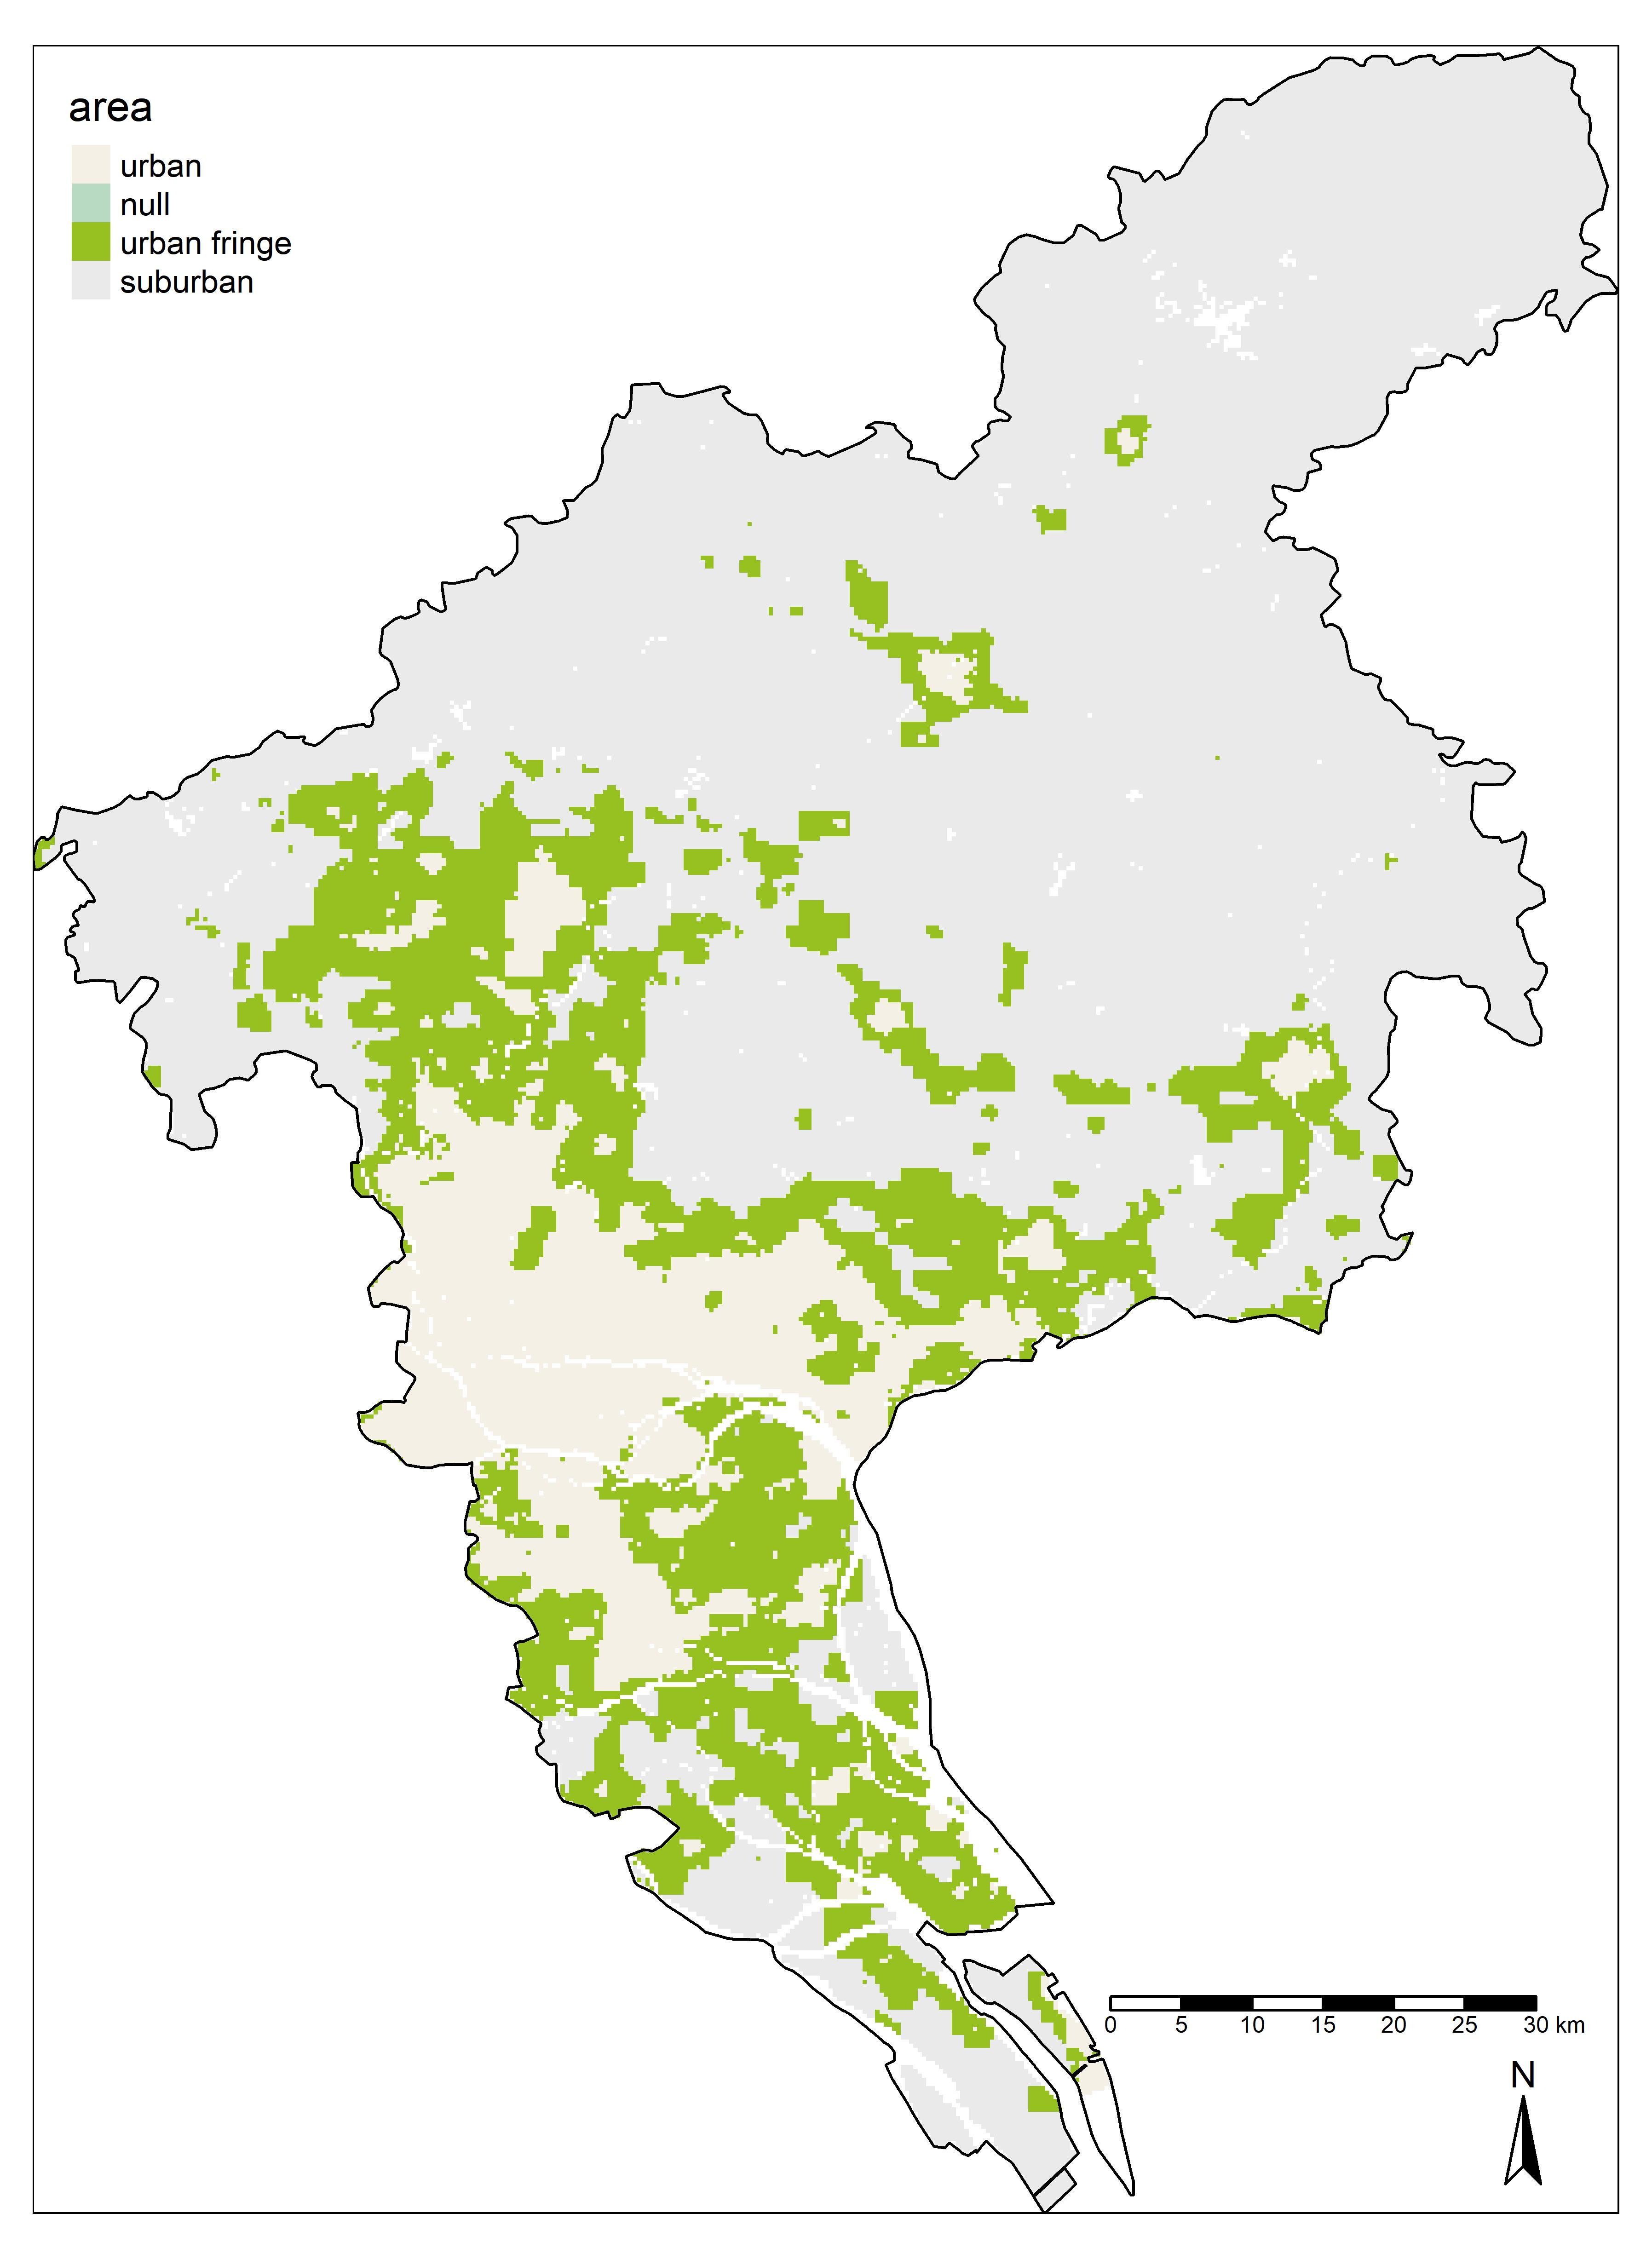
\includegraphics[width=6cm]{Figure/urbanfringegz_0821.jpg}
}
\quad
\subfigure[Shanghai]{
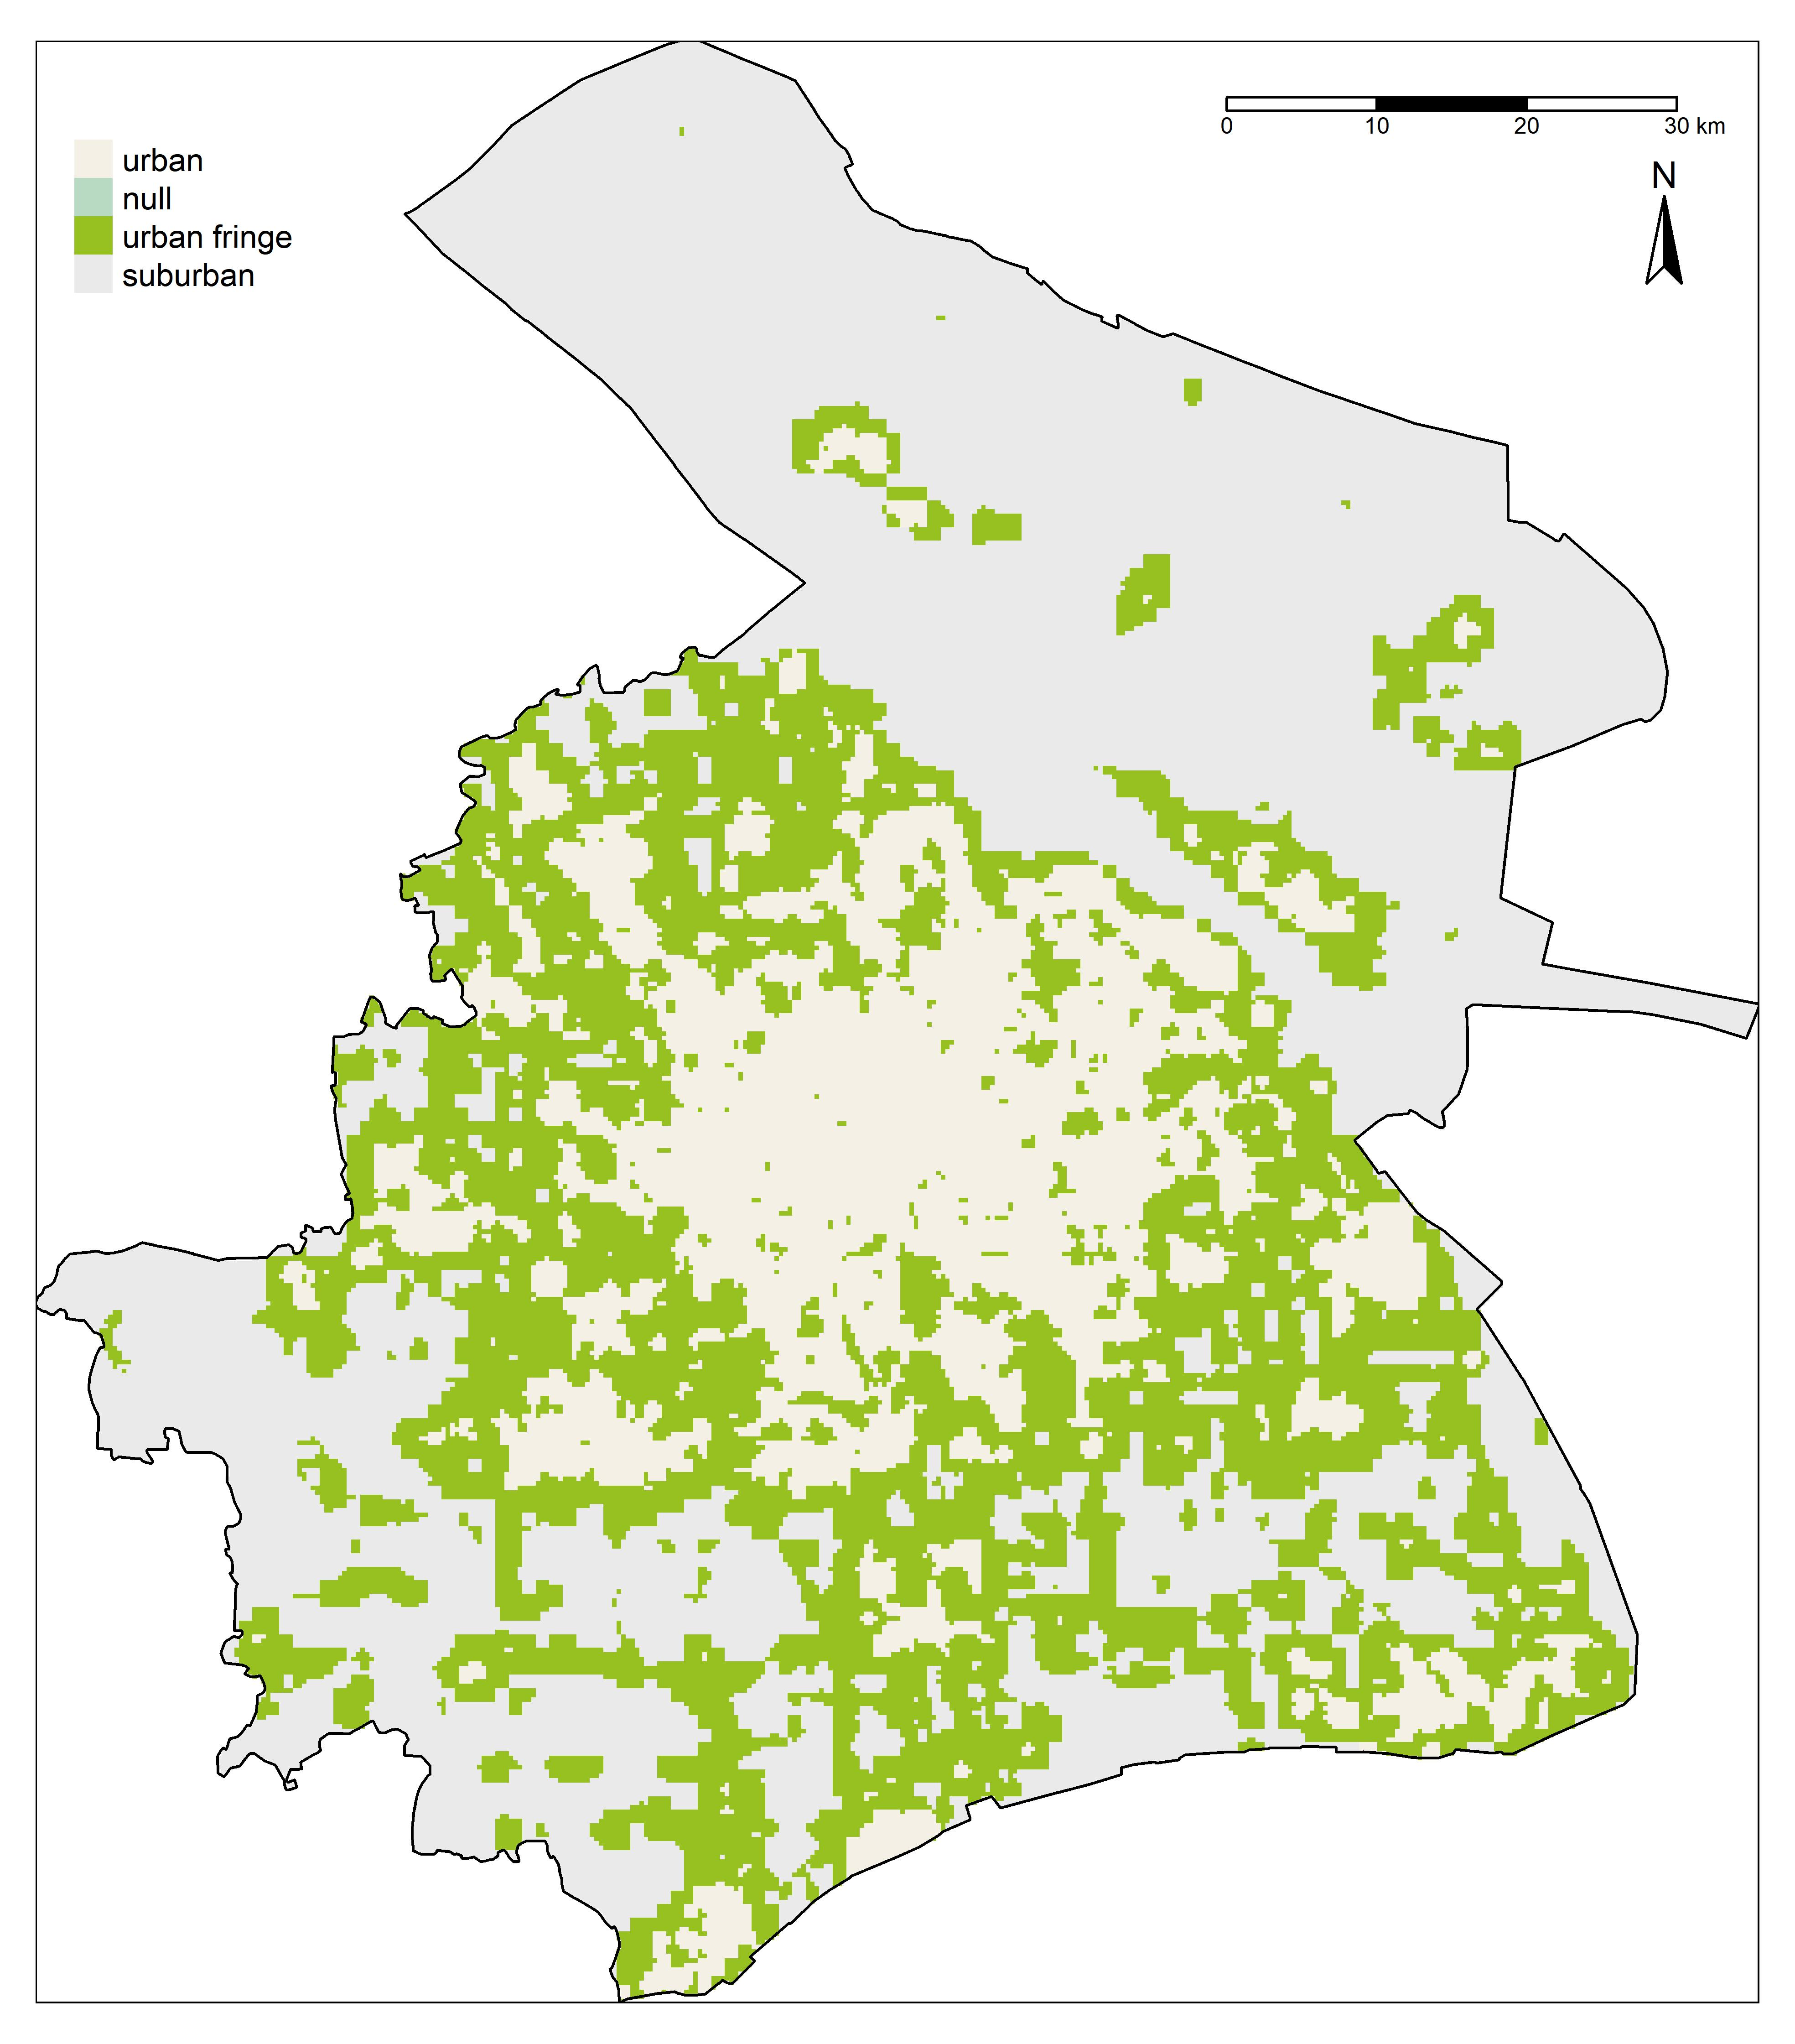
\includegraphics[width=7cm]{Figure/urbanfringe_sh0821.jpg}
}

\caption{The distribution of urban area, urban fringe area and suburban area}
\label{fringe}
\end{figure}
%%%%%%%%%%%%%%%%%%%%%%%%%%%%%%%%%%%%

\subsubsection{Shanghai}
The spatial layout of Shanghai's urban area (Figure \ref{fringe}b) was similar to that of Guangzhou, which was mainly concentrated in the central area of the city, accounting for 19.80\% of the total area. The urban fringe area, due to its distance from the urban area, was concentrated in the central and southern part of the city, accounting for 31.68\% of the total area. Suburban area was the largest area in the city and it was mainly located in the northern islands of the city. Suburban area accounted for 48.52\% of the total area.\\

When it comes to the north of the city, the two islands in the north were separated from the central area by a river because of their geographical location. Therefore, the area was not closely connected in terms of transportation and it has not been developed much in urban construction process in these years. It is clear that the urban fringe area in the northern area was the smallest part of the city and most of the land was woodland, which would be a difficult area to develop.\\

As the central area of the city, the central part of Shanghai plays an important role as the economic center, so the level of urban construction has been generally high. Most of the land types in this area were construction land. Consequently, there have been relatively more urban fringe areas.\\

As the key area for economic development in Shanghai, the southern part of the city, has identified a large number of urban fringe areas, which were distributed in a strip-like pattern in the spatial layout. This type of area would be spatially distributed in the form of strips, which could be interspersed with urban area and suburban to form a network spatial shape.\\


\subsection{Descriptive statistics}

%%%%%%%%%%%%%%%%%%%%%%%%%%%%%%%%%%%%%%%%%%%%%%%%%%%%%%%

\begin{table}[H]
\caption{The general statistics of indicators from 2 systems in Guangzhou and Shanghai}
\label{statistics}
\centering
\begin{tabular}{>{\hspace{0pt}}m{0.25\linewidth}>{\hspace{0pt}}m{0.107\linewidth}>{\hspace{0pt}}m{0.073\linewidth}>{\hspace{0pt}}m{0.109\linewidth}>{\hspace{0pt}}m{0.09\linewidth}>{\hspace{0pt}}m{0.073\linewidth}>{\hspace{0pt}}m{0.127\linewidth}} 
\hline
\multicolumn{1}{>{\hspace{0pt}}m{0.25\linewidth}|}{}                  & \multicolumn{3}{>{\centering\hspace{0pt}}m{0.289\linewidth}|}{\textbf{Guangzhou}}                & \multicolumn{3}{>{\centering\arraybackslash\hspace{0pt}}m{0.29\linewidth}}{\textbf{Shanghai}}  \\ 
\cline{2-7}
\multicolumn{1}{>{\hspace{0pt}}m{0.25\linewidth}|}{\textbf{Indcator}} & \textbf{Max} & \textbf{Min} & \multicolumn{1}{>{\hspace{0pt}}m{0.109\linewidth}|}{\textbf{Mean}} & \textbf{Max} & \textbf{Min} & \textbf{Mean}                                                    \\ 
\hline
\textbf{Socio-economic index}                                          & 0.97         & 0            & 0.21                                                               & 0.92         & 0            & 0.3                                                              \\
\textbf{AL}                                                            & 1            & 0            & 0.18                                                               & 1            & 0            & 0.30~                                                            \\
\textbf{CL}                                                            & 75.87        & 0            & 21.78                                                              & 76.23        & 0            & 13.82                                                            \\
\textbf{NT}                                                            & 331.15       & 0            & 8.19                                                               & 371.3        & 0            & 14.09                                                            \\
\textbf{Environmental index}                                           & 0.97         & 0.24         & 0.64                                                               & 0.92         & 0.12         & 0.58                                                             \\
\textbf{NDVI}                                                          & 0.85         & 0            & 0.55                                                               & 0.85         & 0            & 0.43                                                             \\
\textbf{NPP}                                                           & 14141        & 0            & 6484.2                                                             & 9862         & 0            & 3343.16                                                          \\
\textbf{PM2.5}                                                         & 34.6         & 23.5         & 28.22                                                              & 45.9         & 26.4         & 32.99                                                            \\
\hline
\end{tabular}
\end{table}

%%%%%%%%%%%%%%%%%%%%%%%%%%%%%%%%%%%%%%%%%%%%%%%%%%%%%%%

\subsubsection{Socio-economic index}
Figure \ref{ugz} and \ref{ush} showed the performance of each indicator from urban development system in 2019 from Guangzhou and Shanghai. Table \ref{statistics} showed the general statistics of each indicator including average value in these two cities. Socio-economic index in the large area of high-values from Guangzhou was concentrated in the central part of the city. It was worth noting that the continuous and high-value areas were mostly located on both sides of the rivers in the central part. Compared to this, the southern areas were fragmented but the high-value areas were still evenly distributed over the spatial area. As we could see within the northern area, there were certain variations, with only a few high-value spaces in the northeast part due to the influence of woodland and other ecological green spaces. While in the northwest part of the area, there were fragmented but concentrated areas near the central river. Through the analysis of the socio-economic index, we could further consider a method to connect this area through land consolidation and other measures, so that the urban space could be used more efficiently.\\

When it comes to Shanghai, the socio-economic index with a large range of high-value areas was concentrated in the central part of the city near the south of the river. The urban construction areas in the central area would show a concentrated and centralized pattern. Besides, the northern part of the city had almost no high-value areas due to the poor river connectivity with the central part of the city. What is worth mentioning is that the areas with high index were all close to the river and the southern part of the central part of the city.\\

When comparing the difference between Guangzhou and Shanghai, The highest values in Guangzhou are higher than those in Shanghai. Guangzhou had relatively few high-value areas In terms of spatial distribution, and they were also very concentrated in the central area. The high-value areas in Shanghai were distributed evenly in most of the city-wide areas. This also indicated that Guangzhou's development in some areas was relatively more prominent than in other areas, while SH showed more nodal and core development characteristics within the areas due to its uniform distribution. In addition, the average value of Shanghai socio-economic index was larger than that of Guangzhou, which means that the economic level of Shanghai was much higher than that of Guangzhou.\\

%%%%%%%%%%%%%%%%%%%%%%%%%%%%%%%%%%%%
\begin{figure}[H]
\centering
\subfigure[Socio-economic index]{
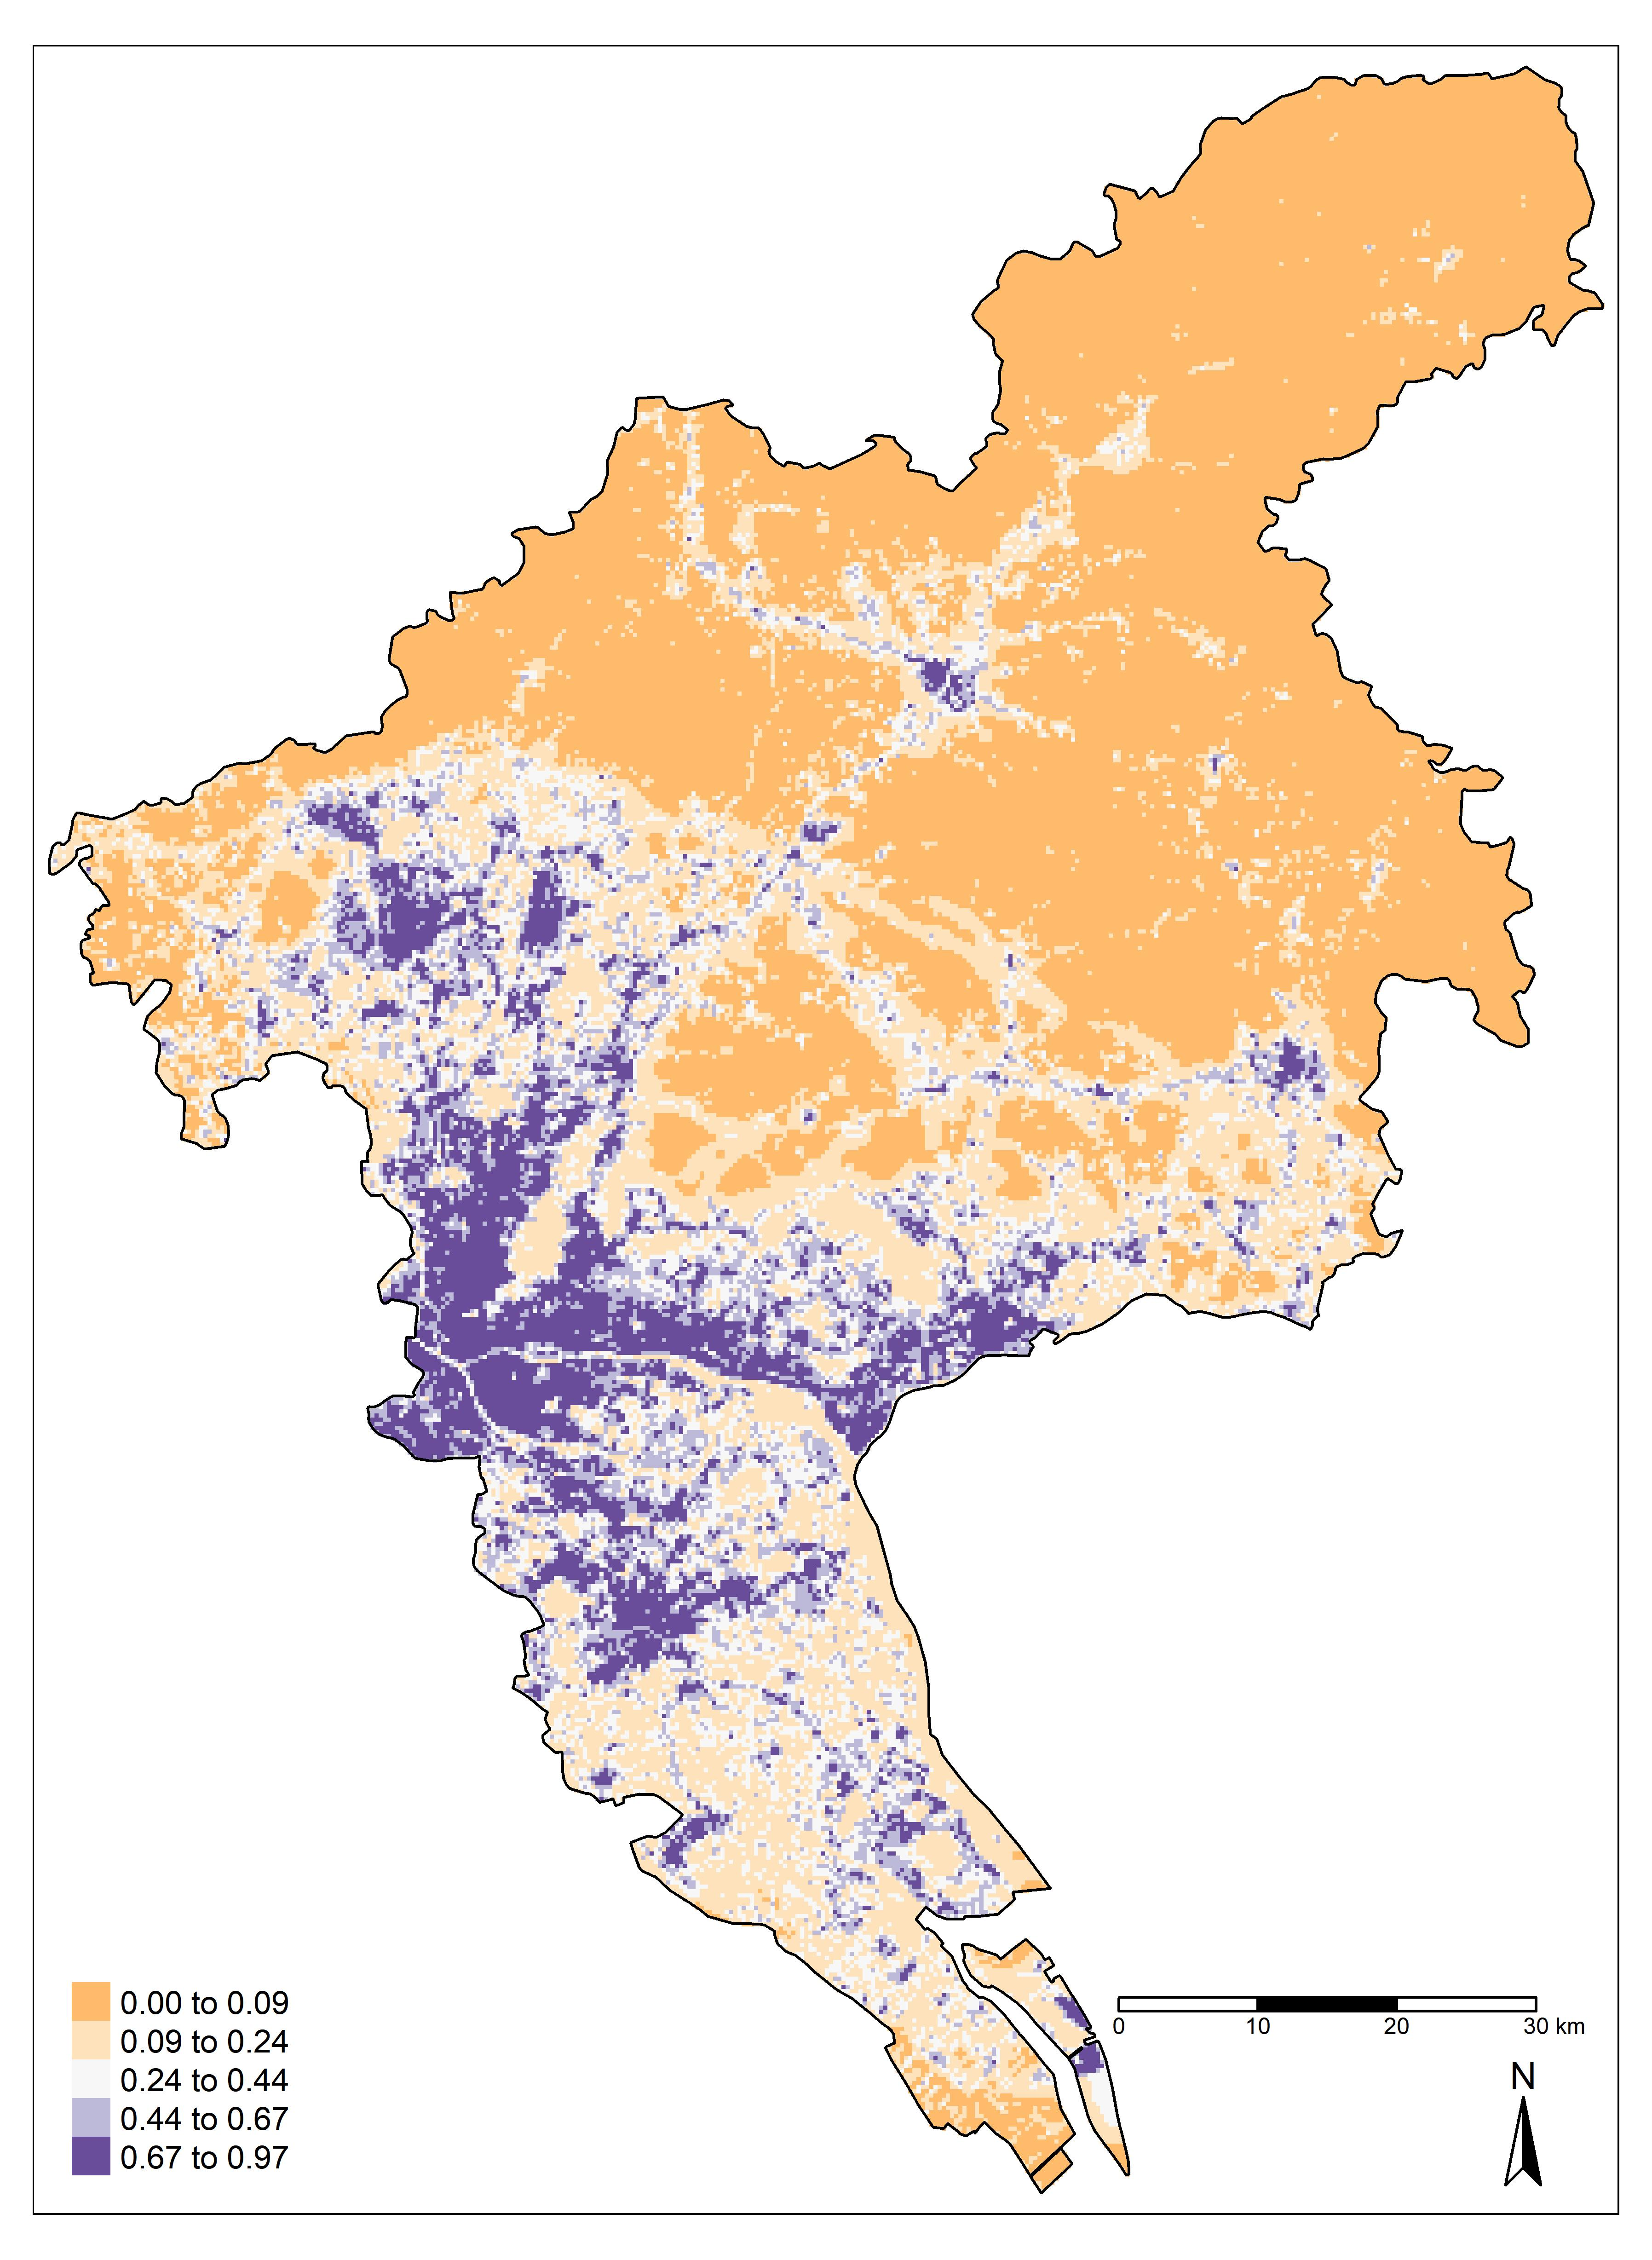
\includegraphics[width=6cm]{Figure/ugz.jpg}
}
\quad
\subfigure[AL]{
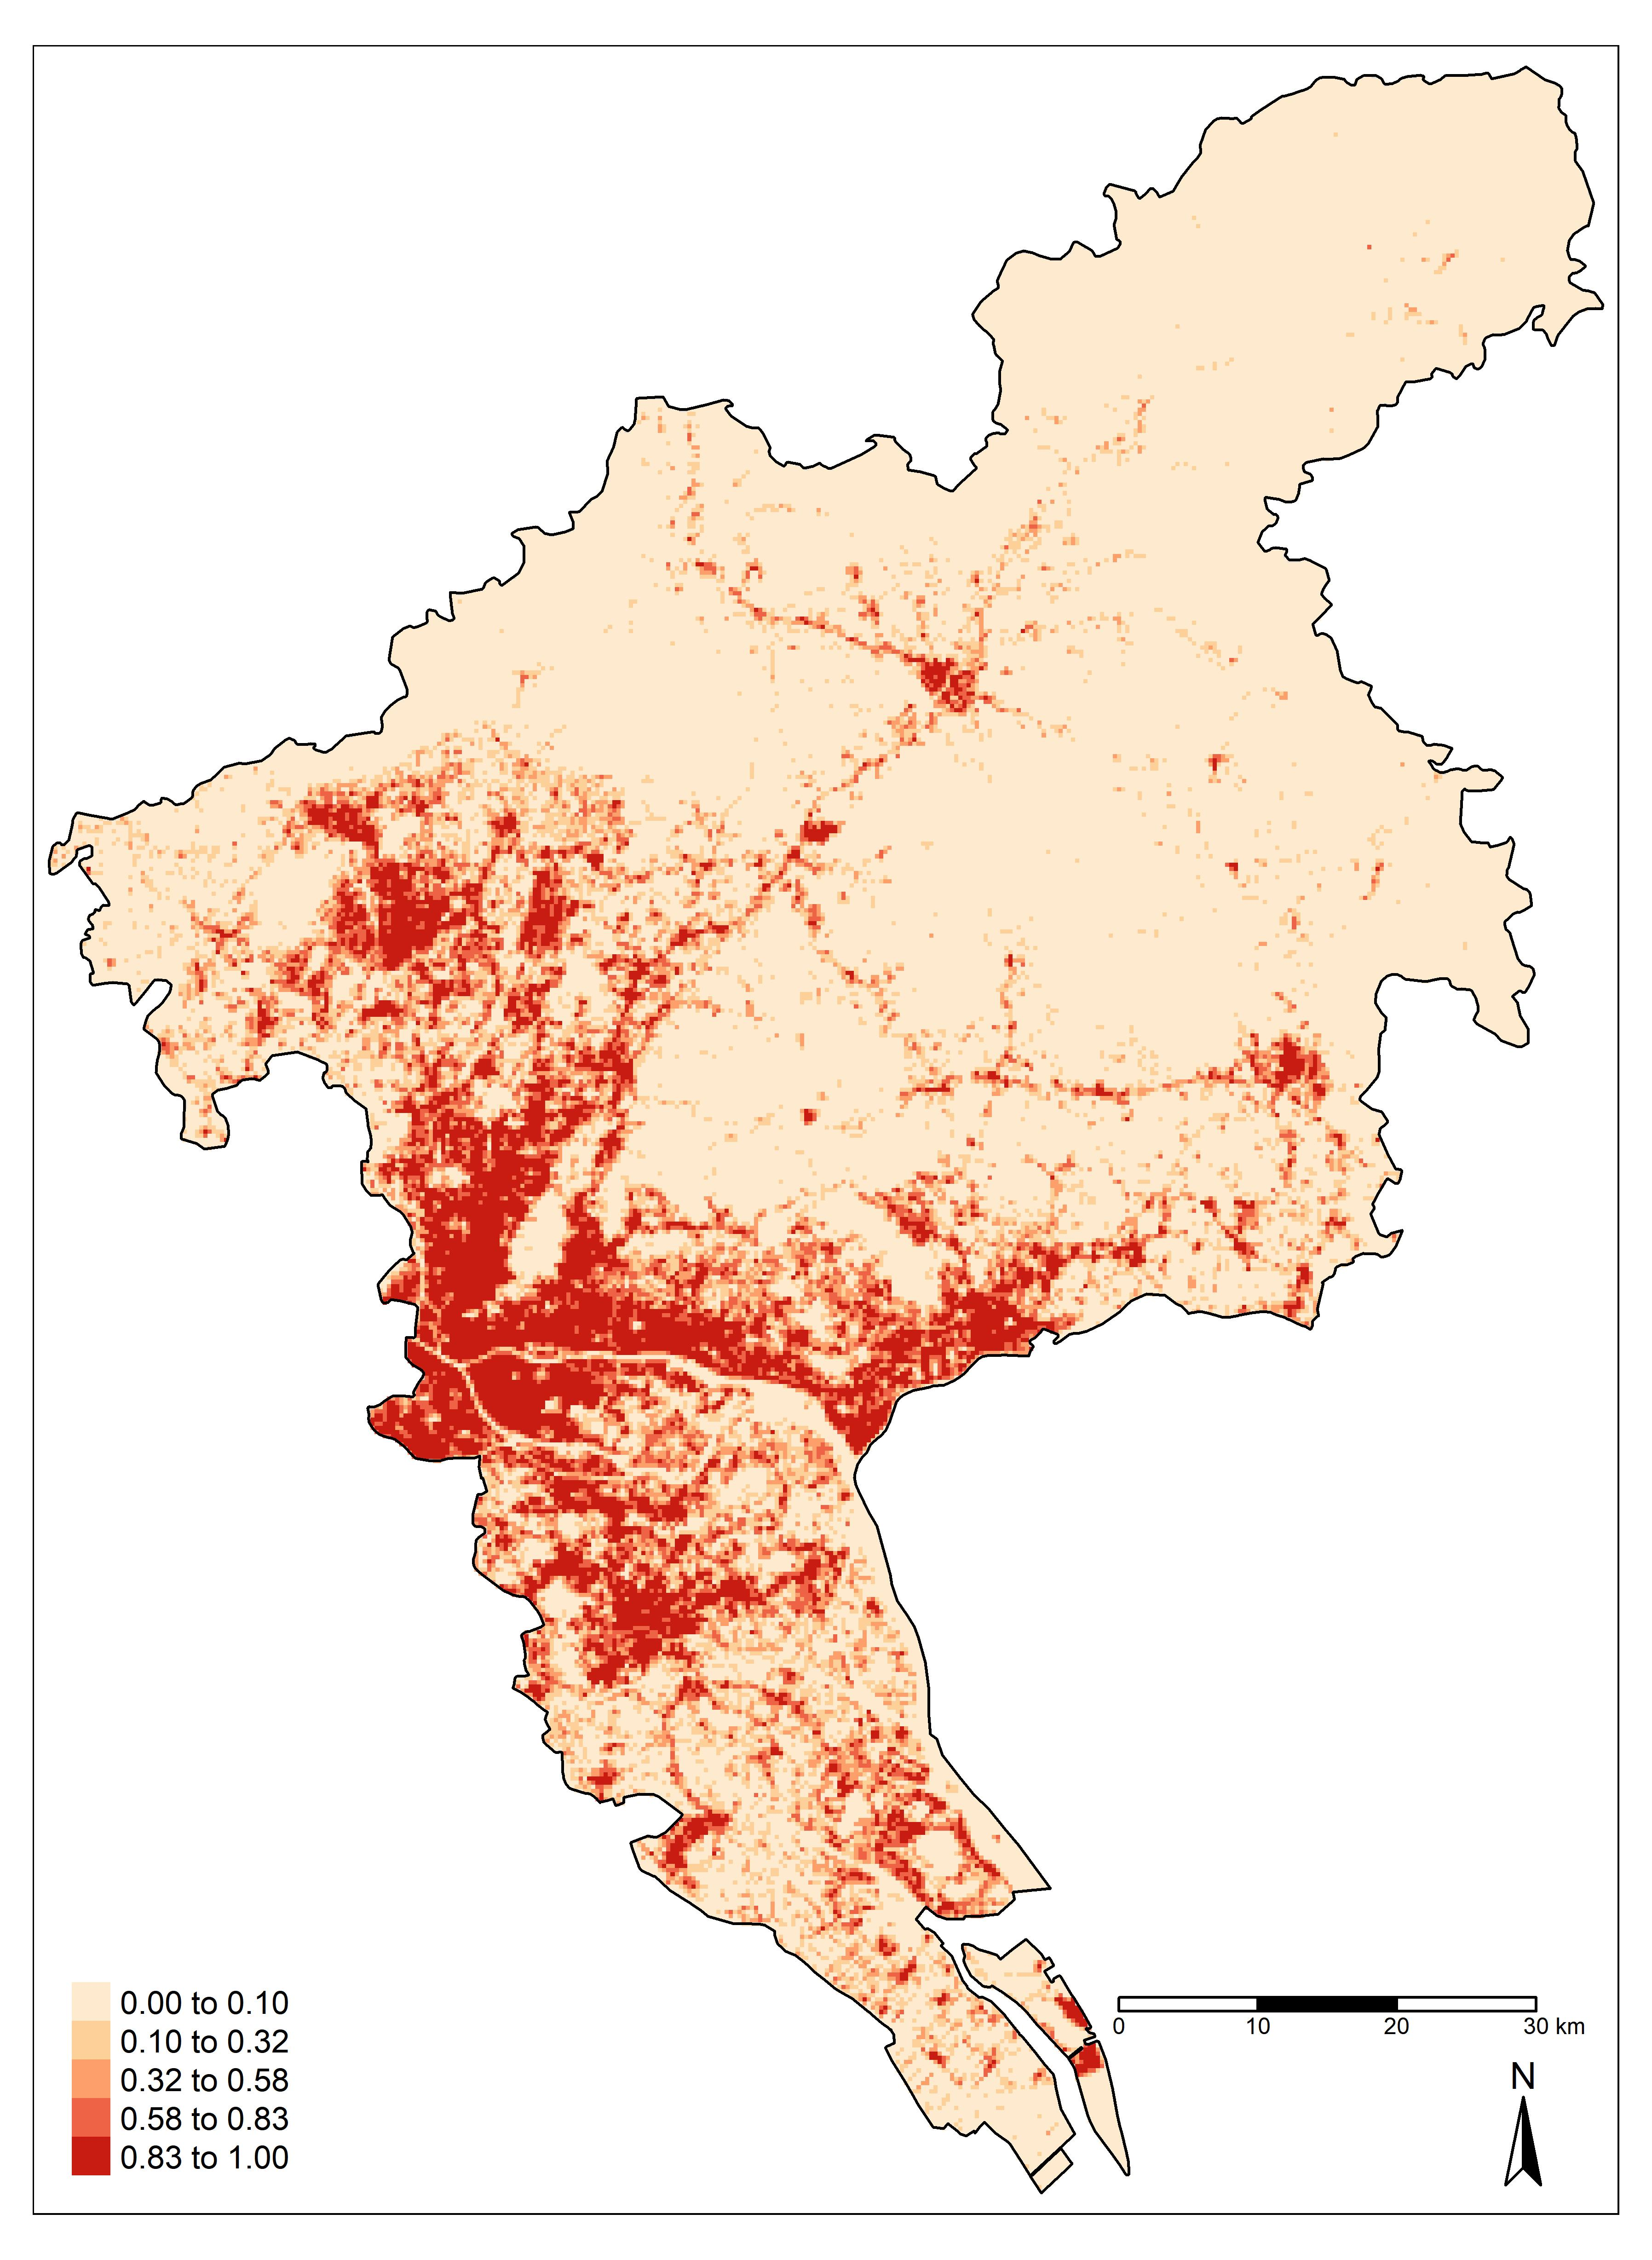
\includegraphics[width=6cm]{Figure/area_gz.jpg}
}
\quad
\subfigure[CL]{
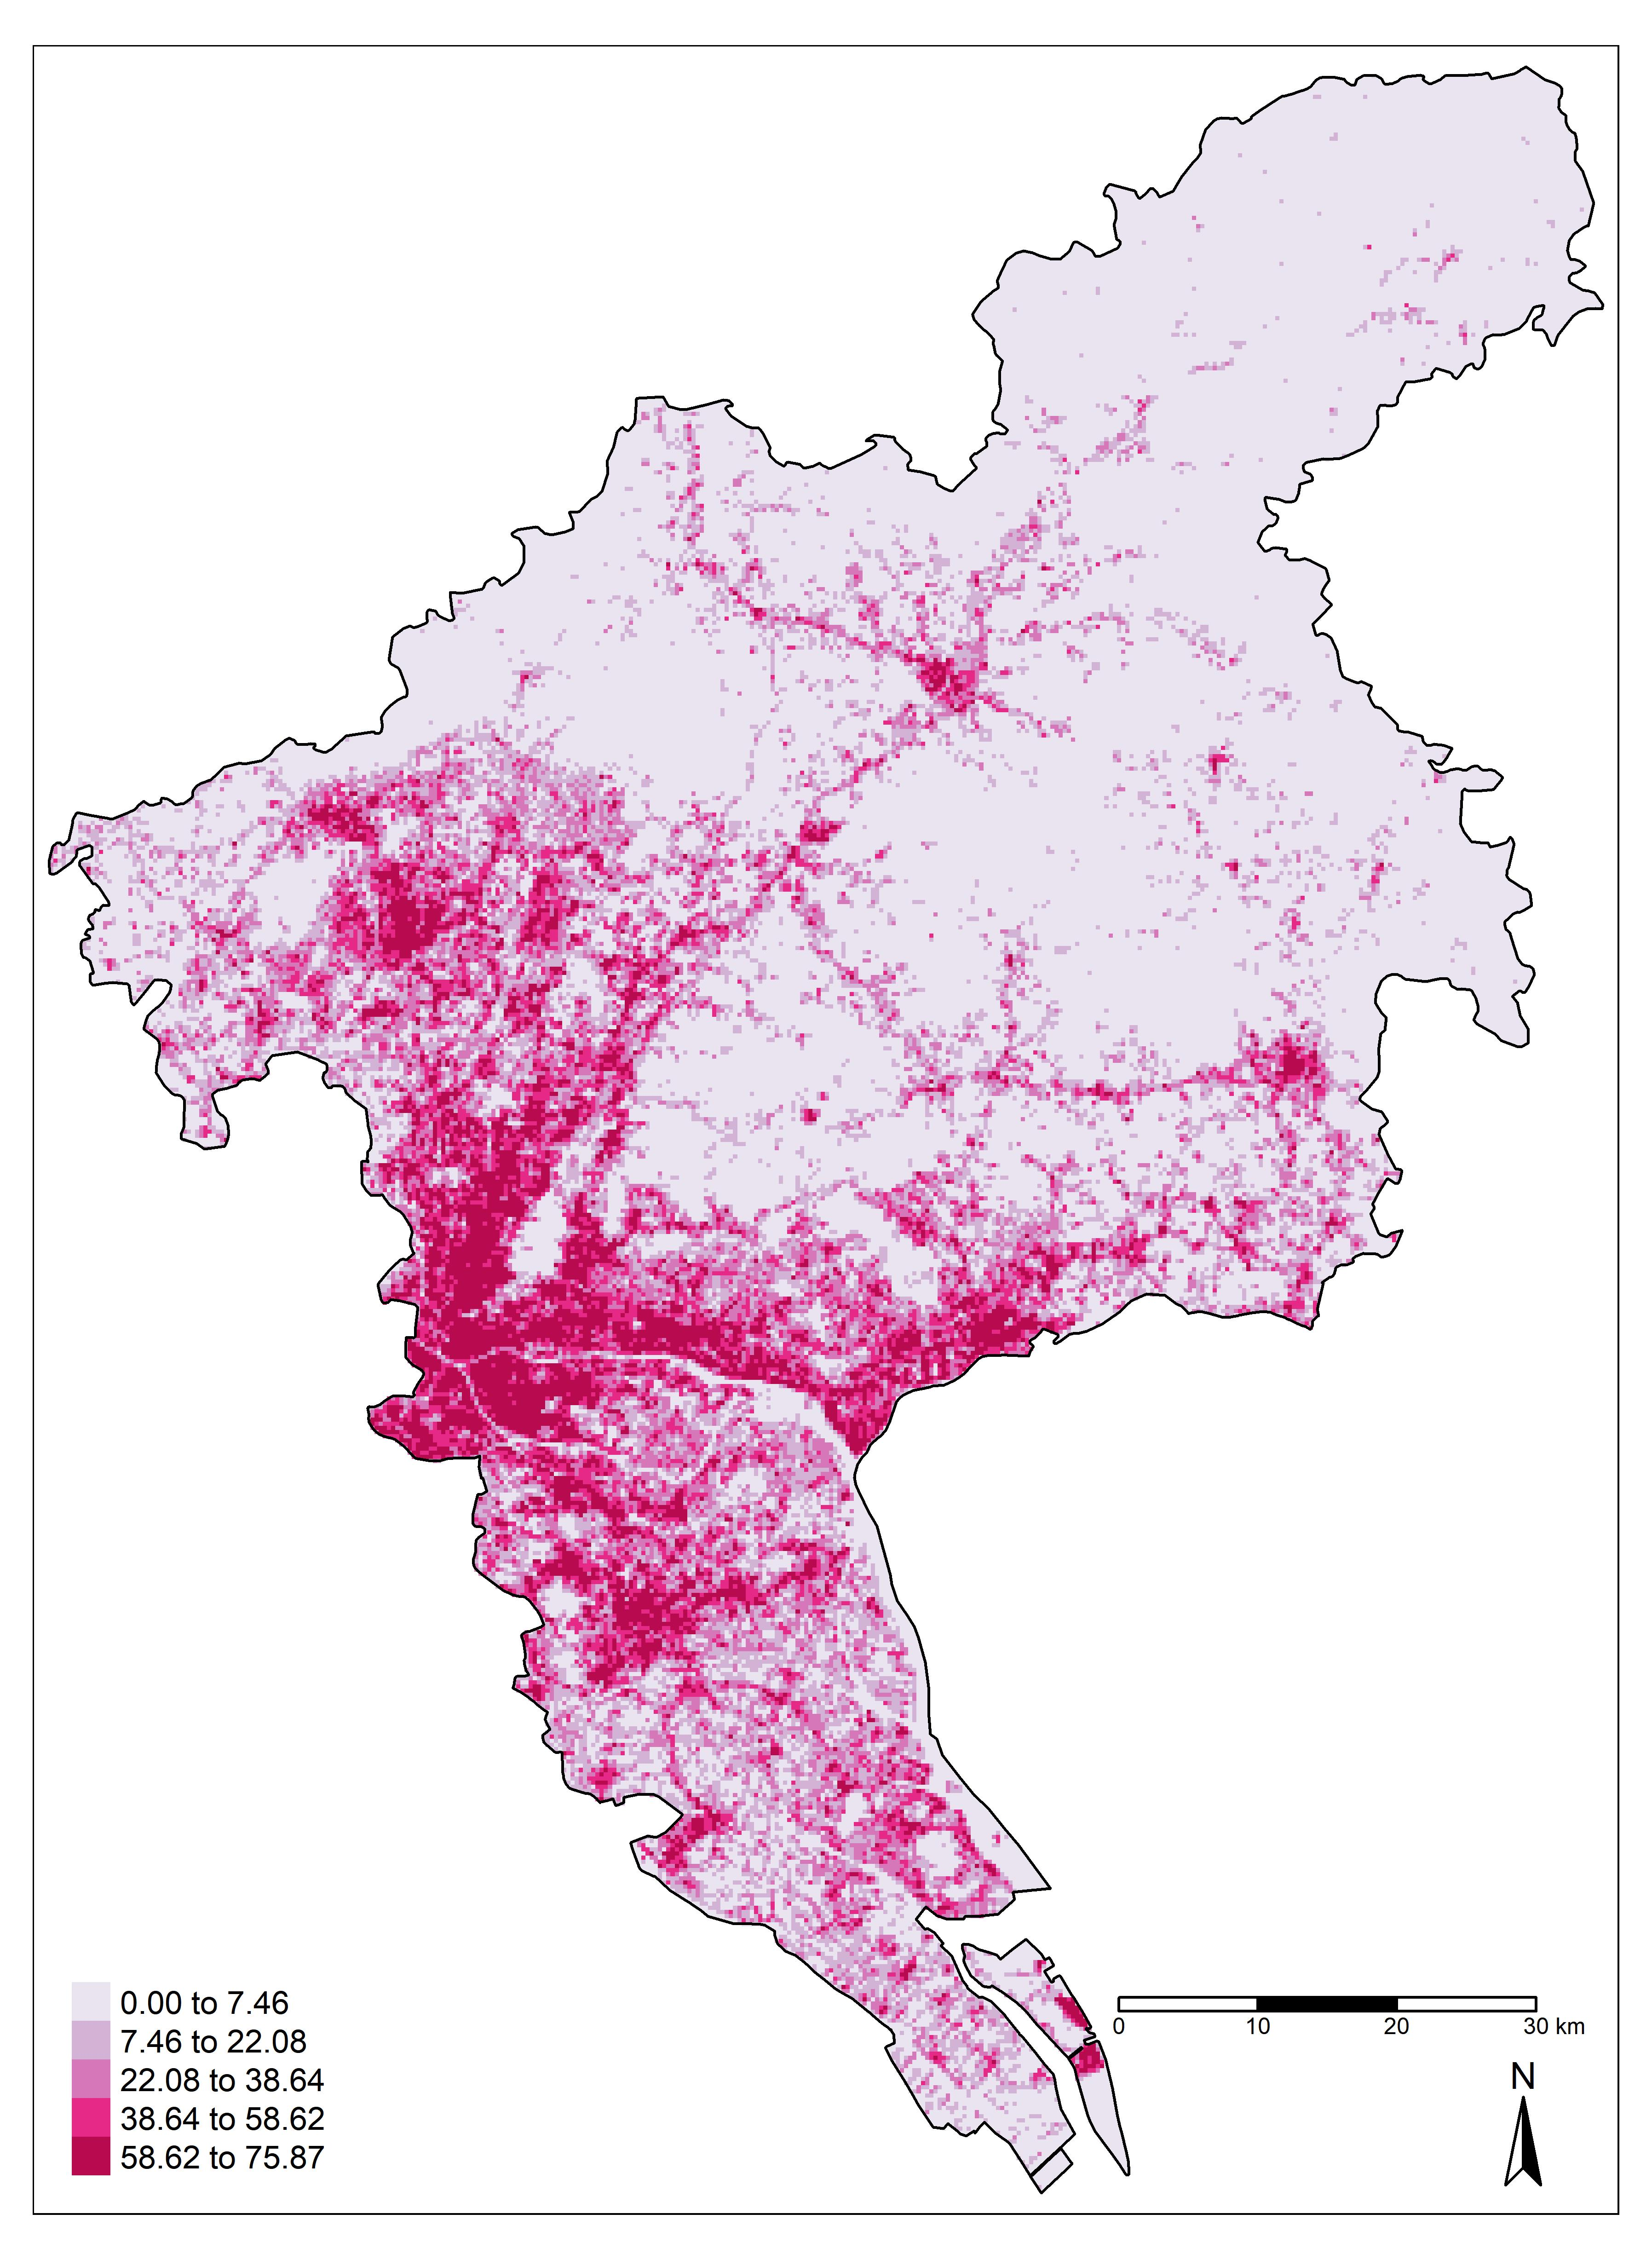
\includegraphics[width=6cm]{Figure/length_gz.jpg}
}
\quad
\subfigure[NT]{
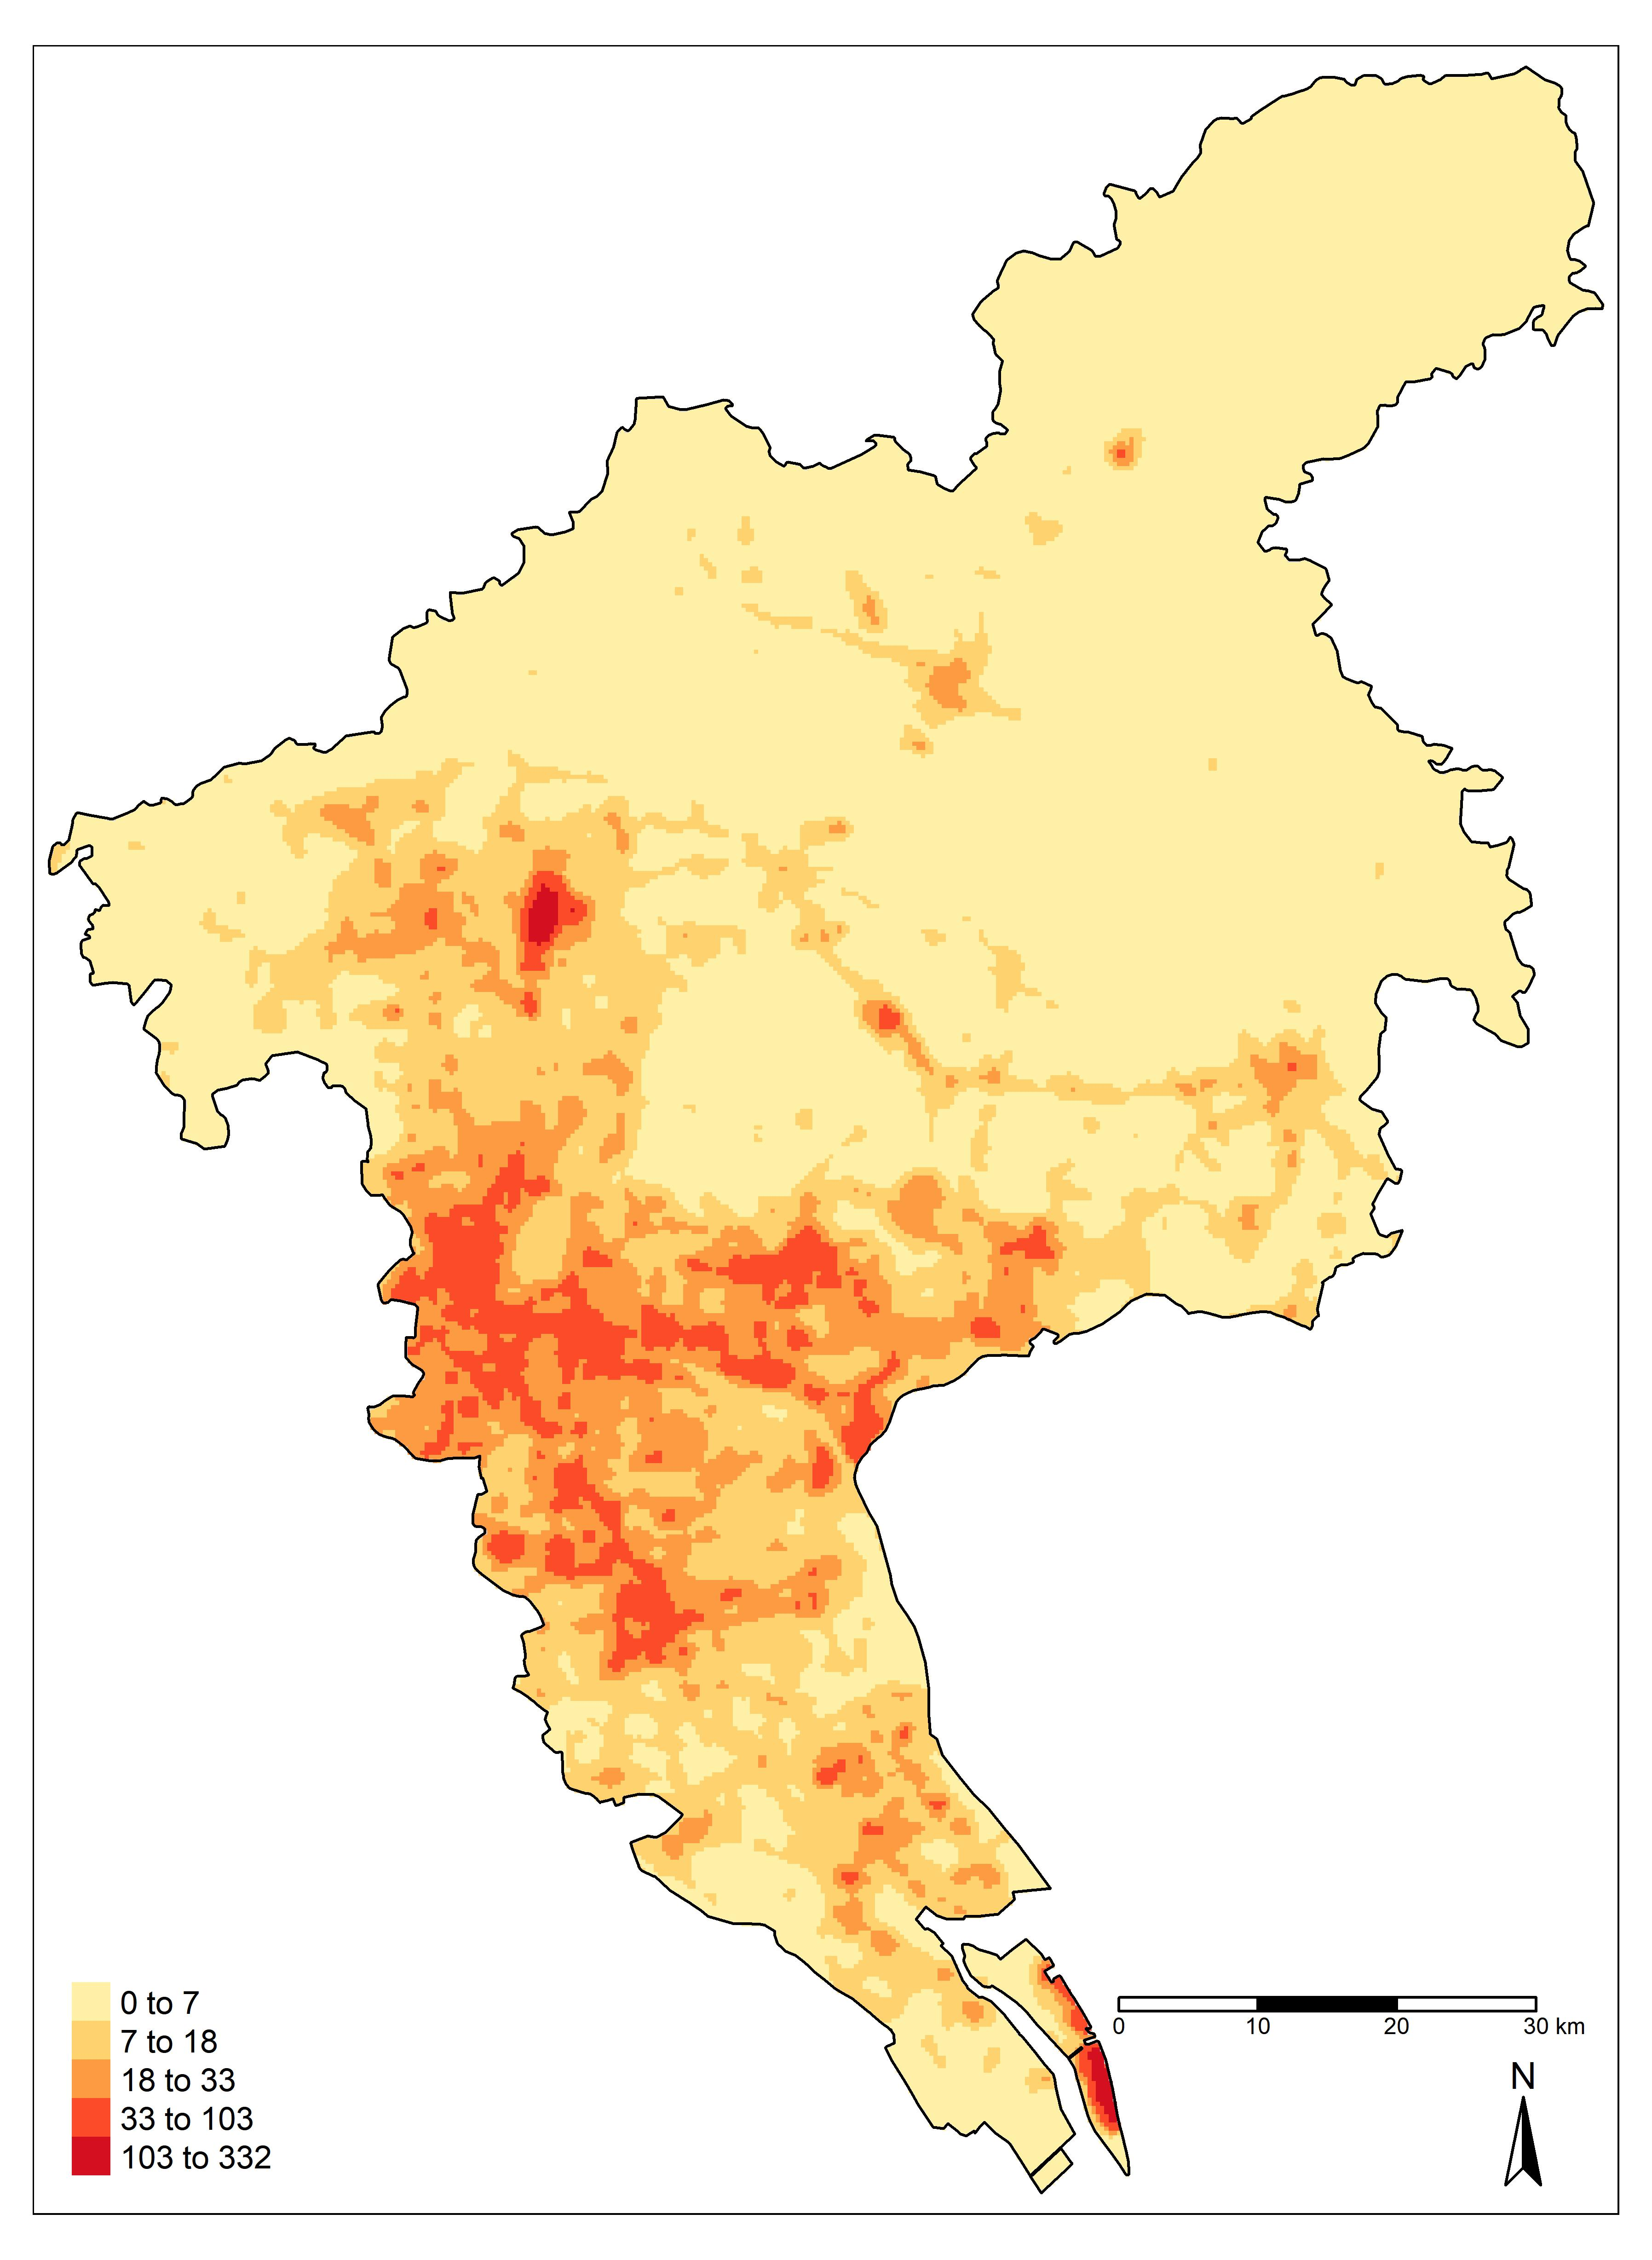
\includegraphics[width=6cm]{Figure/nt_gz.jpg}
}
\caption{Indicators of urban development system in Guangzhou}
\label{ugz}
\end{figure}
%%%%%%%%%%%%%%%%%%%%%%%%%%%%%%%%%%%%

%%%%%%%%%%%%%%%%%%%%%%%%%%%%%%%%%%%%
\begin{figure}[H]
\centering
\subfigure[Socio-economic index]{
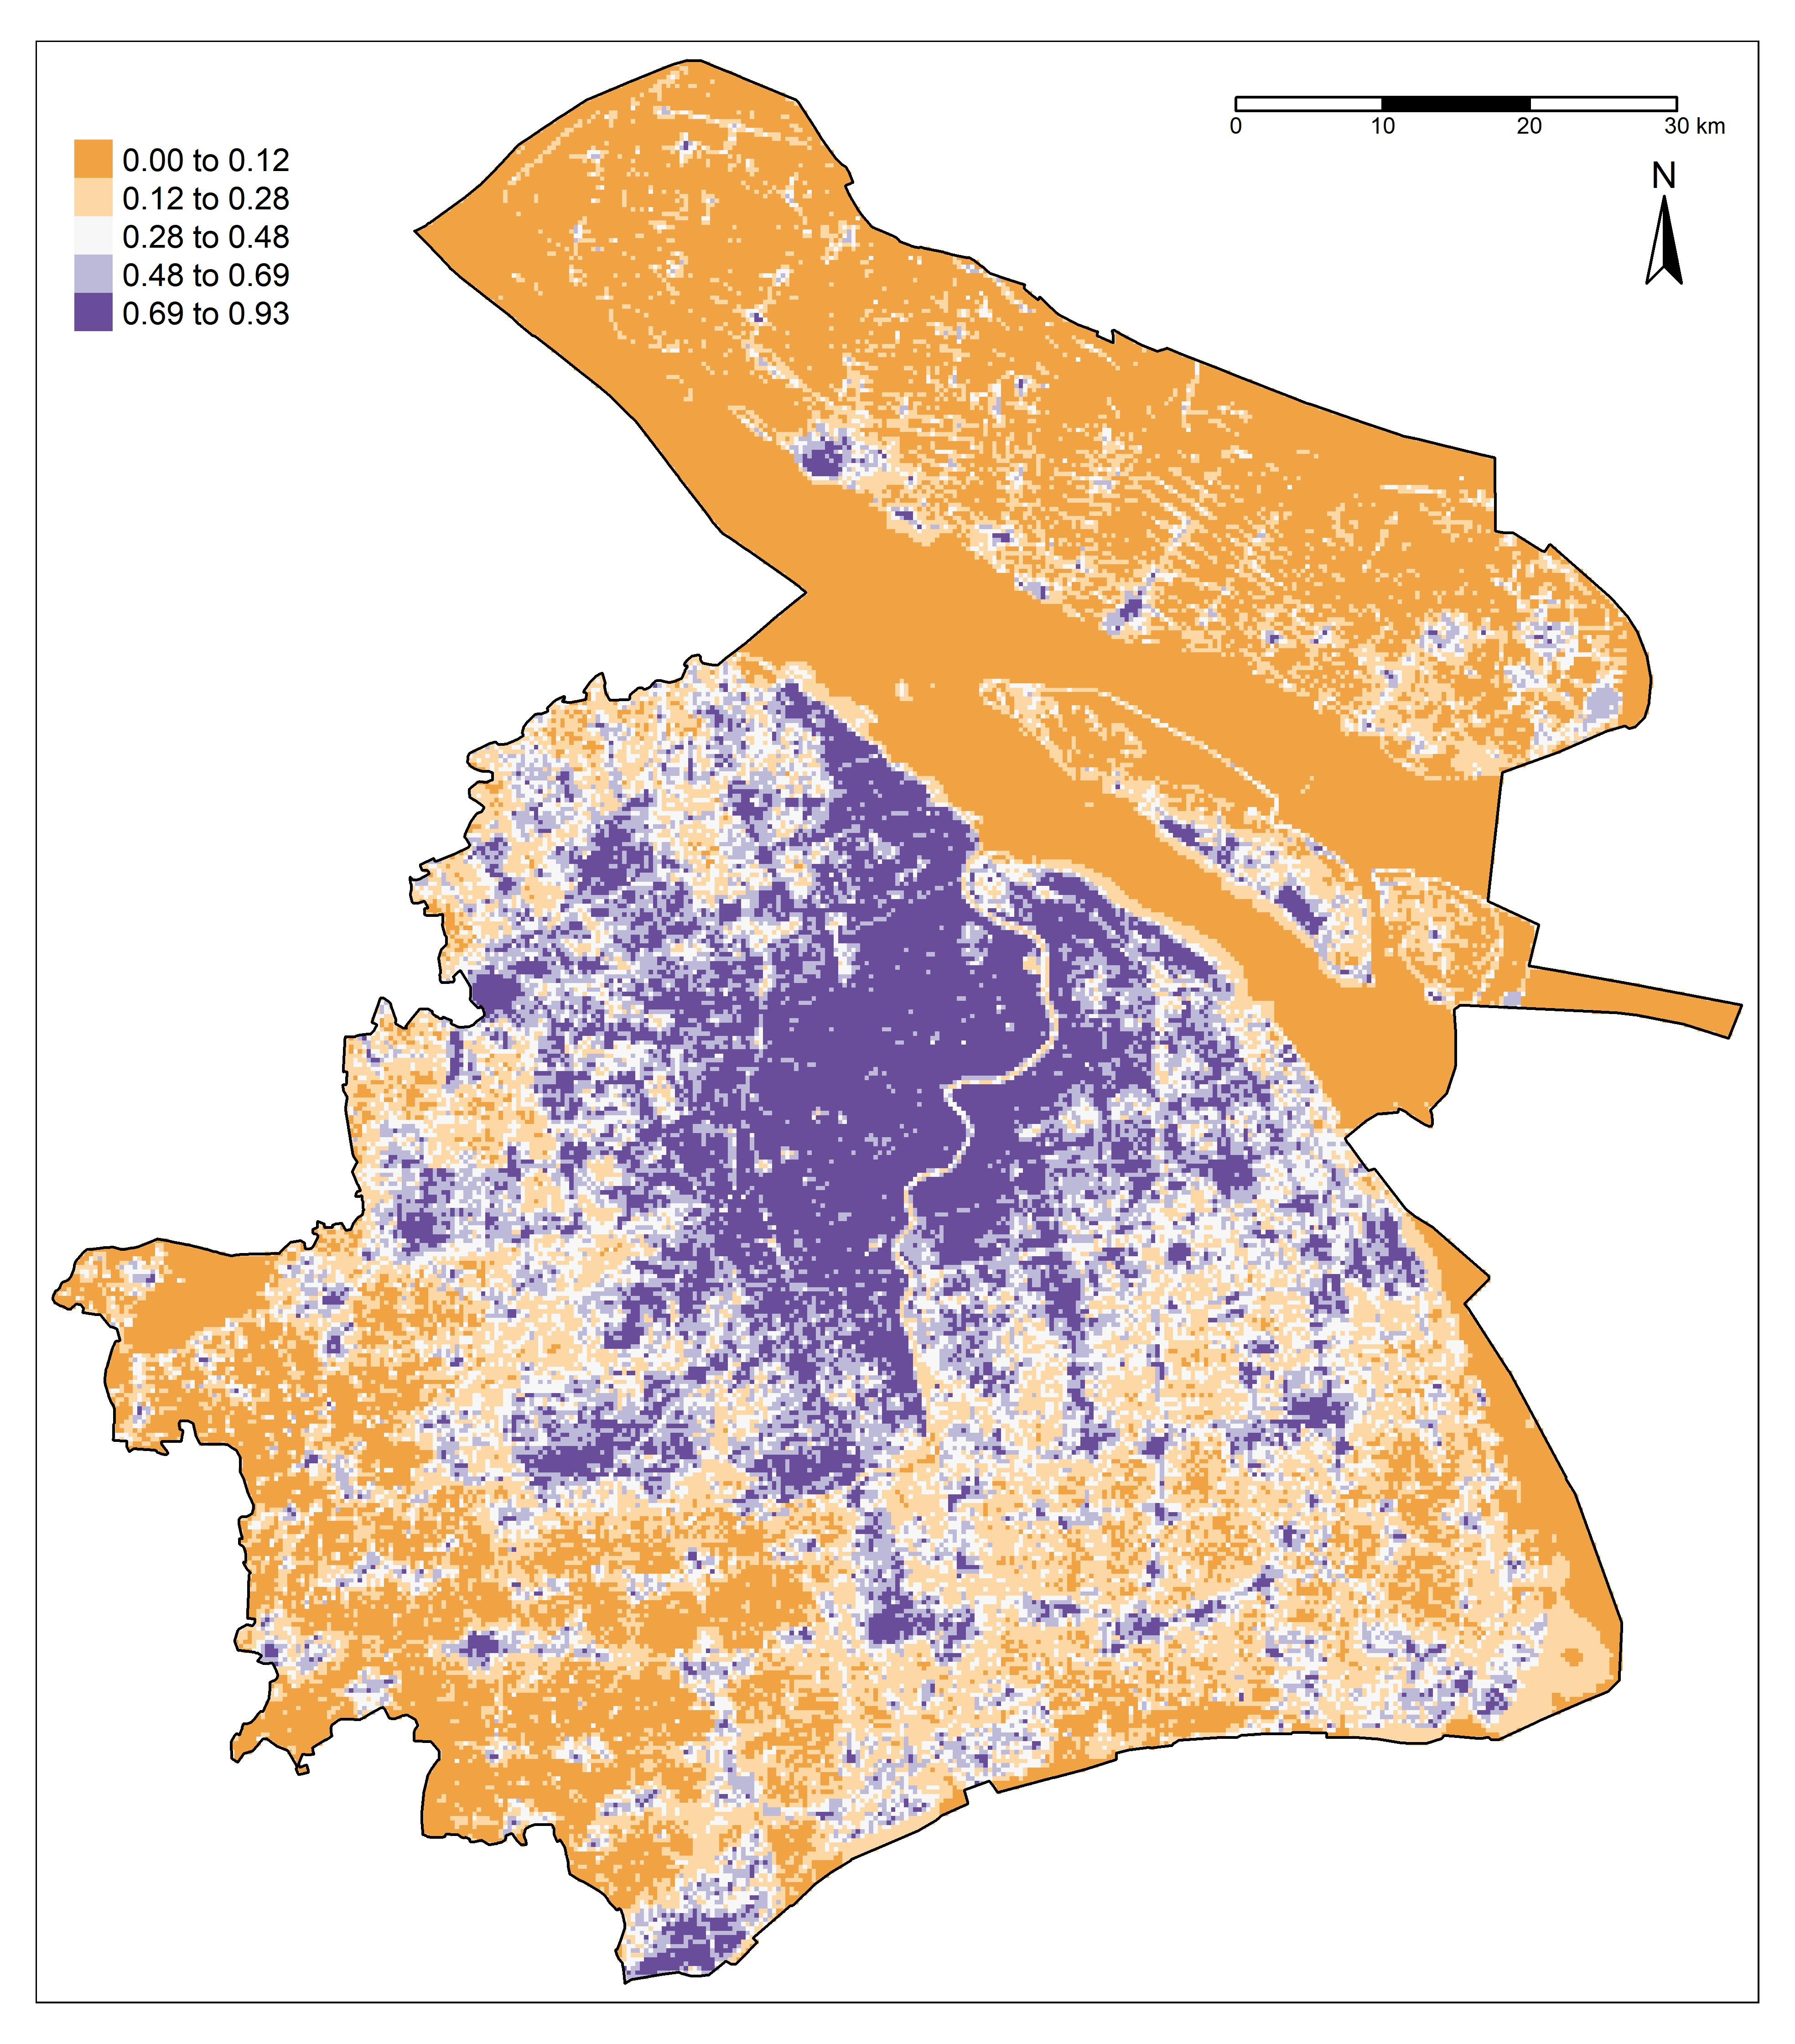
\includegraphics[width=6cm]{Figure/ush.jpg}
}
\quad
\subfigure[AL]{
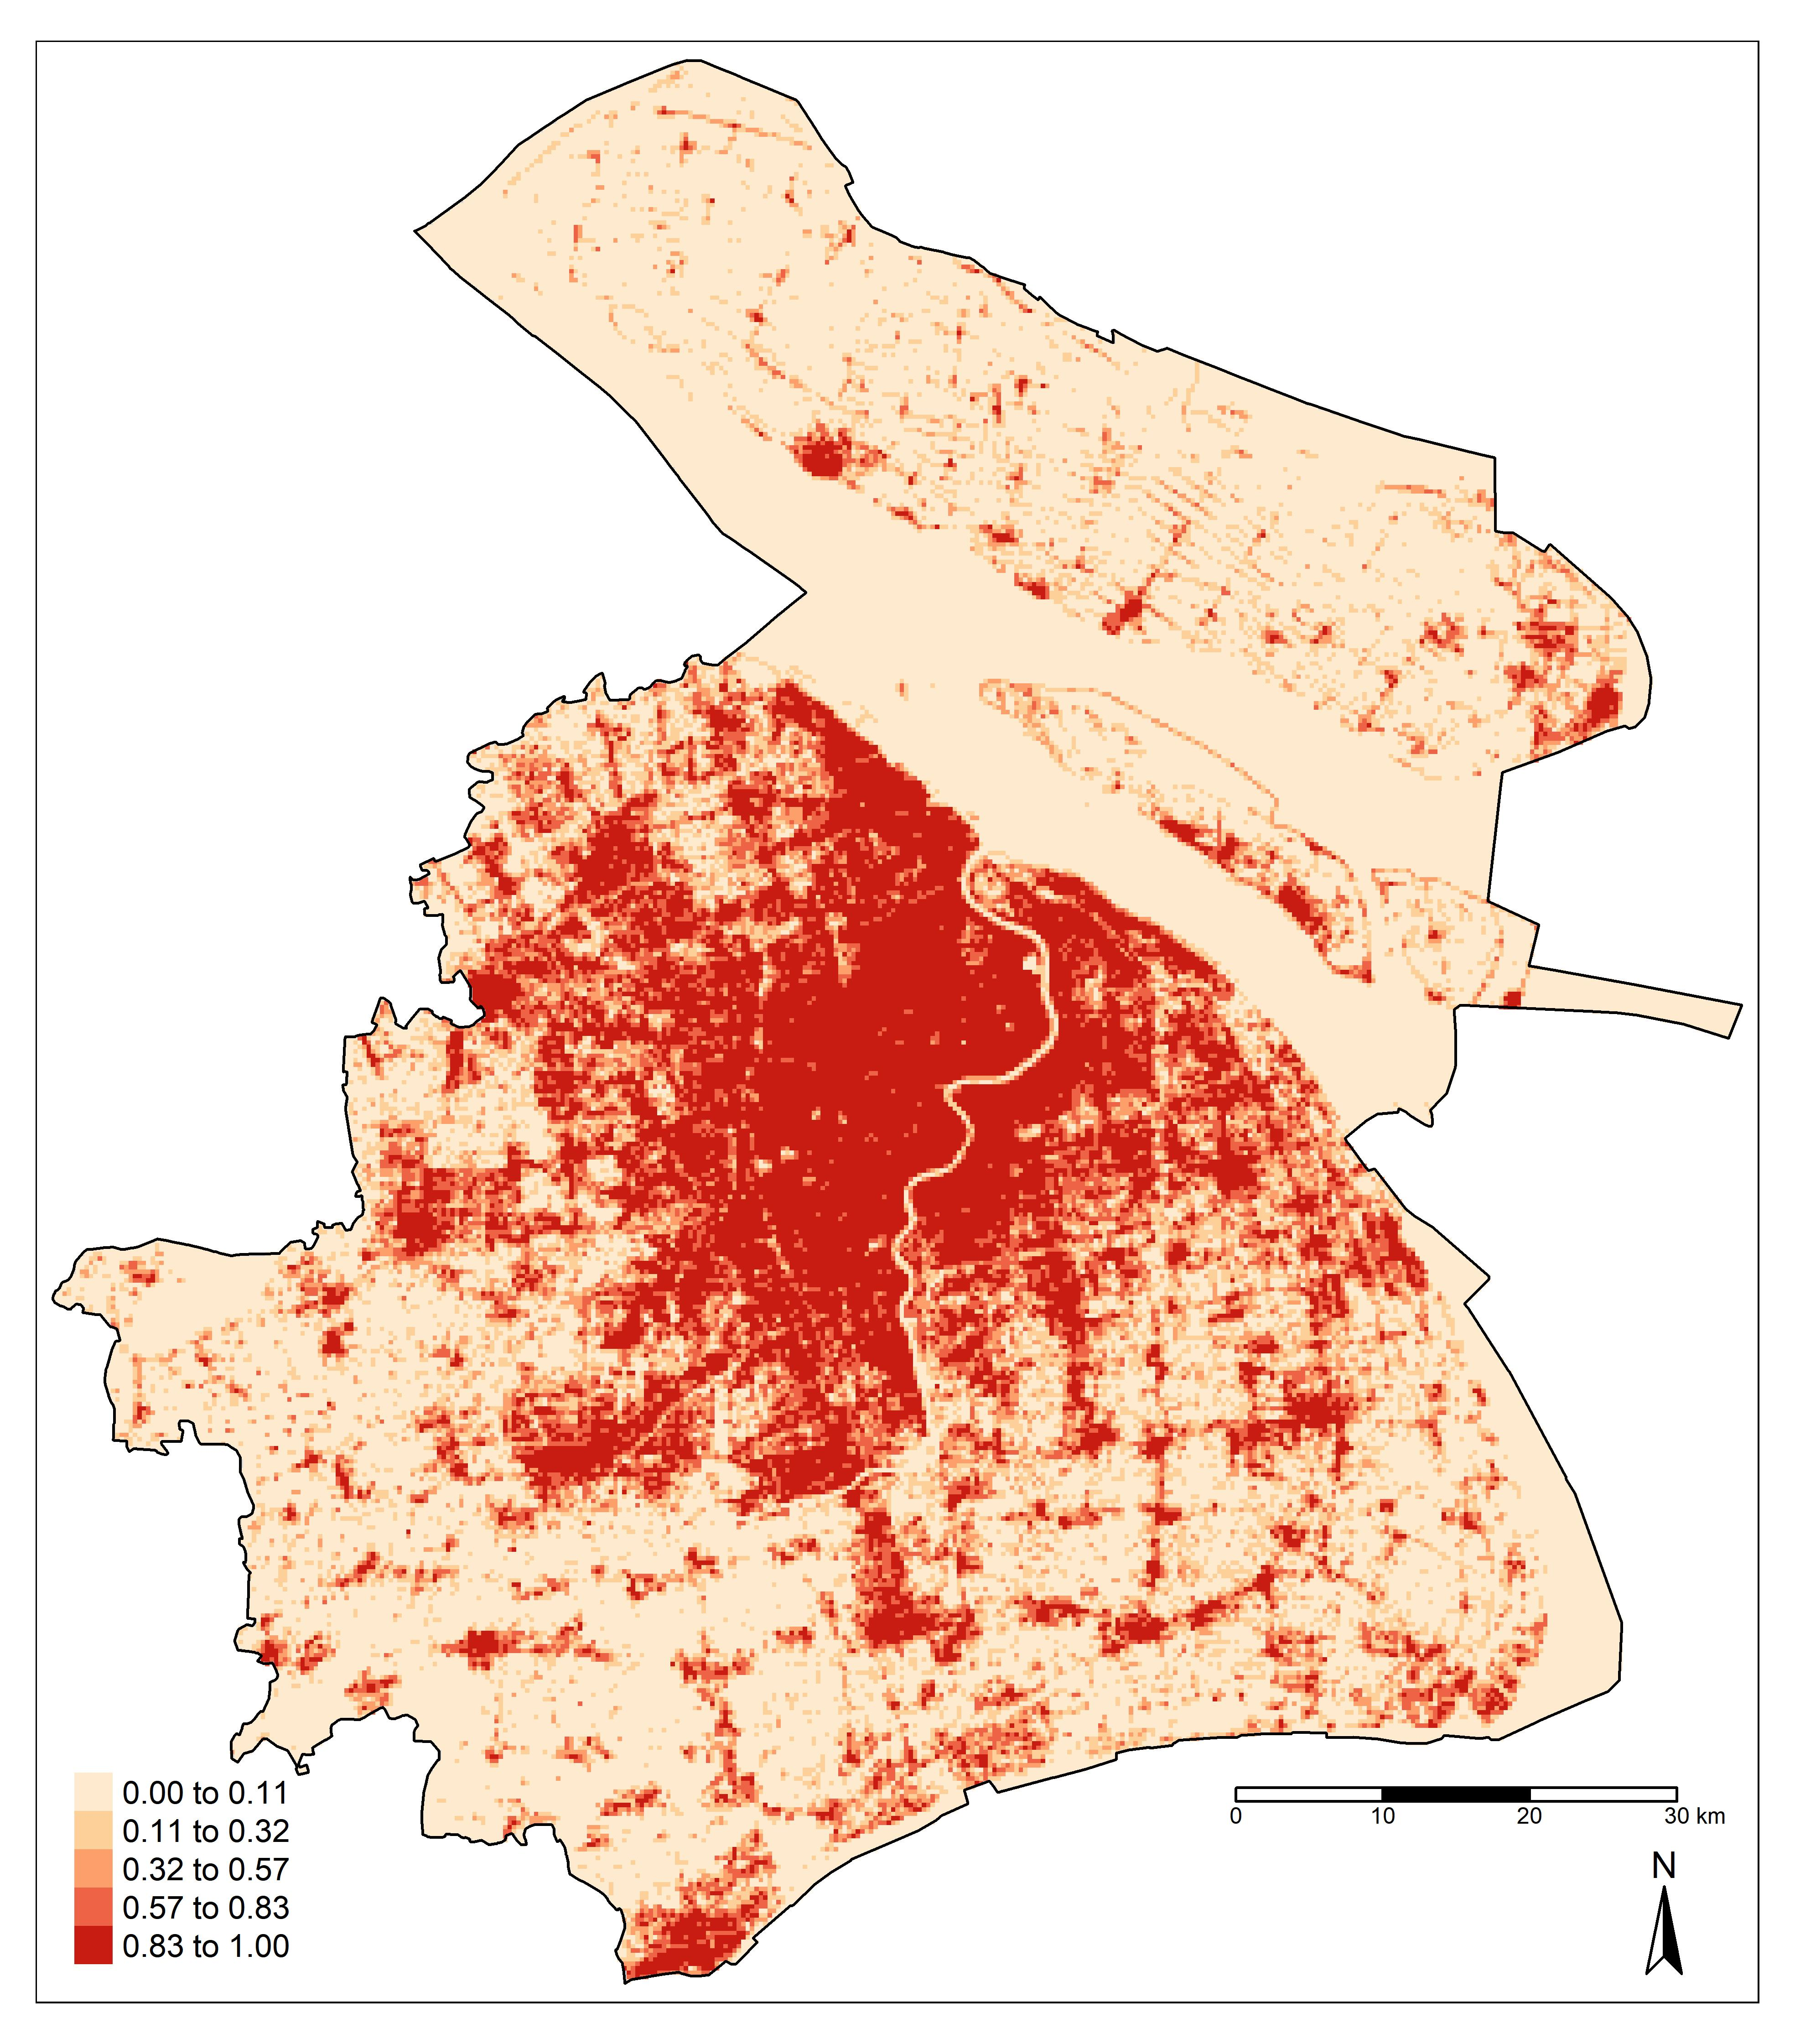
\includegraphics[width=6cm]{Figure/area_sh.jpg}
}
\quad
\subfigure[CL]{
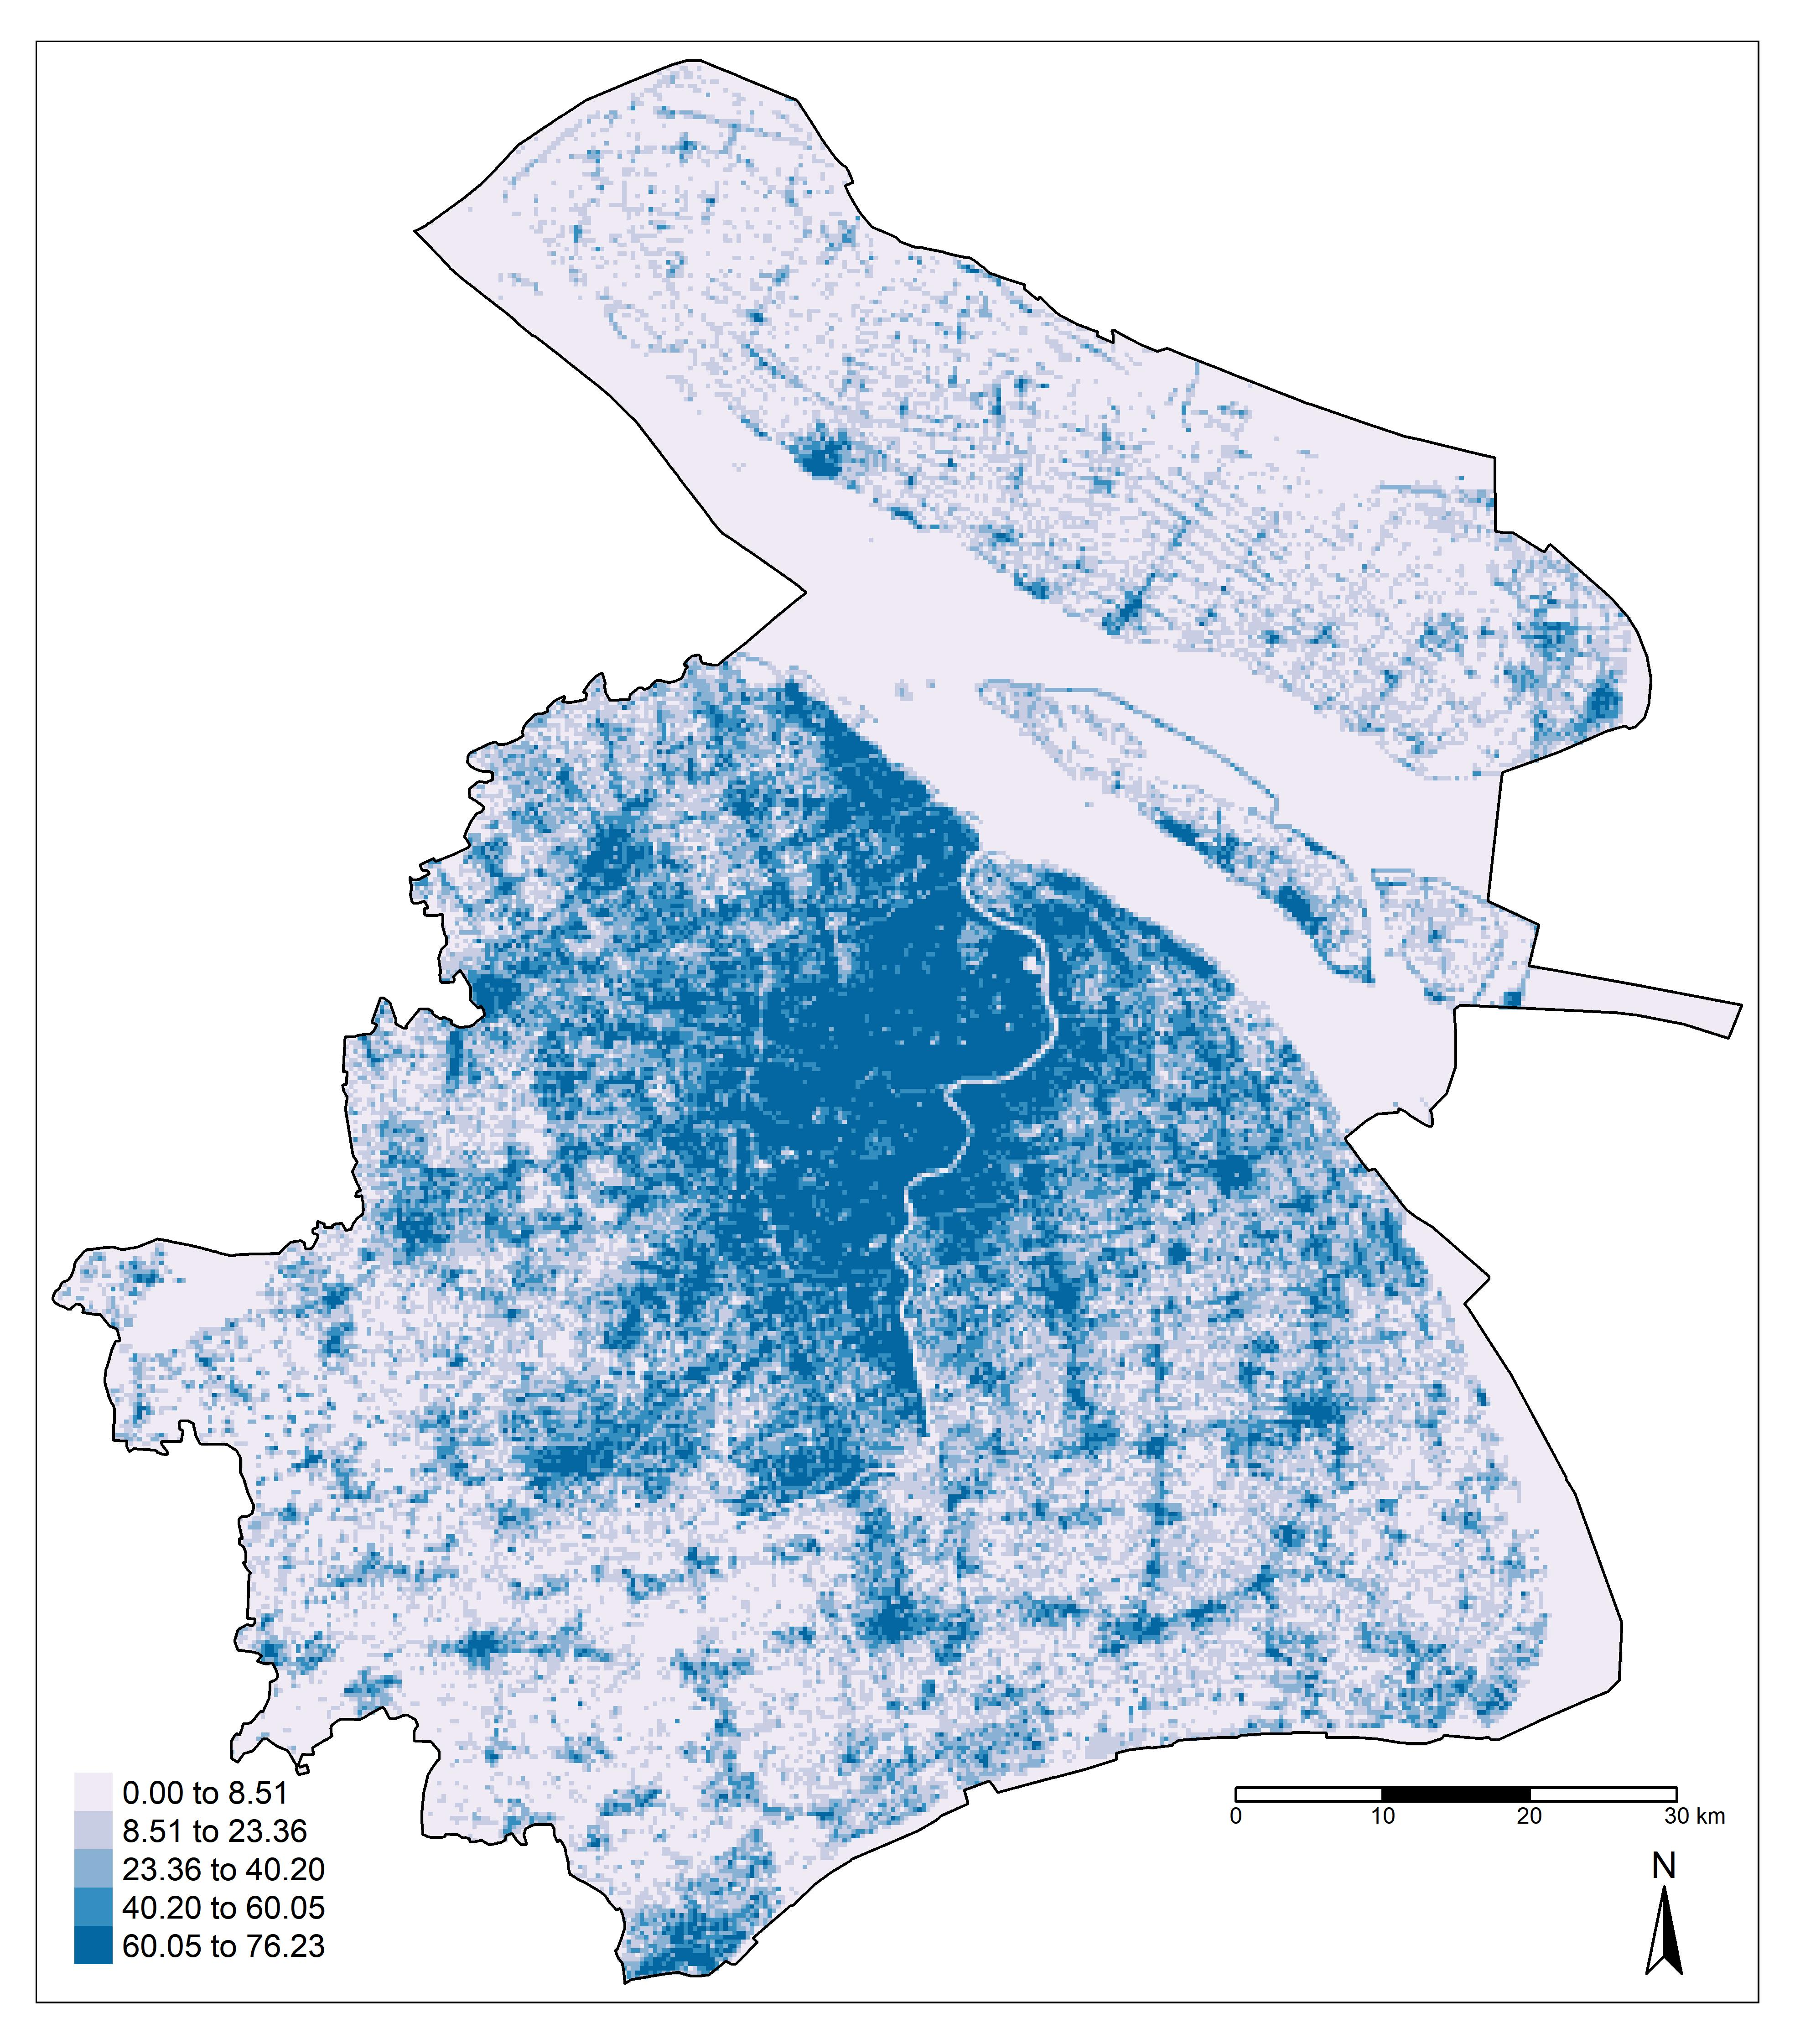
\includegraphics[width=6cm]{Figure/length_sh.jpg}
}
\quad
\subfigure[NT]{
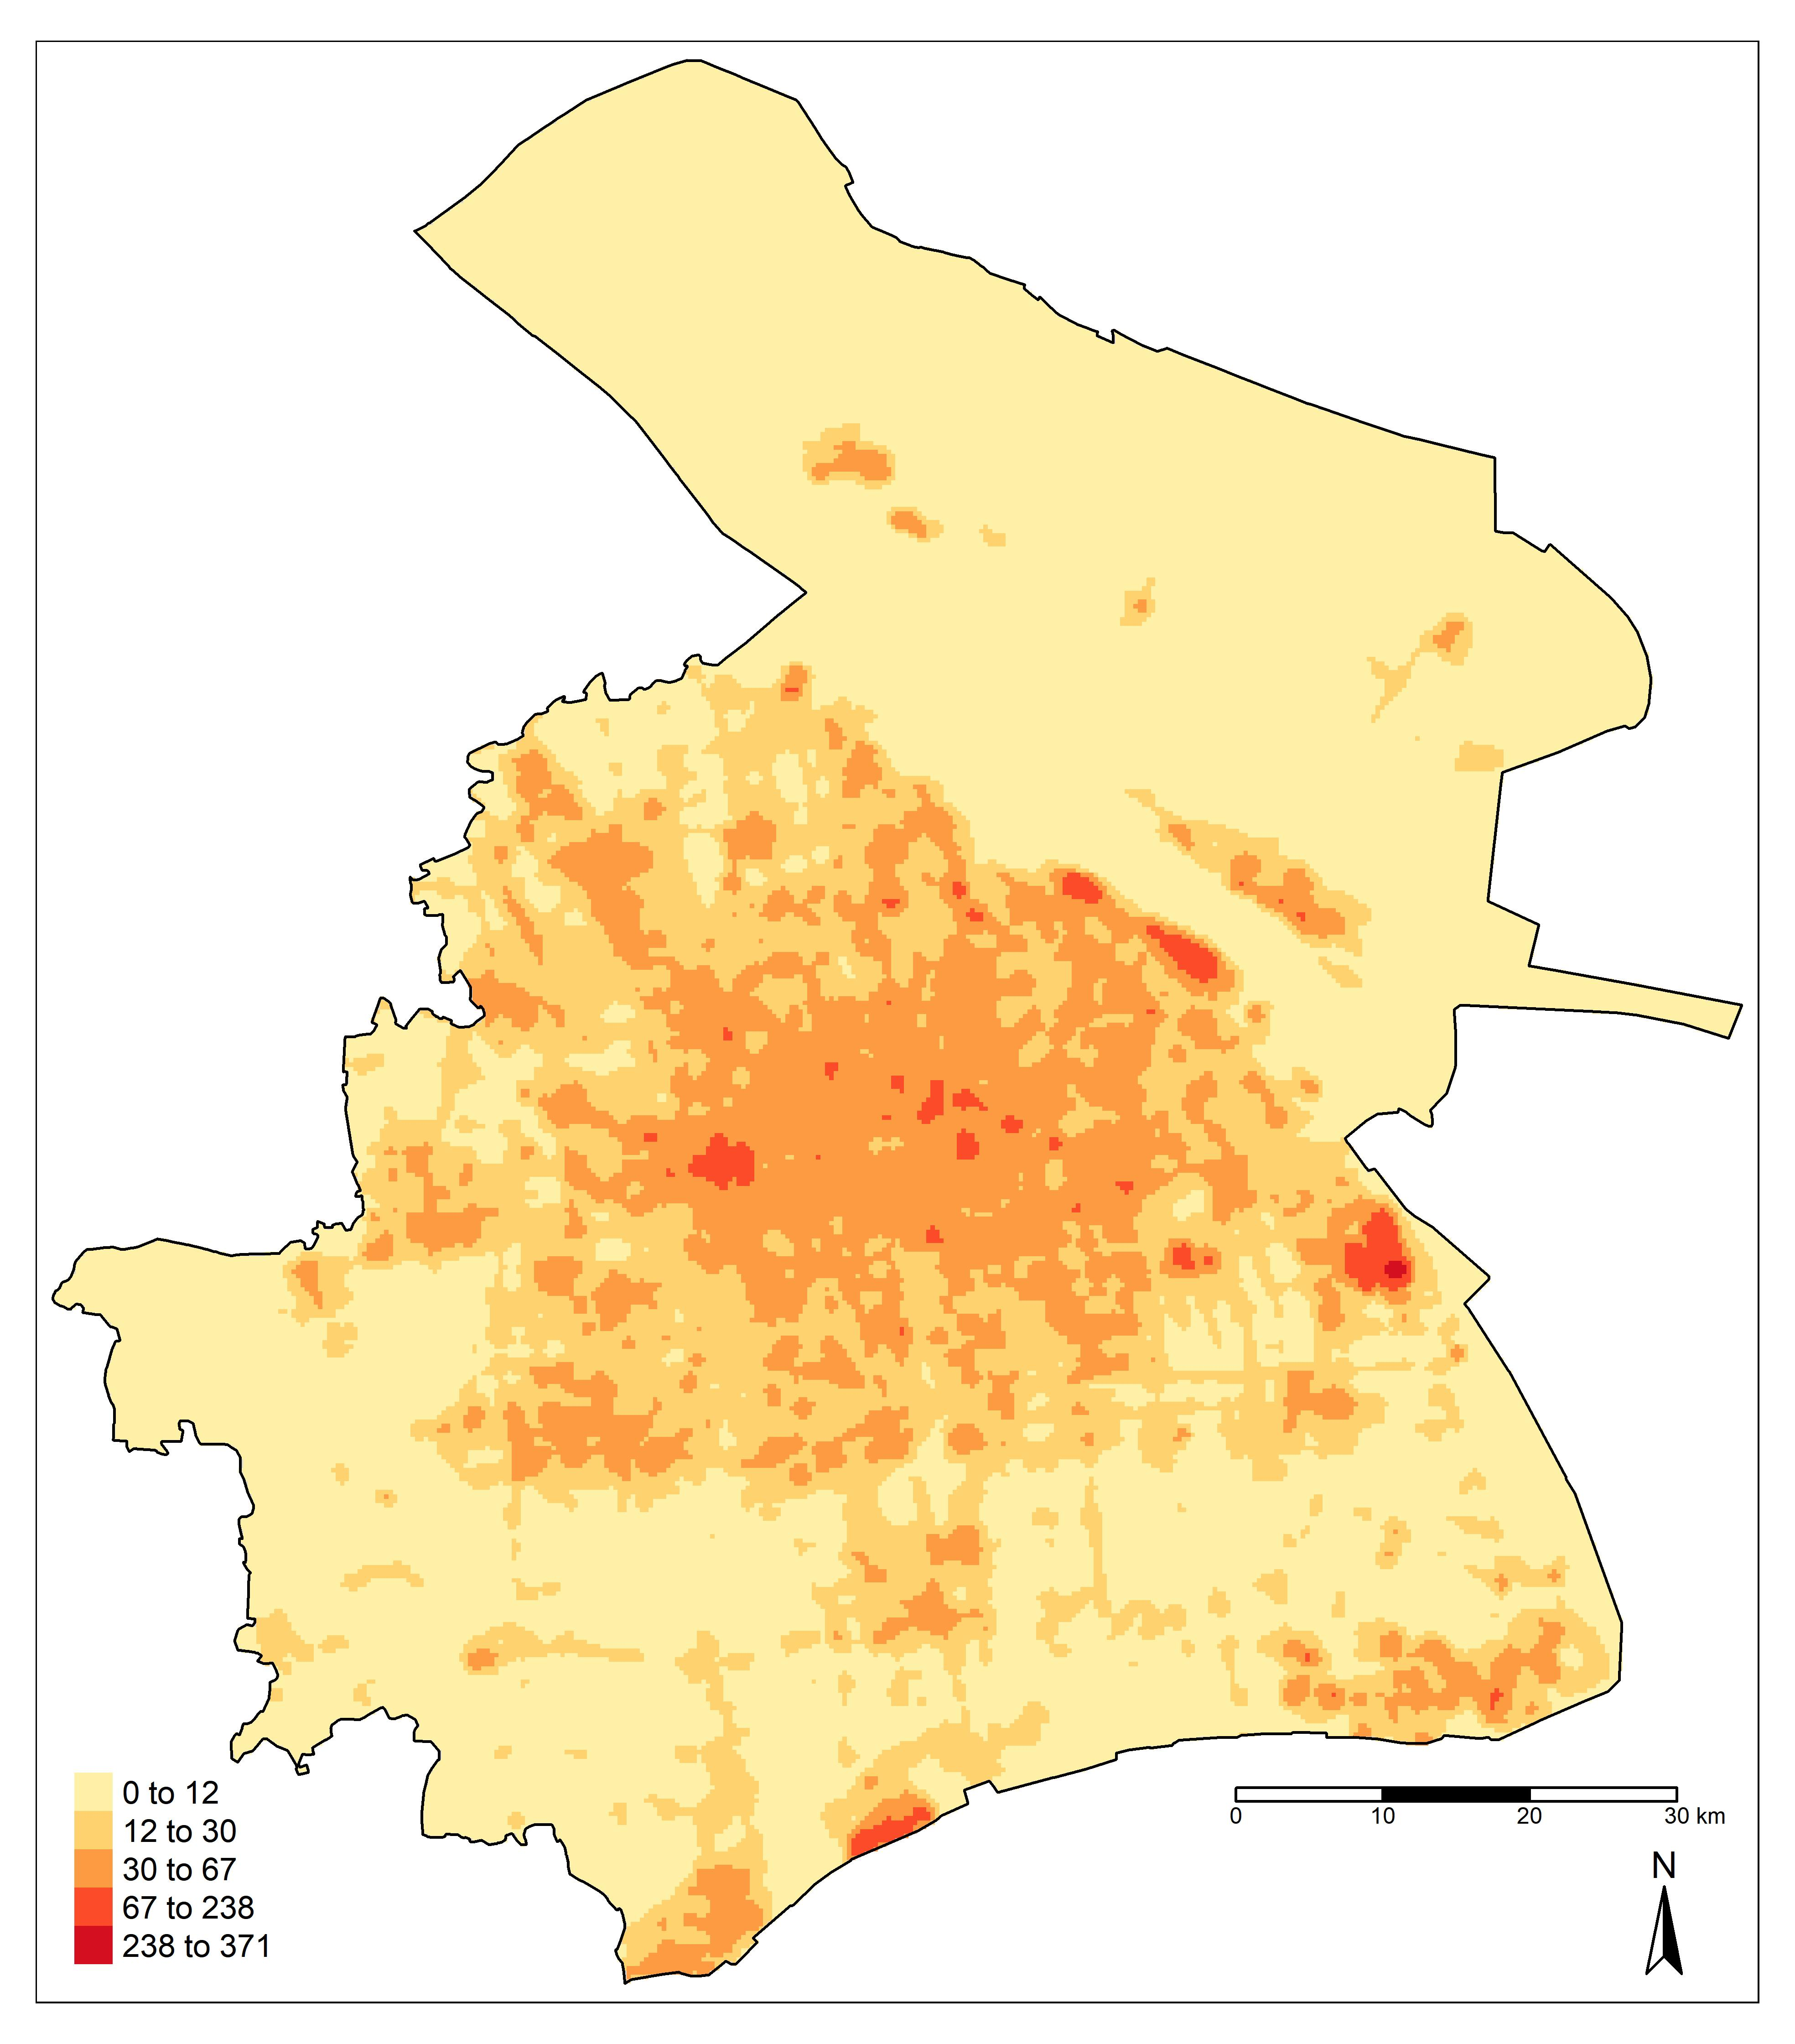
\includegraphics[width=6cm]{Figure/nt_sh.jpg}
}
\caption{Indicators of urban development system in Shanghai}
\label{ush}
\end{figure}
%%%%%%%%%%%%%%%%%%%%%%%%%%%%%%%%%%%%

\subsubsection{Urban development system indicators}
There was a distinctive feature of the NT value. When comparing with the socio-economic index, the area with high NT values were basically the same as index. Besides, NT values were mostly concentrated in the areas of construction land and farmland. In contrast to index, the highest values of NT in Guangzhou were clustered in the central northern area and the southern fringe close to the South China Sea. While the highest values in Shanghai were also partially distributed in the southern border and the eastern area close to the East China Sea. Whereas Guangzhou was compared with Shanghai, the highest value and average value of Shanghai was much larger than Guangzhou, which would further indicate that in the socio-economic development level of the city, Shanghai had a higher degree of urbanization development than Guangzhou.\\

The high-value areas in AL were mostly found in the central and southern part of Guangzhou, and the central and southern part of Shanghai. The high-value areas in AL were mostly found in the central and southern part of Guangzhou and the central and southern part of Shanghai. Compared with NT, the distribution of high-value areas from AL was more concentrated. It can be seen that the NT value remained at a low value in some areas where urban construction land was concentrated. This also showed that there were some differences in the development of construction land when it comes to development level and business potential.\\

There was some similarity between AL and CL. However, compared with AL, CL had a more uniform distribution. Especially in the central south and northwest areas of Guangzhou and the southern area of Shanghai, the high compactness areas were basically in a scattered but uniform distribution.\\



\subsubsection{Environmental index}
According to the figure Figure \ref{egz} and \ref{esh}, The high-values of environmental index in Guangzhou were mainly concentrated in the mountainous and woodland areas in the northern part of the city. In terms of the spatial layout of Guangzhou, some of the areas with the highest values were mostly close to the urban boundary areas. This may be due to the relatively low level of development and fewer traces of human activities in the border areas. Some of the smaller high-value patches were evenly distributed in the central area of the northern part of the city, which also undertook part of the energy transfer function of the ecological source sites in the northern area. This phenomenon also maintained a stable ecological function in the north side.\\

The index values in the southern part of the city were generally in the medium level. The distribution of high-value areas in the area was more fragmented and there was not a concentrated cluster of patches. This may be due to the relatively low environmental outcome caused by the southward expansion of the city. At the same time, the interspersed distribution of urban construction land led to the fragmentation of large ecological patches.\\

Moreover, The lowest index values were found in the middle of the city. This could also be attributed to the relatively high degree of urban construction in the area. The ecological index of the urban area was also significantly lower.\\

When it comes to Shanghai, there were significant differences between the urban construction land and the non-urban construction areas of the environmental index. In terms of the spatial layout of the area in Shanghai, the index value of construction land in the middle of the city was relatively low. However, the distribution of high-value areas in the surrounding areas of the city was uniformly distributed. There was no uniform concentration of large patches in this type of area, but the high-value areas were evenly interspersed into the medium and low-value areas. This also formed an external ecological network.\\

Compared with Guangzhou, the spatial layout of Shanghai was significantly different. The ecological high-value areas in Guangzhou were concentrated and distributed, while the ecological high-value areas in Shanghai were evenly interspersed.\\

%%%%%%%%%%%%%%%%%%%%%%%%%%%%%%%%%%%%
\begin{figure}[H]
\centering
\subfigure[Environmental index]{
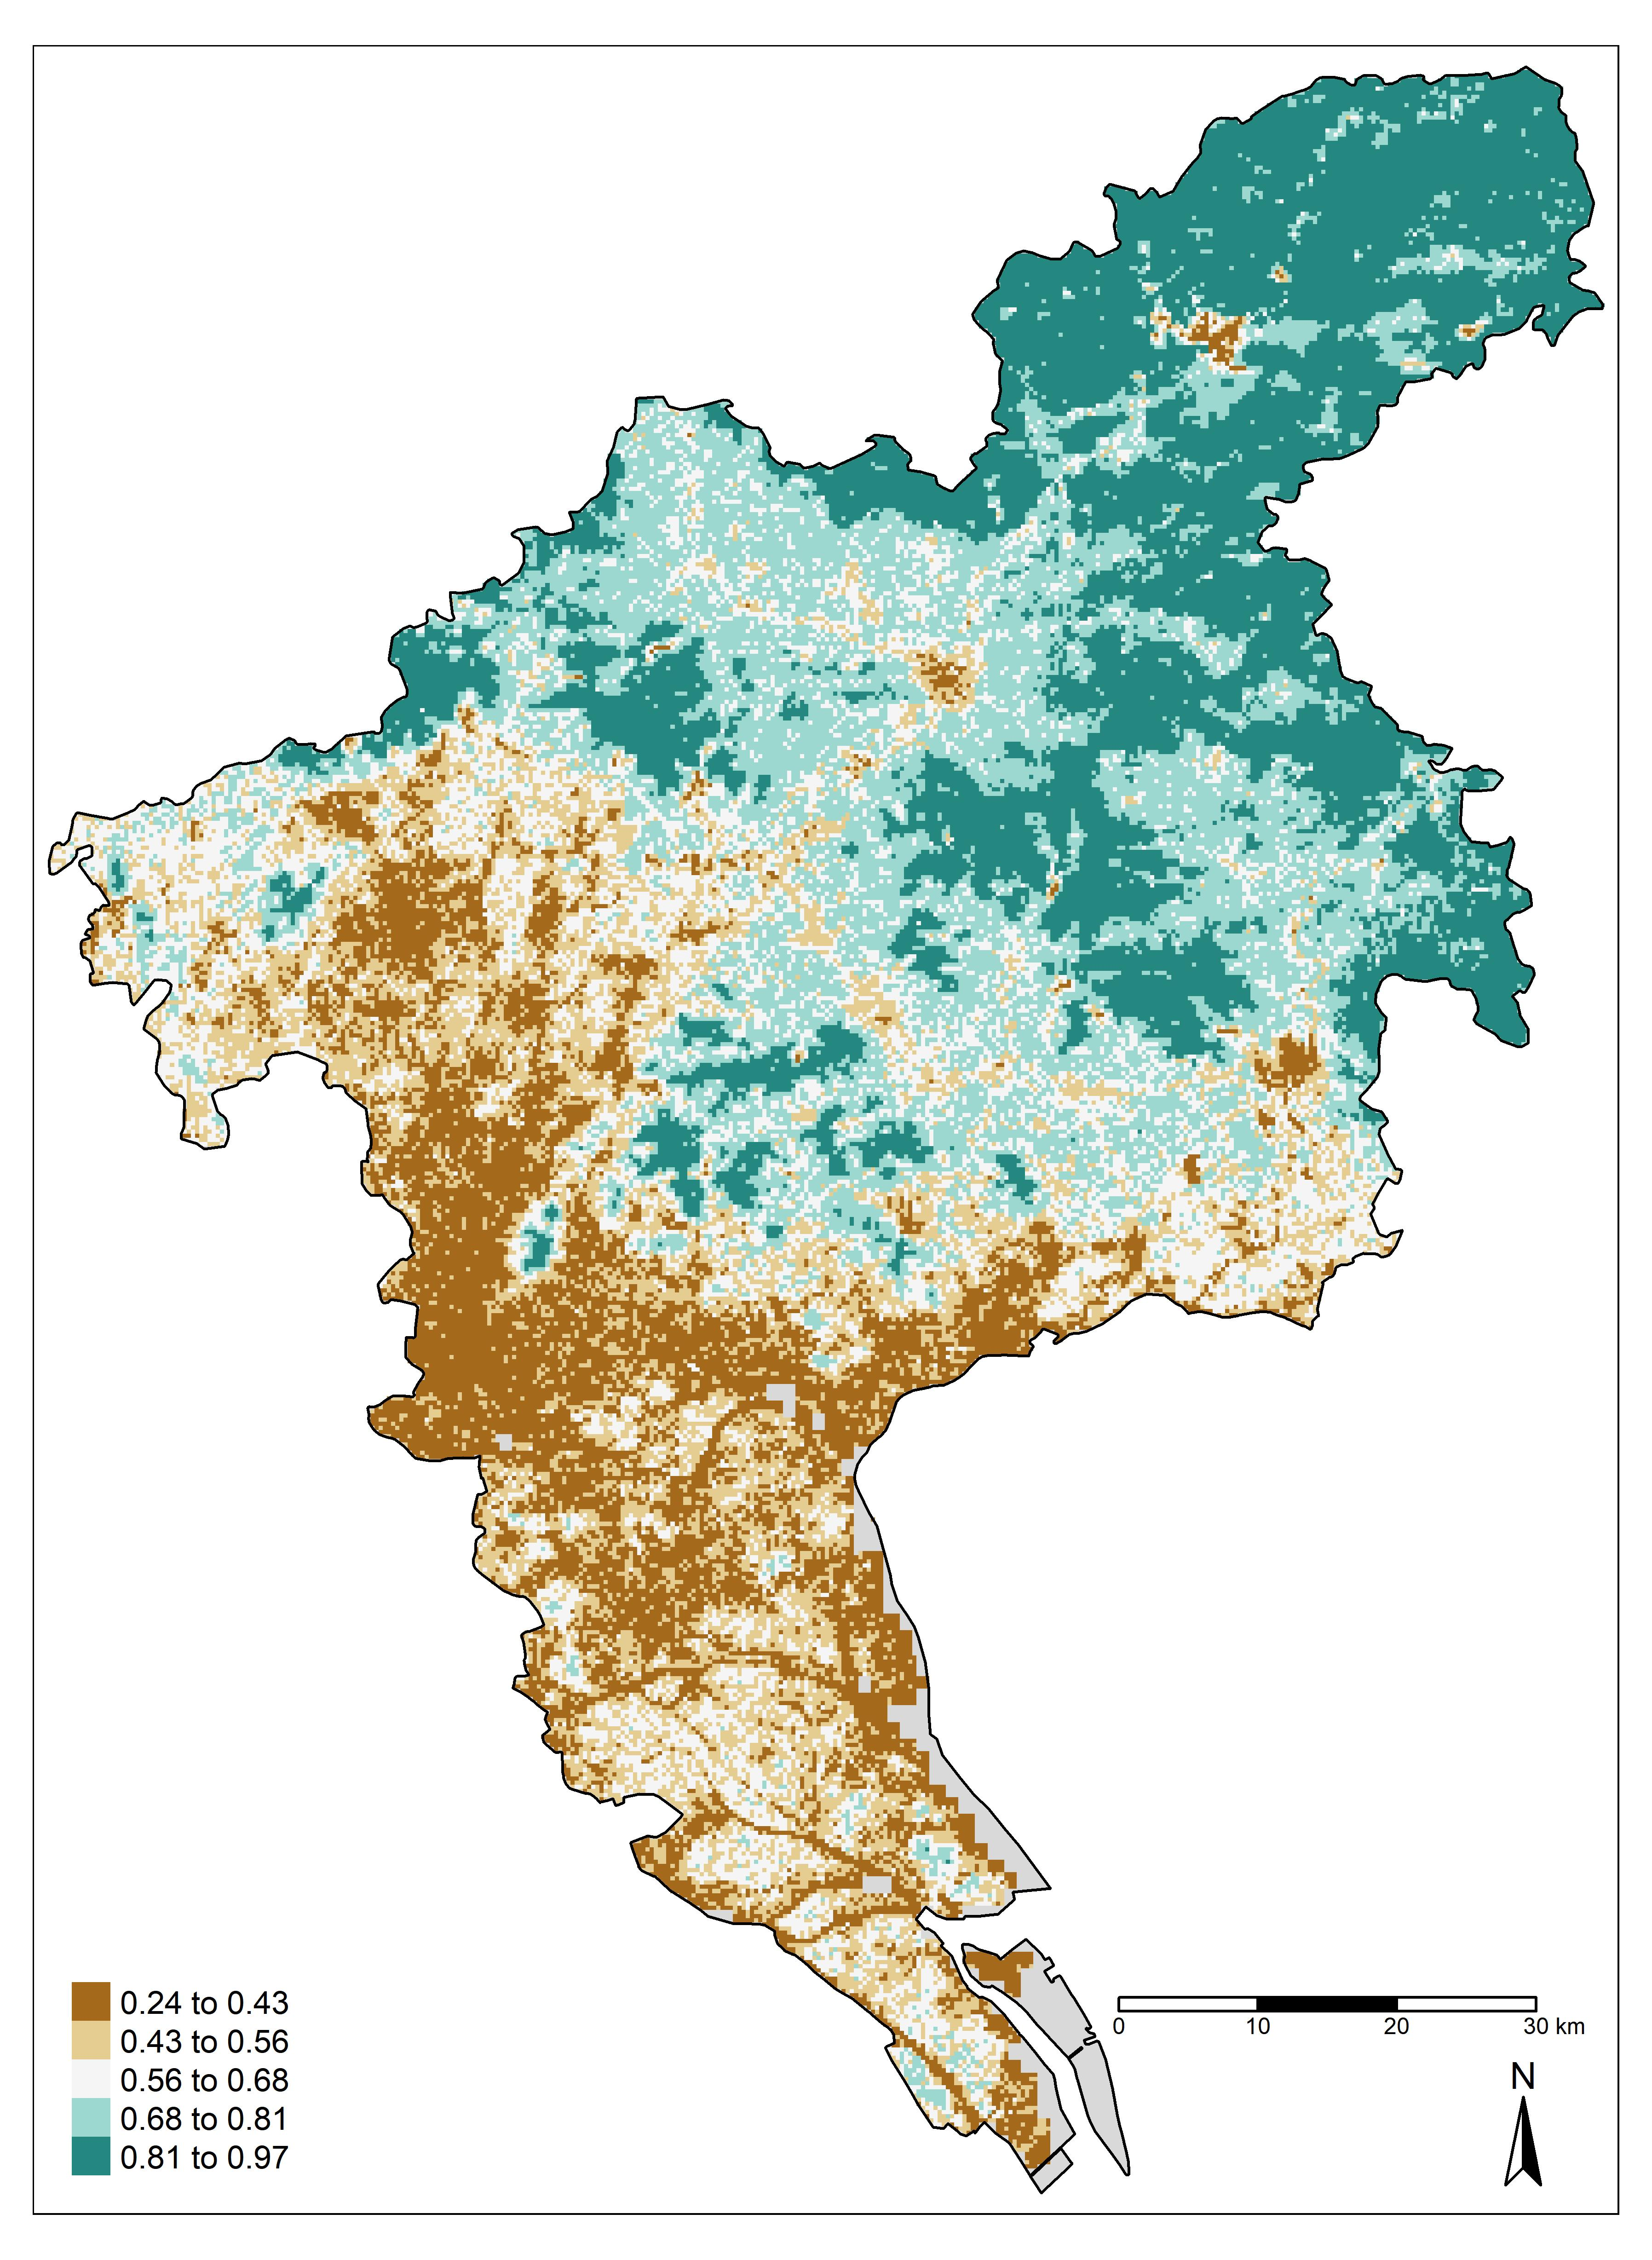
\includegraphics[width=6cm]{Figure/egz.jpg}
}
\quad
\subfigure[NDVI]{
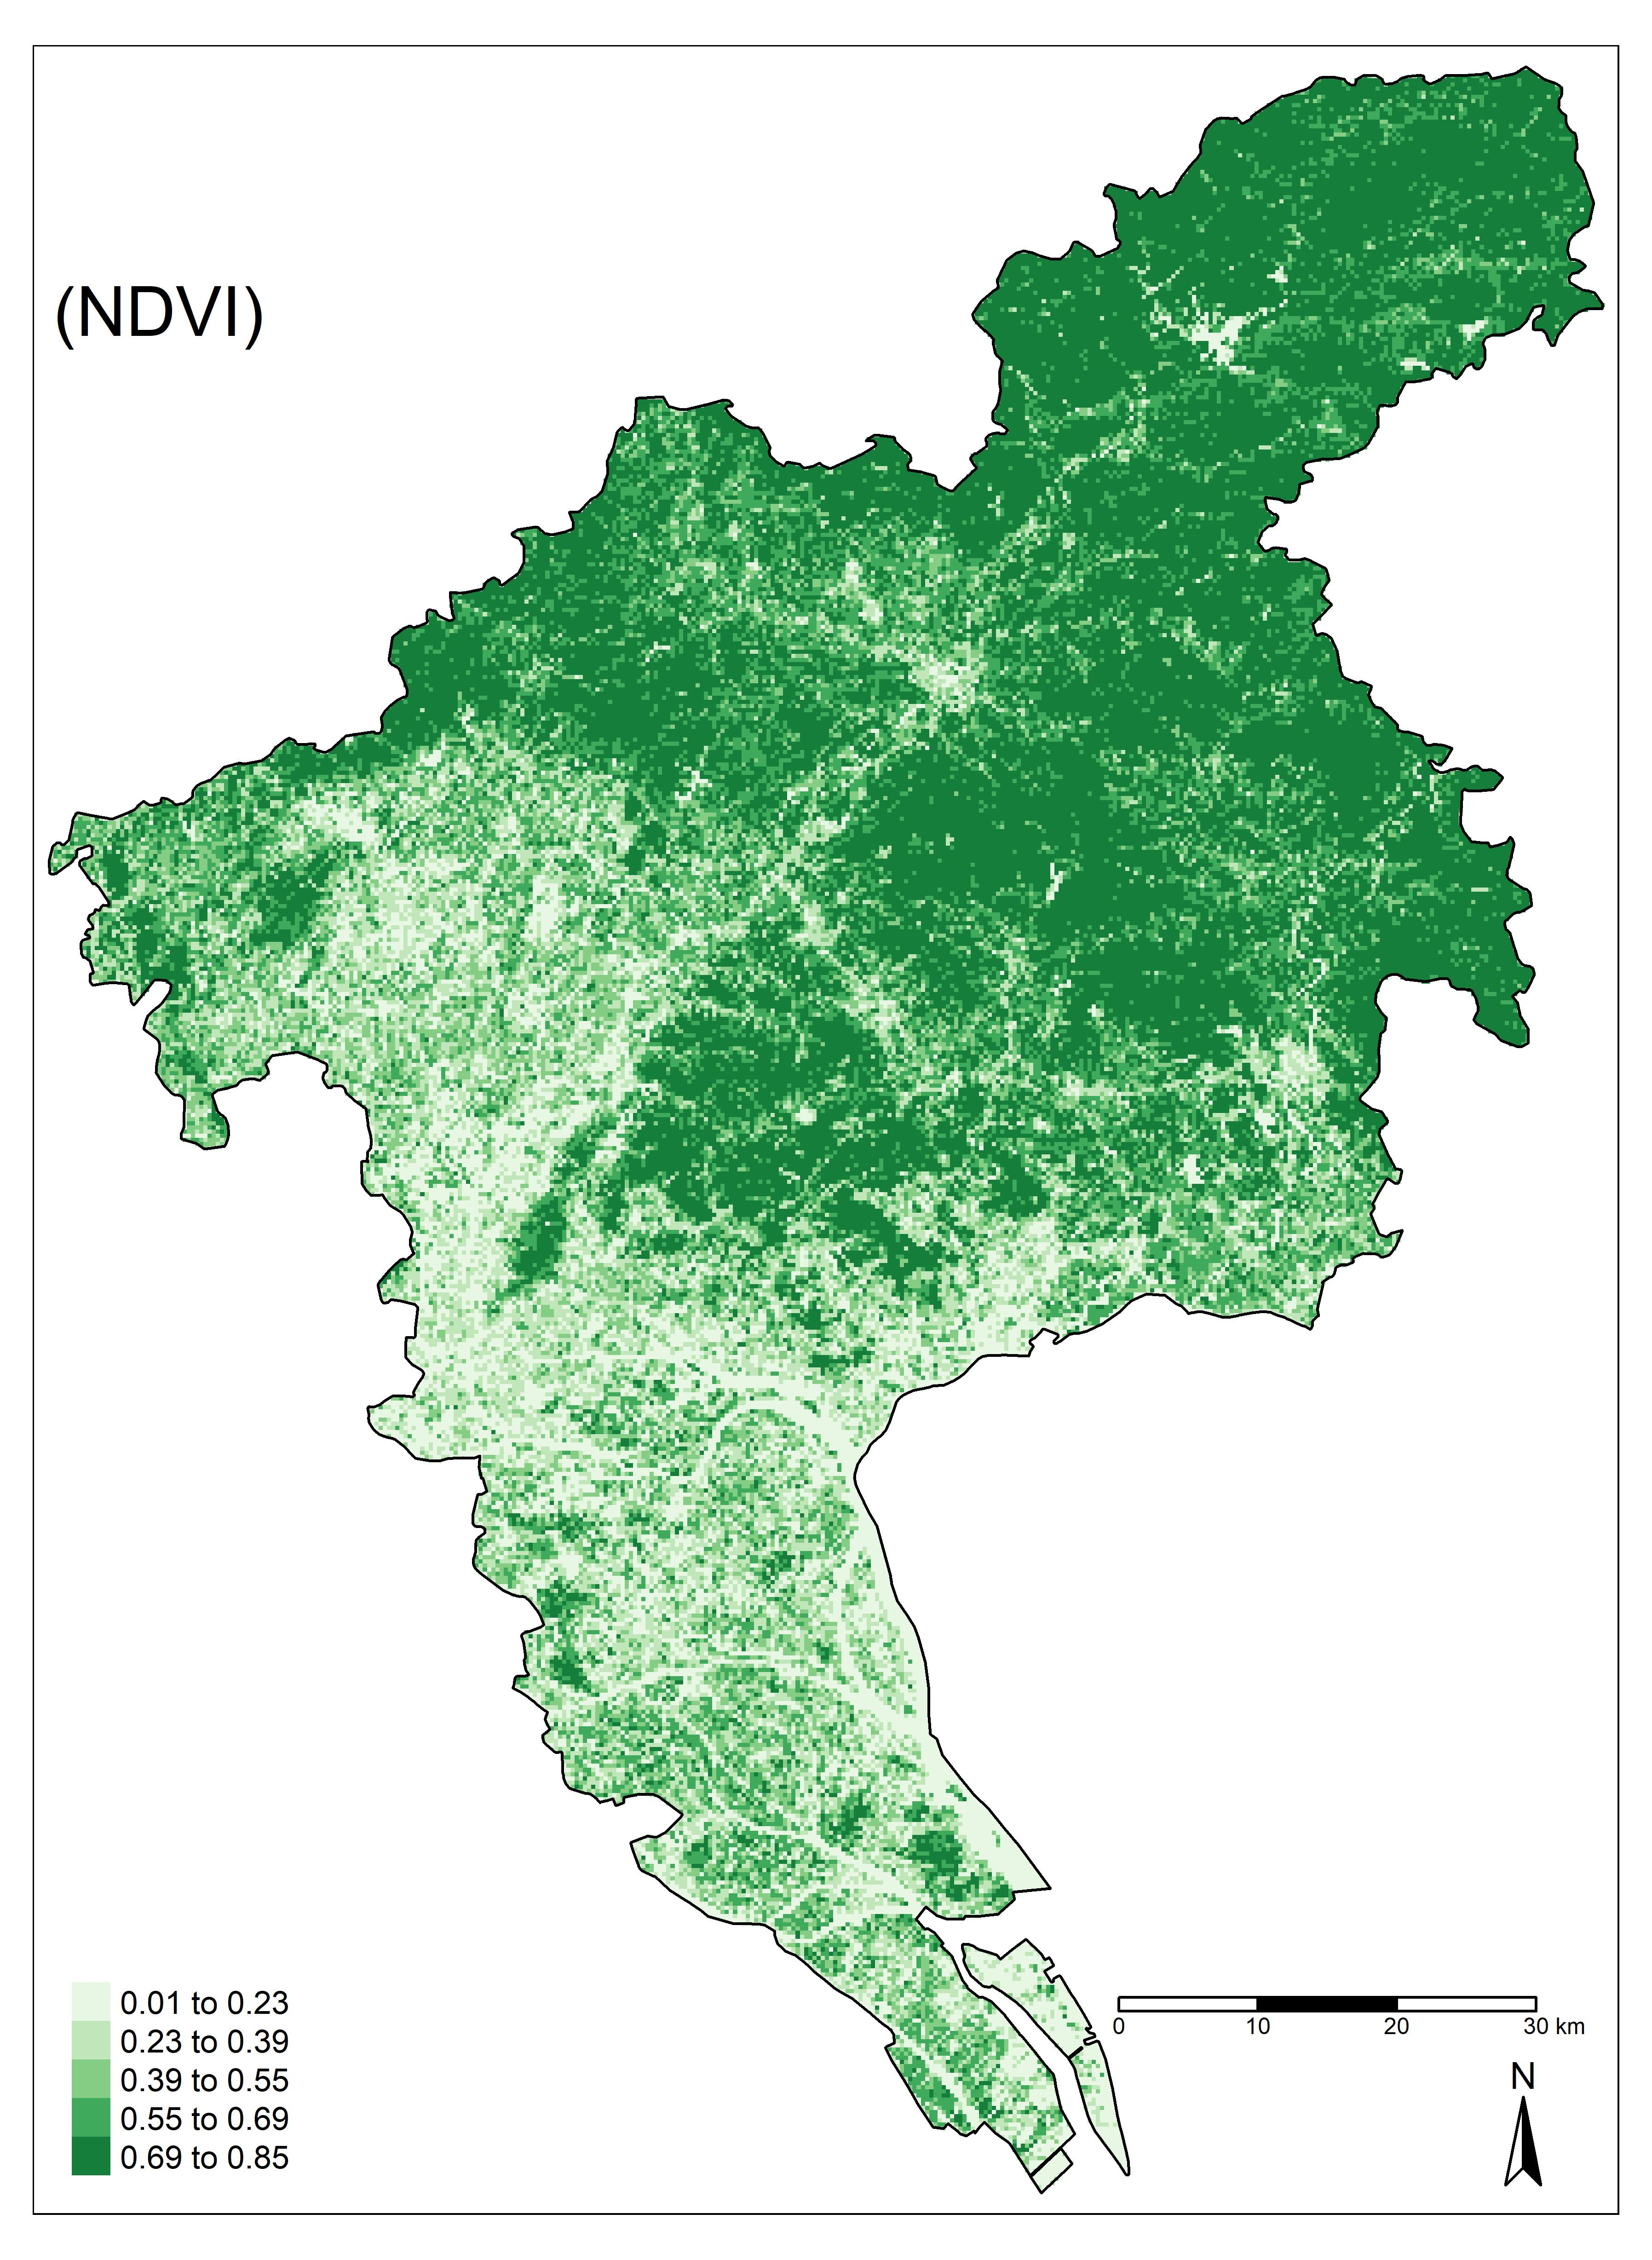
\includegraphics[width=6cm]{Figure/ndvi_gz.jpg}
}
\quad
\subfigure[NPP]{
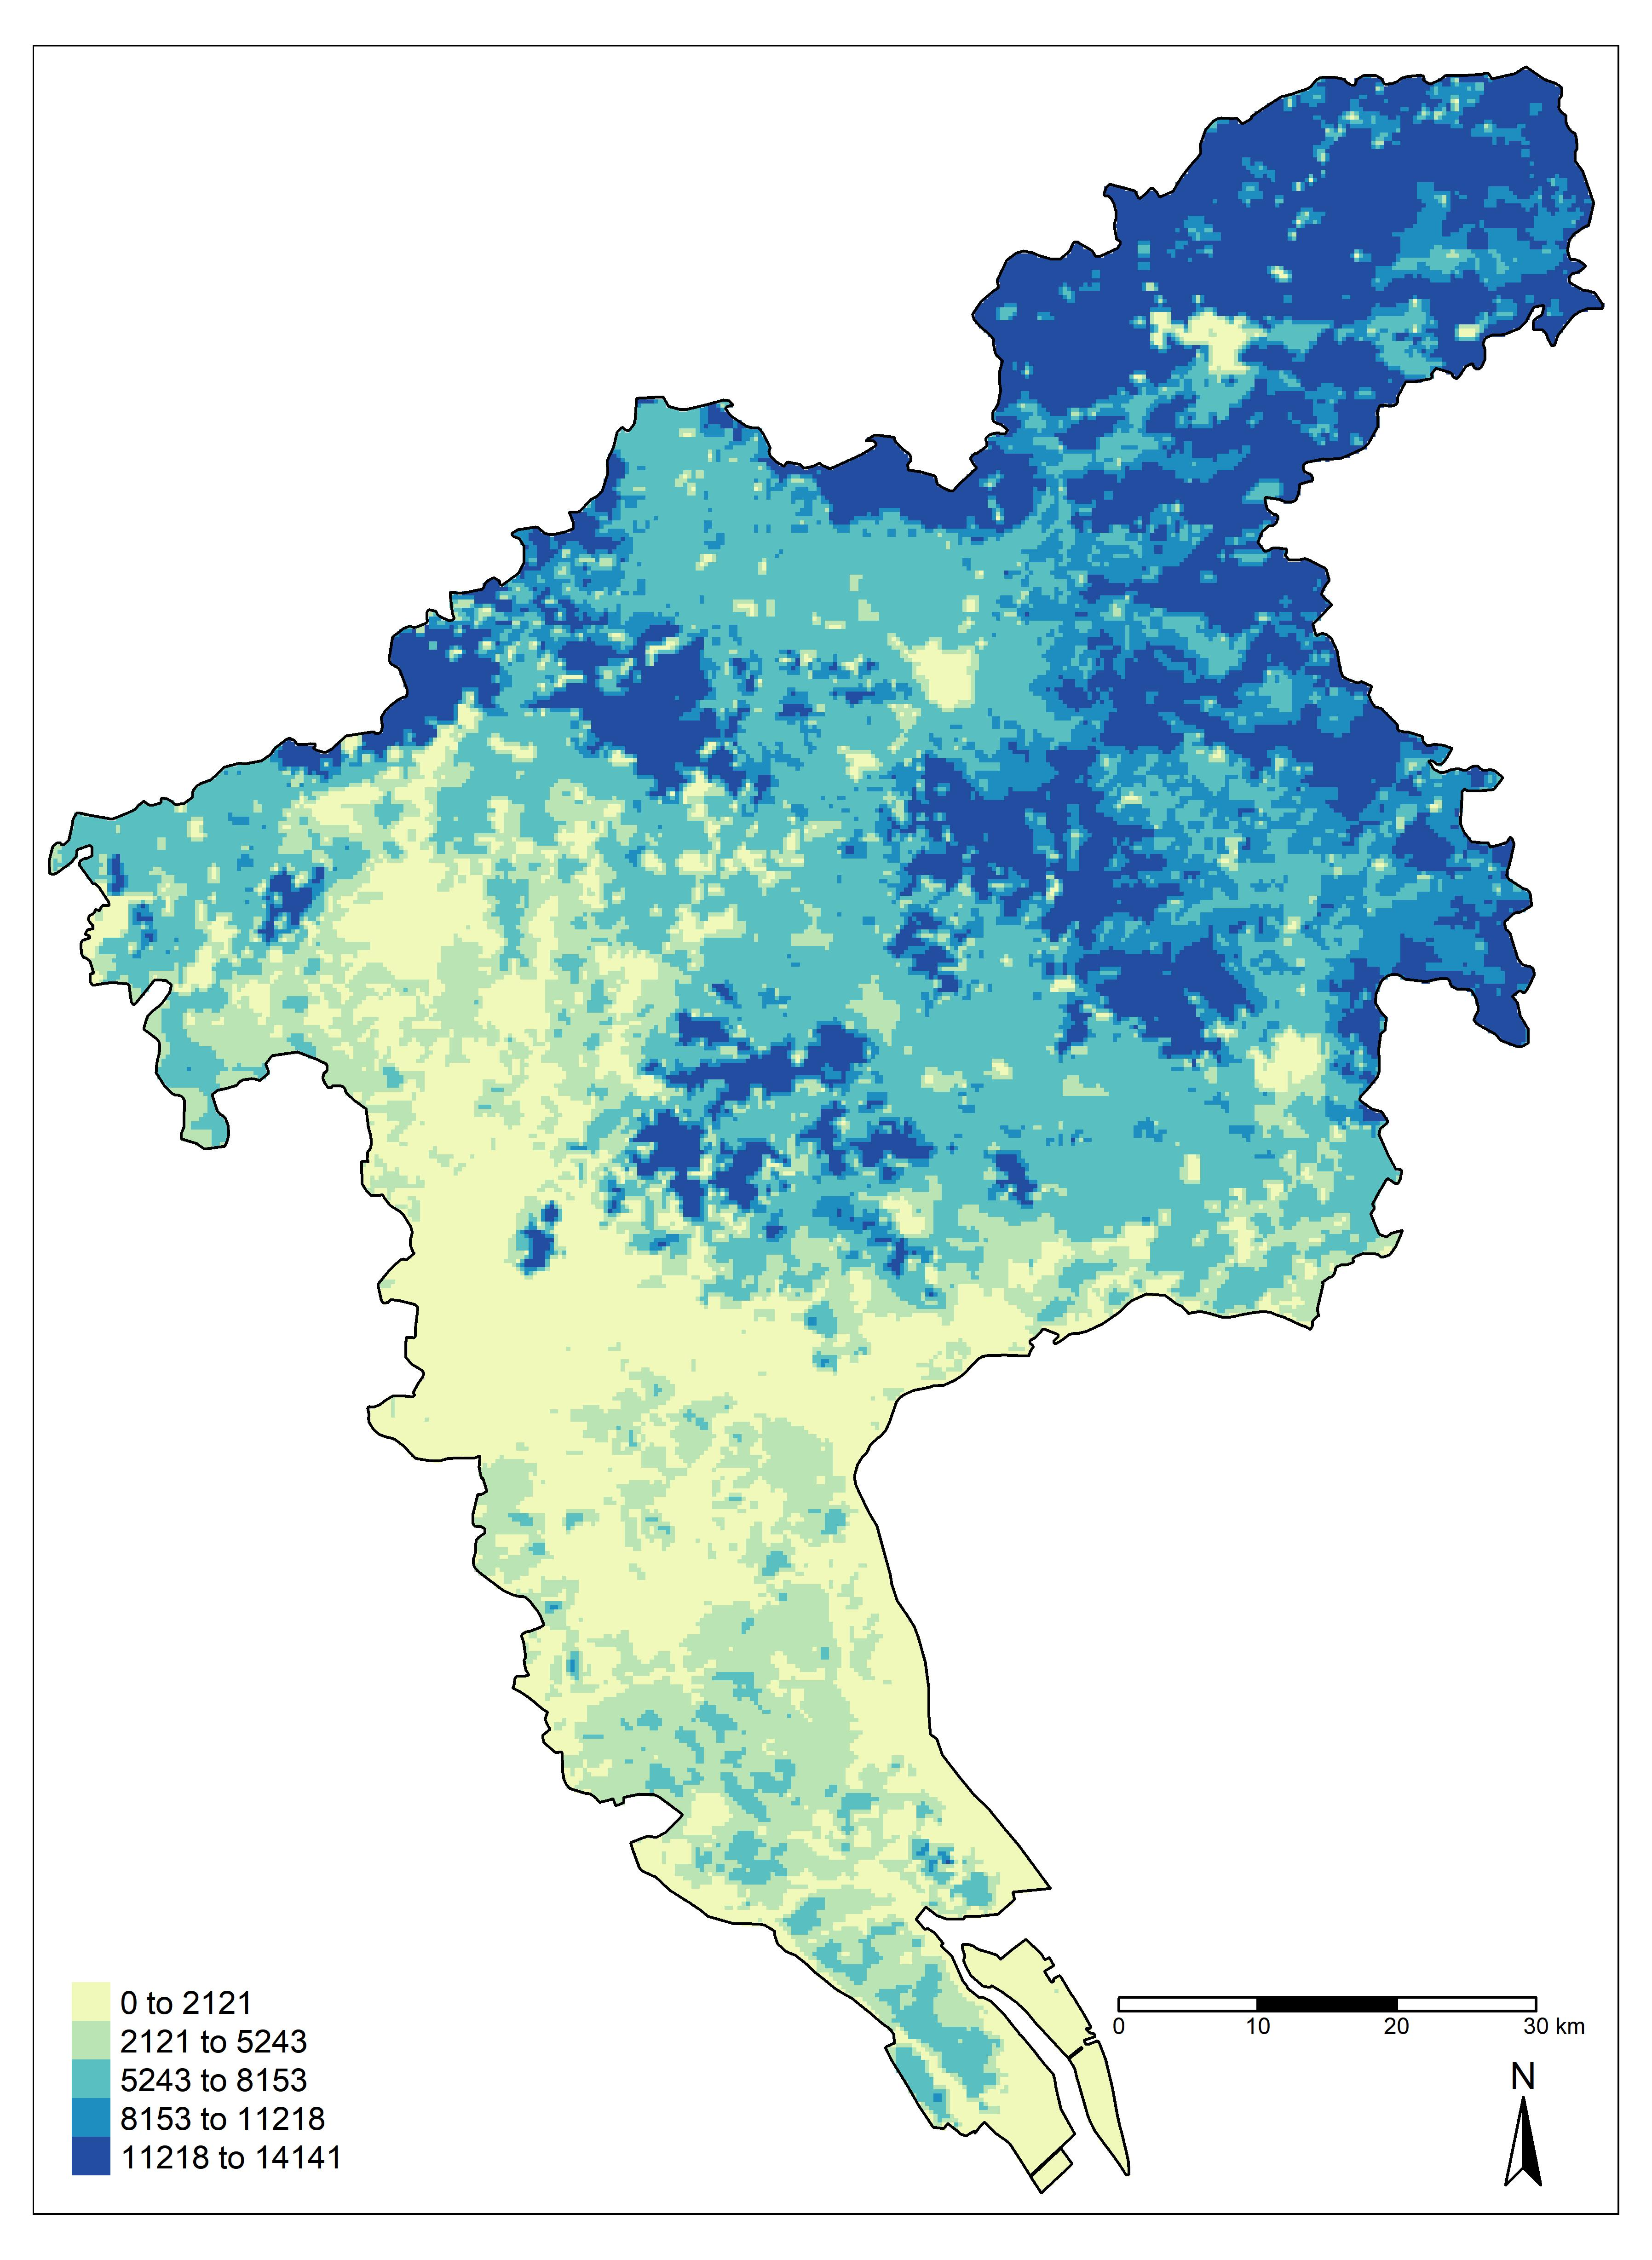
\includegraphics[width=6cm]{Figure/npp_gz.jpg}
}
\quad
\subfigure[PM2.5]{
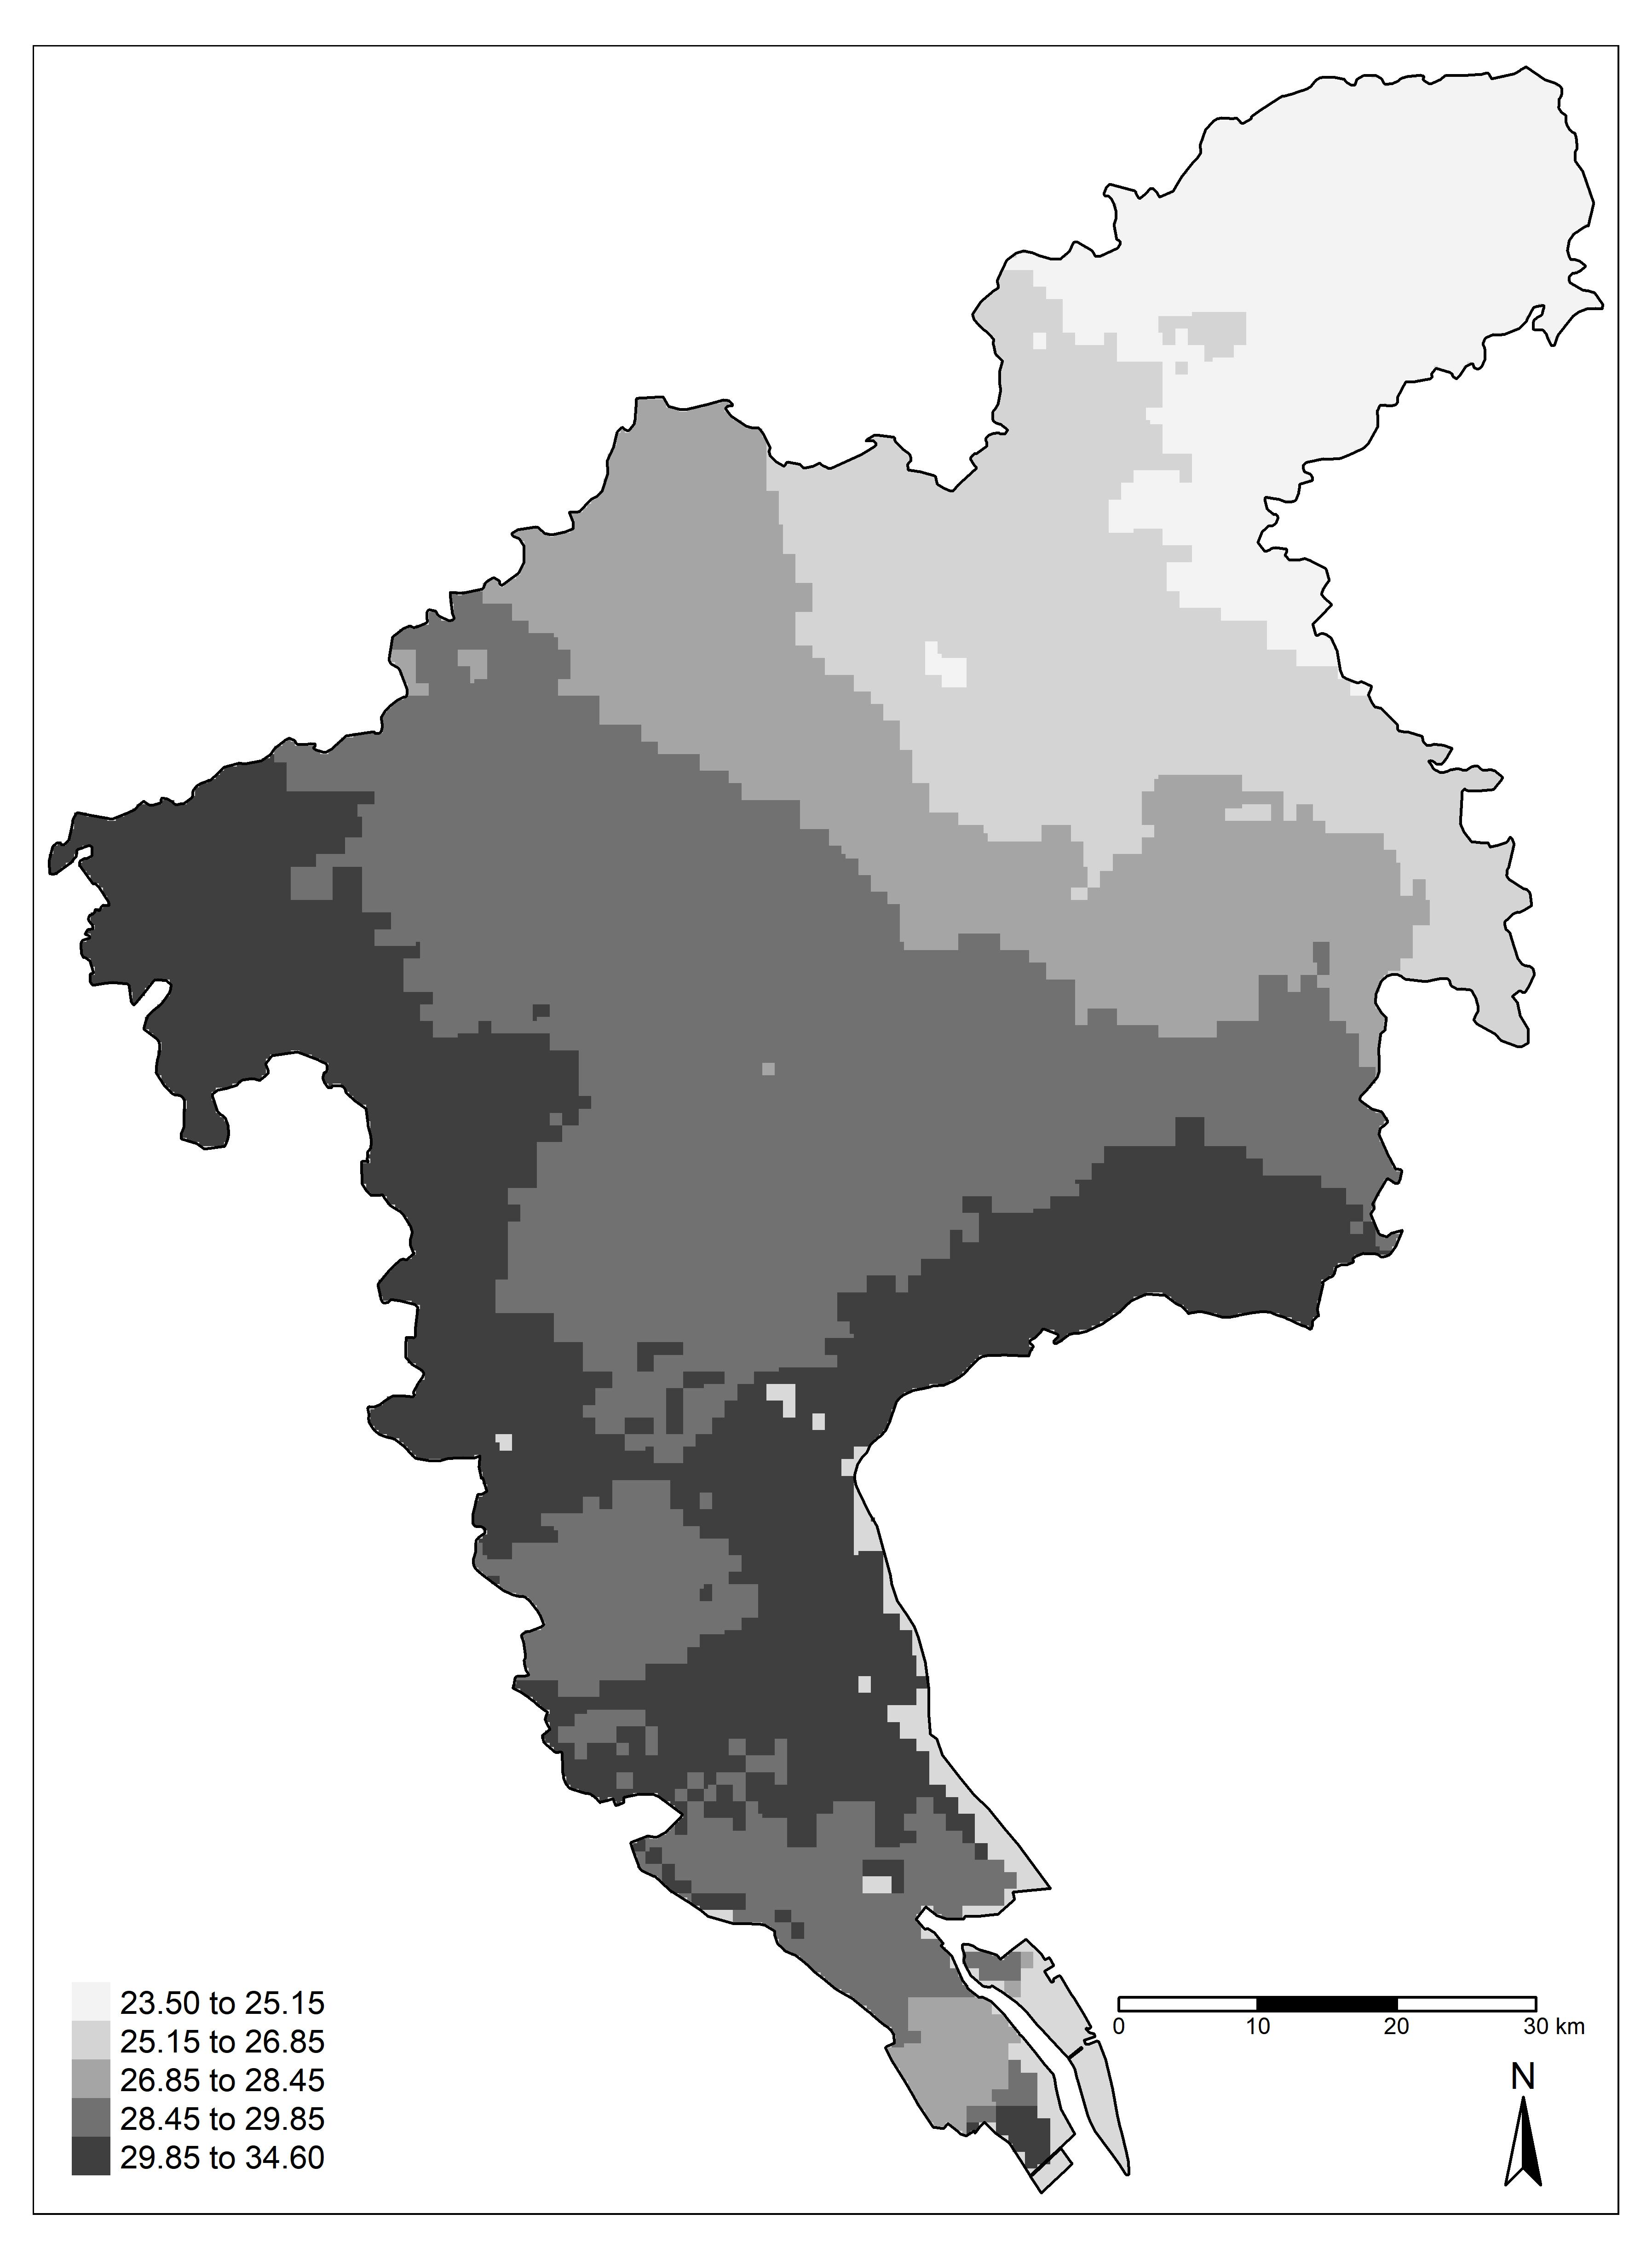
\includegraphics[width=6cm]{Figure/pm_gz.jpg}
}
\caption{Indicators of environmental system in Guangzhou}
\label{egz}
\end{figure}
%%%%%%%%%%%%%%%%%%%%%%%%%%%%%%%%%%%%

%%%%%%%%%%%%%%%%%%%%%%%%%%%%%%%%%%%%
\begin{figure}[H]
\centering
\subfigure[Environmental index]{
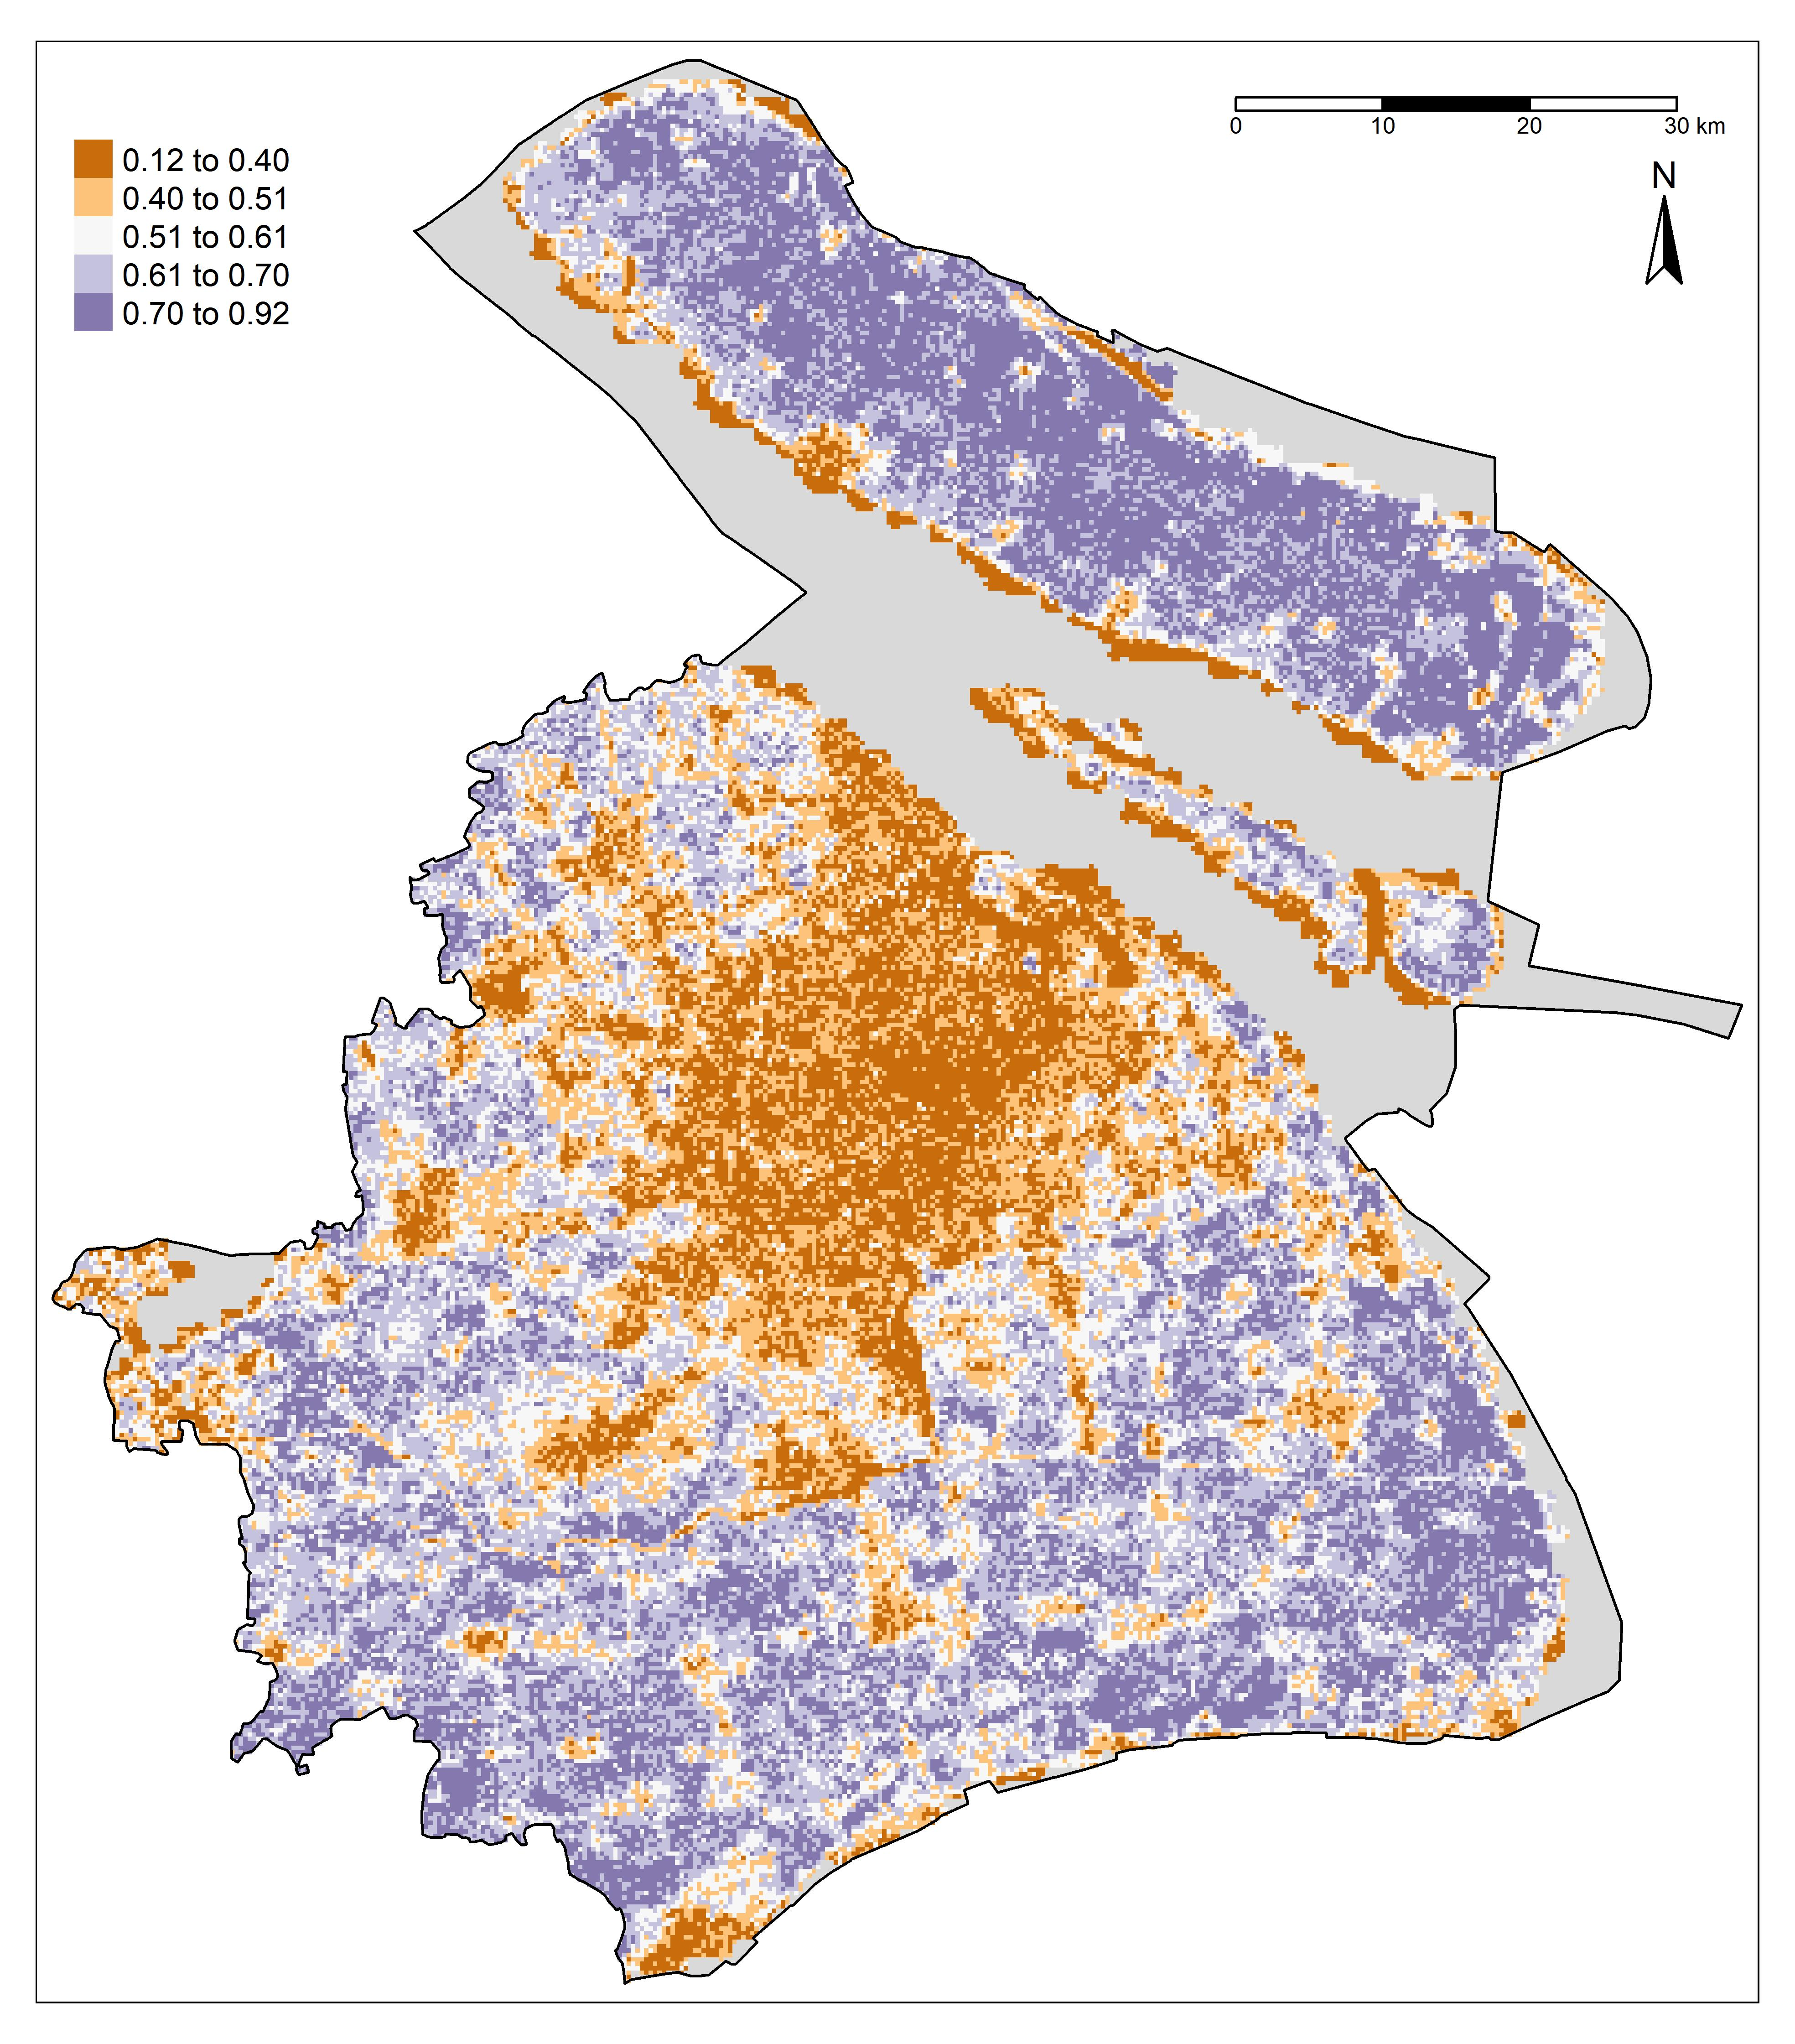
\includegraphics[width=6cm]{Figure/esh.jpg}
}
\quad
\subfigure[NDVI]{
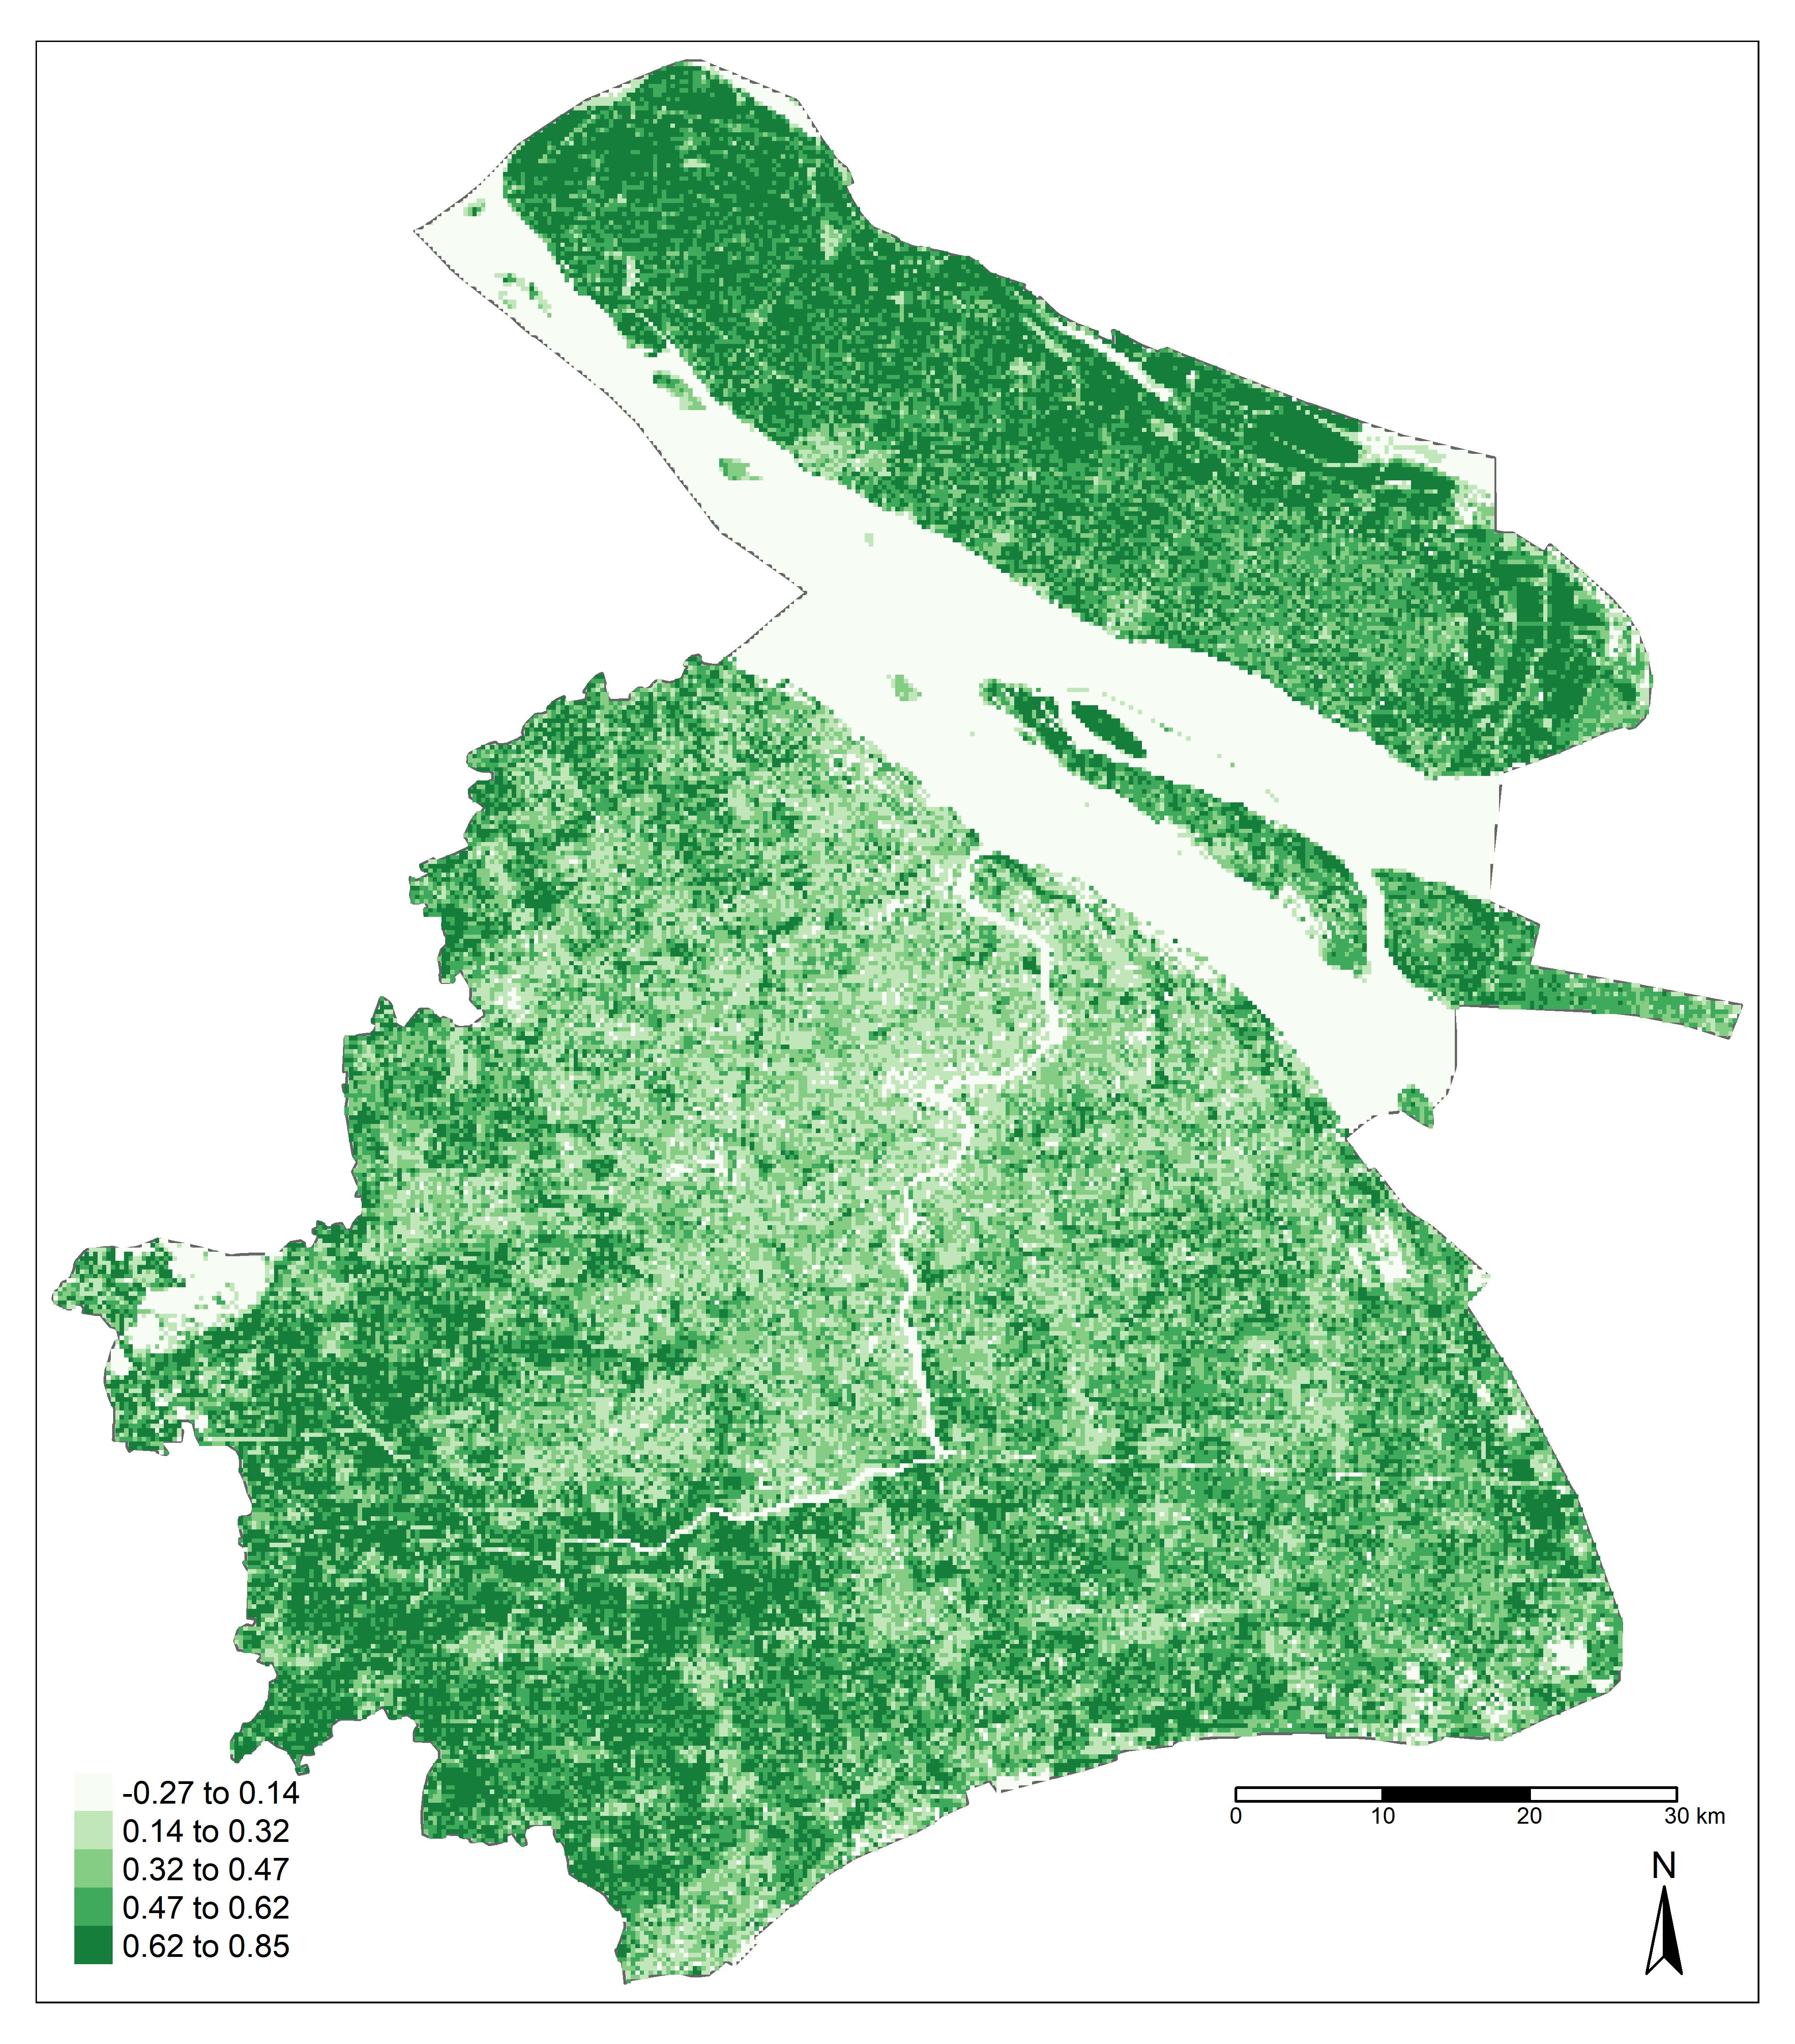
\includegraphics[width=6cm]{Figure/ndvi_sh.jpg}
}
\quad
\subfigure[NPP]{
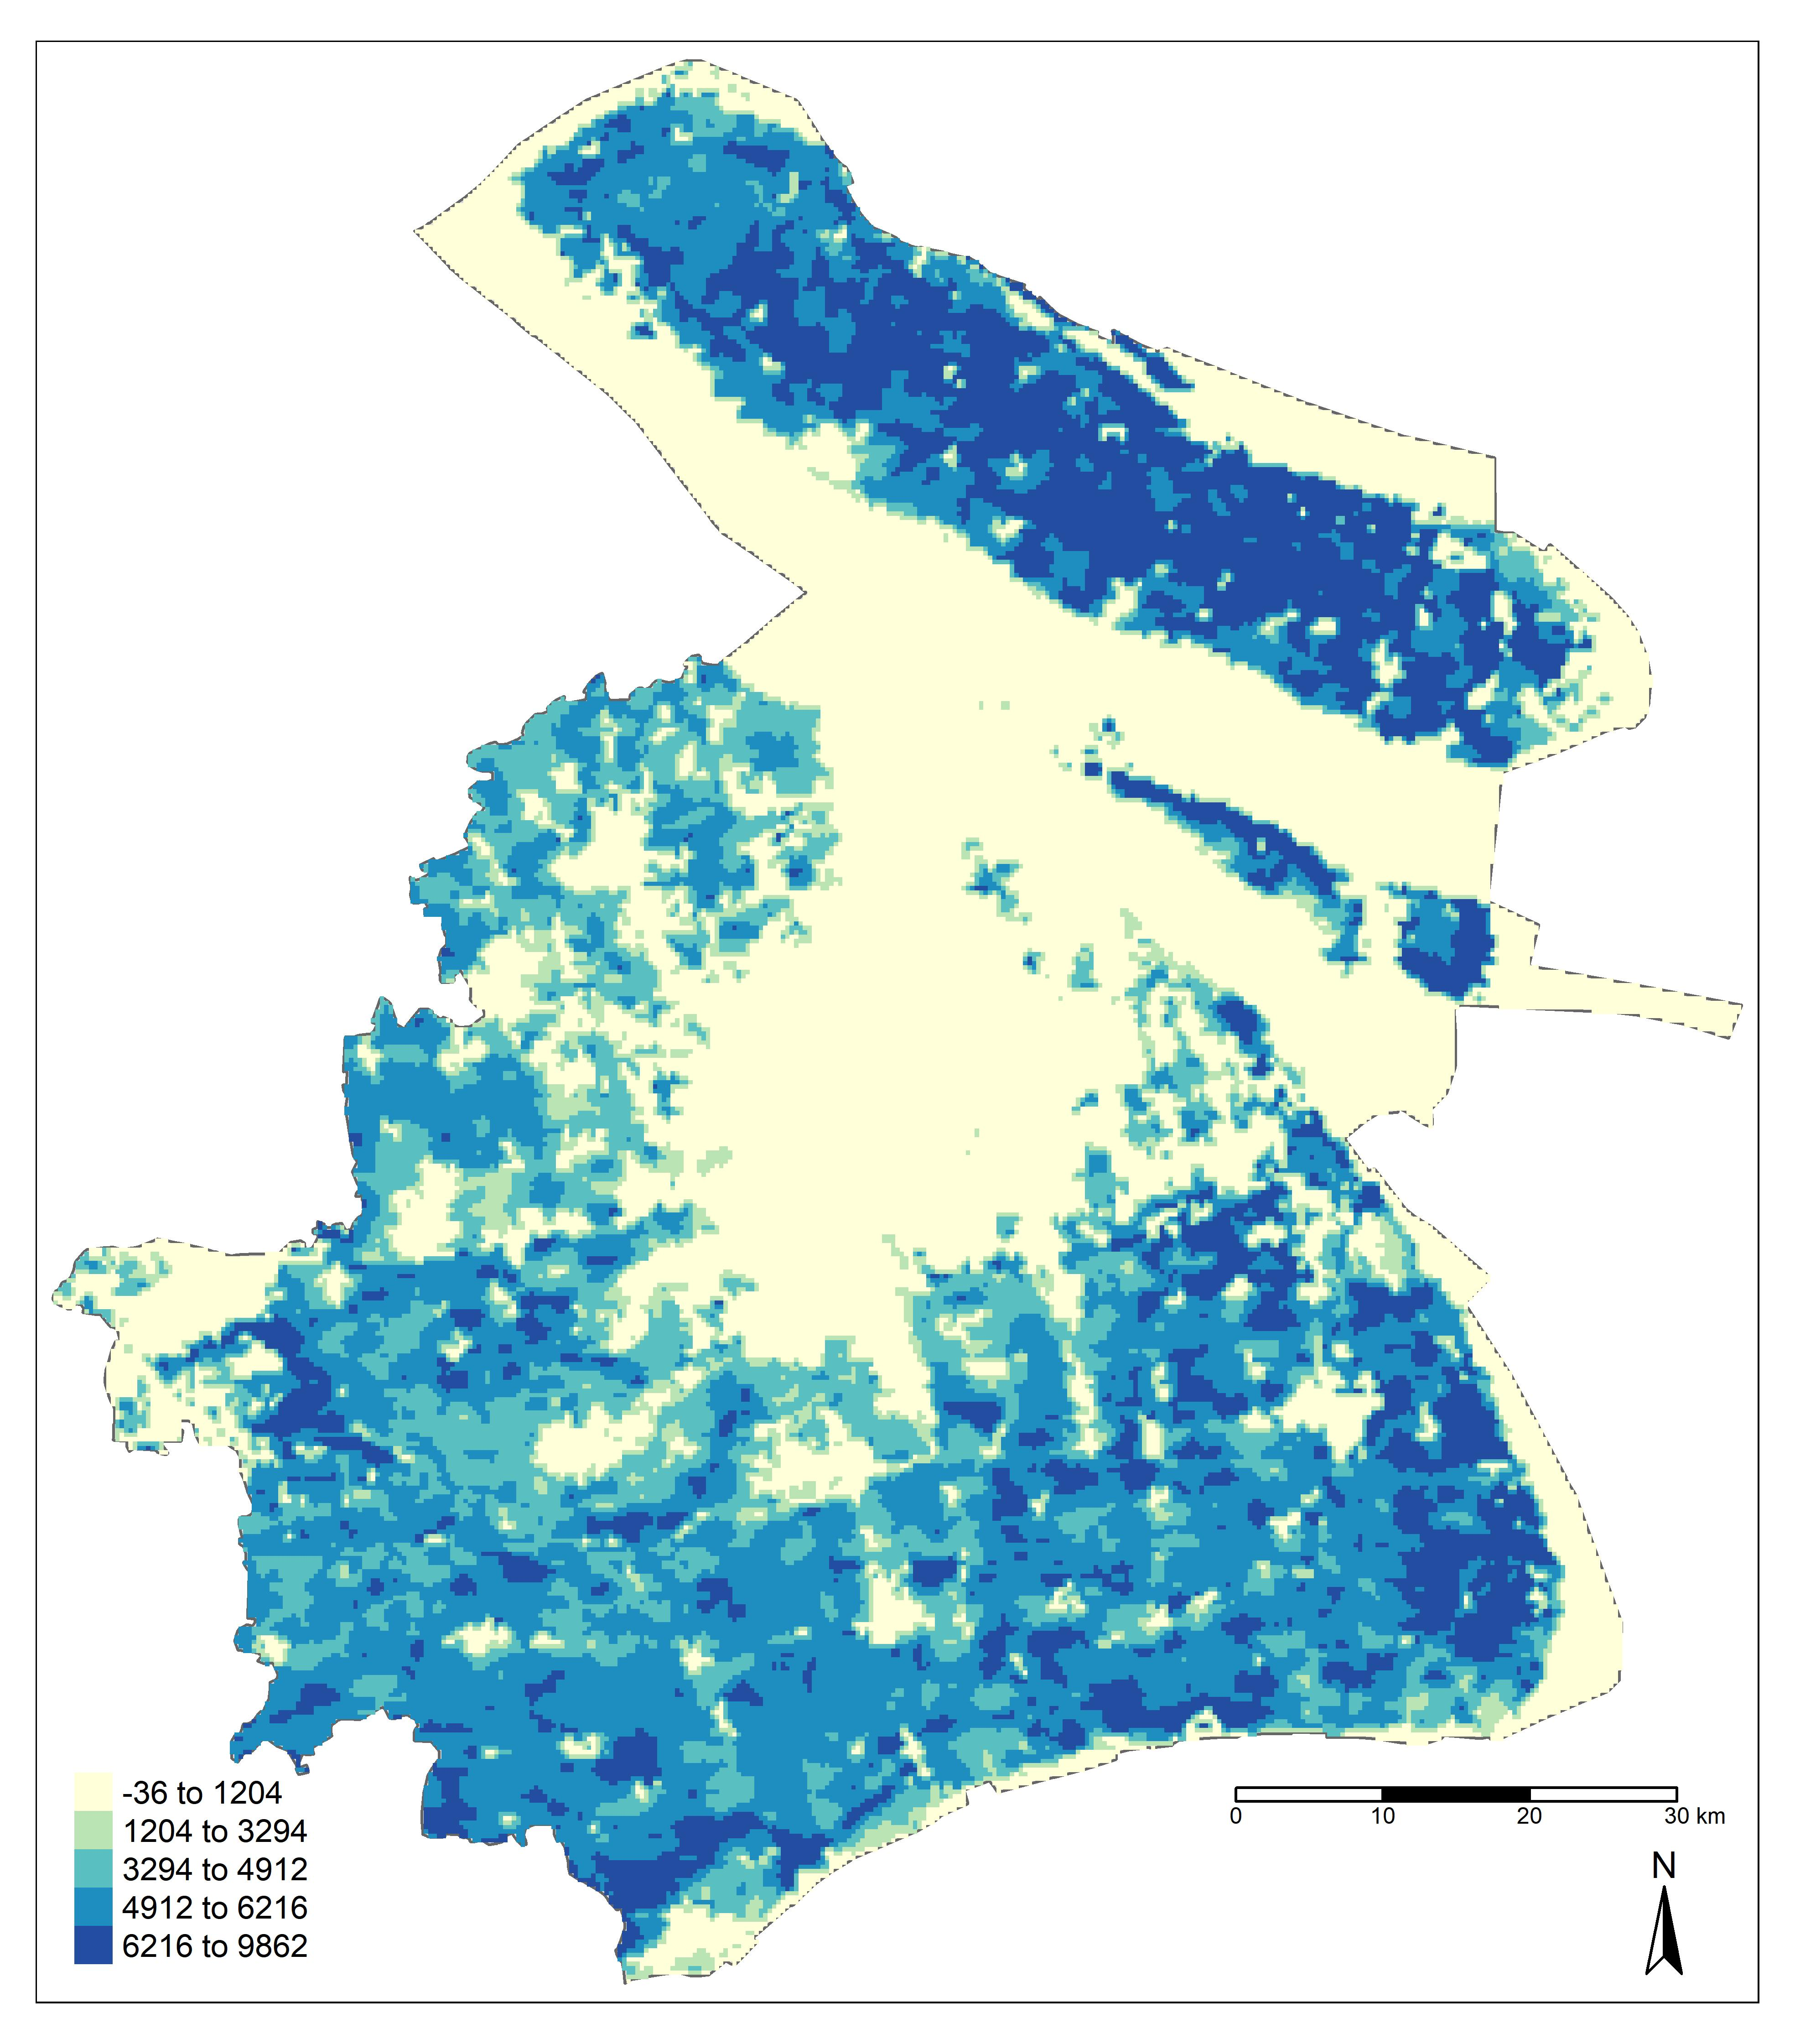
\includegraphics[width=6cm]{Figure/npp_sh.jpg}
}
\quad
\subfigure[PM2.5]{
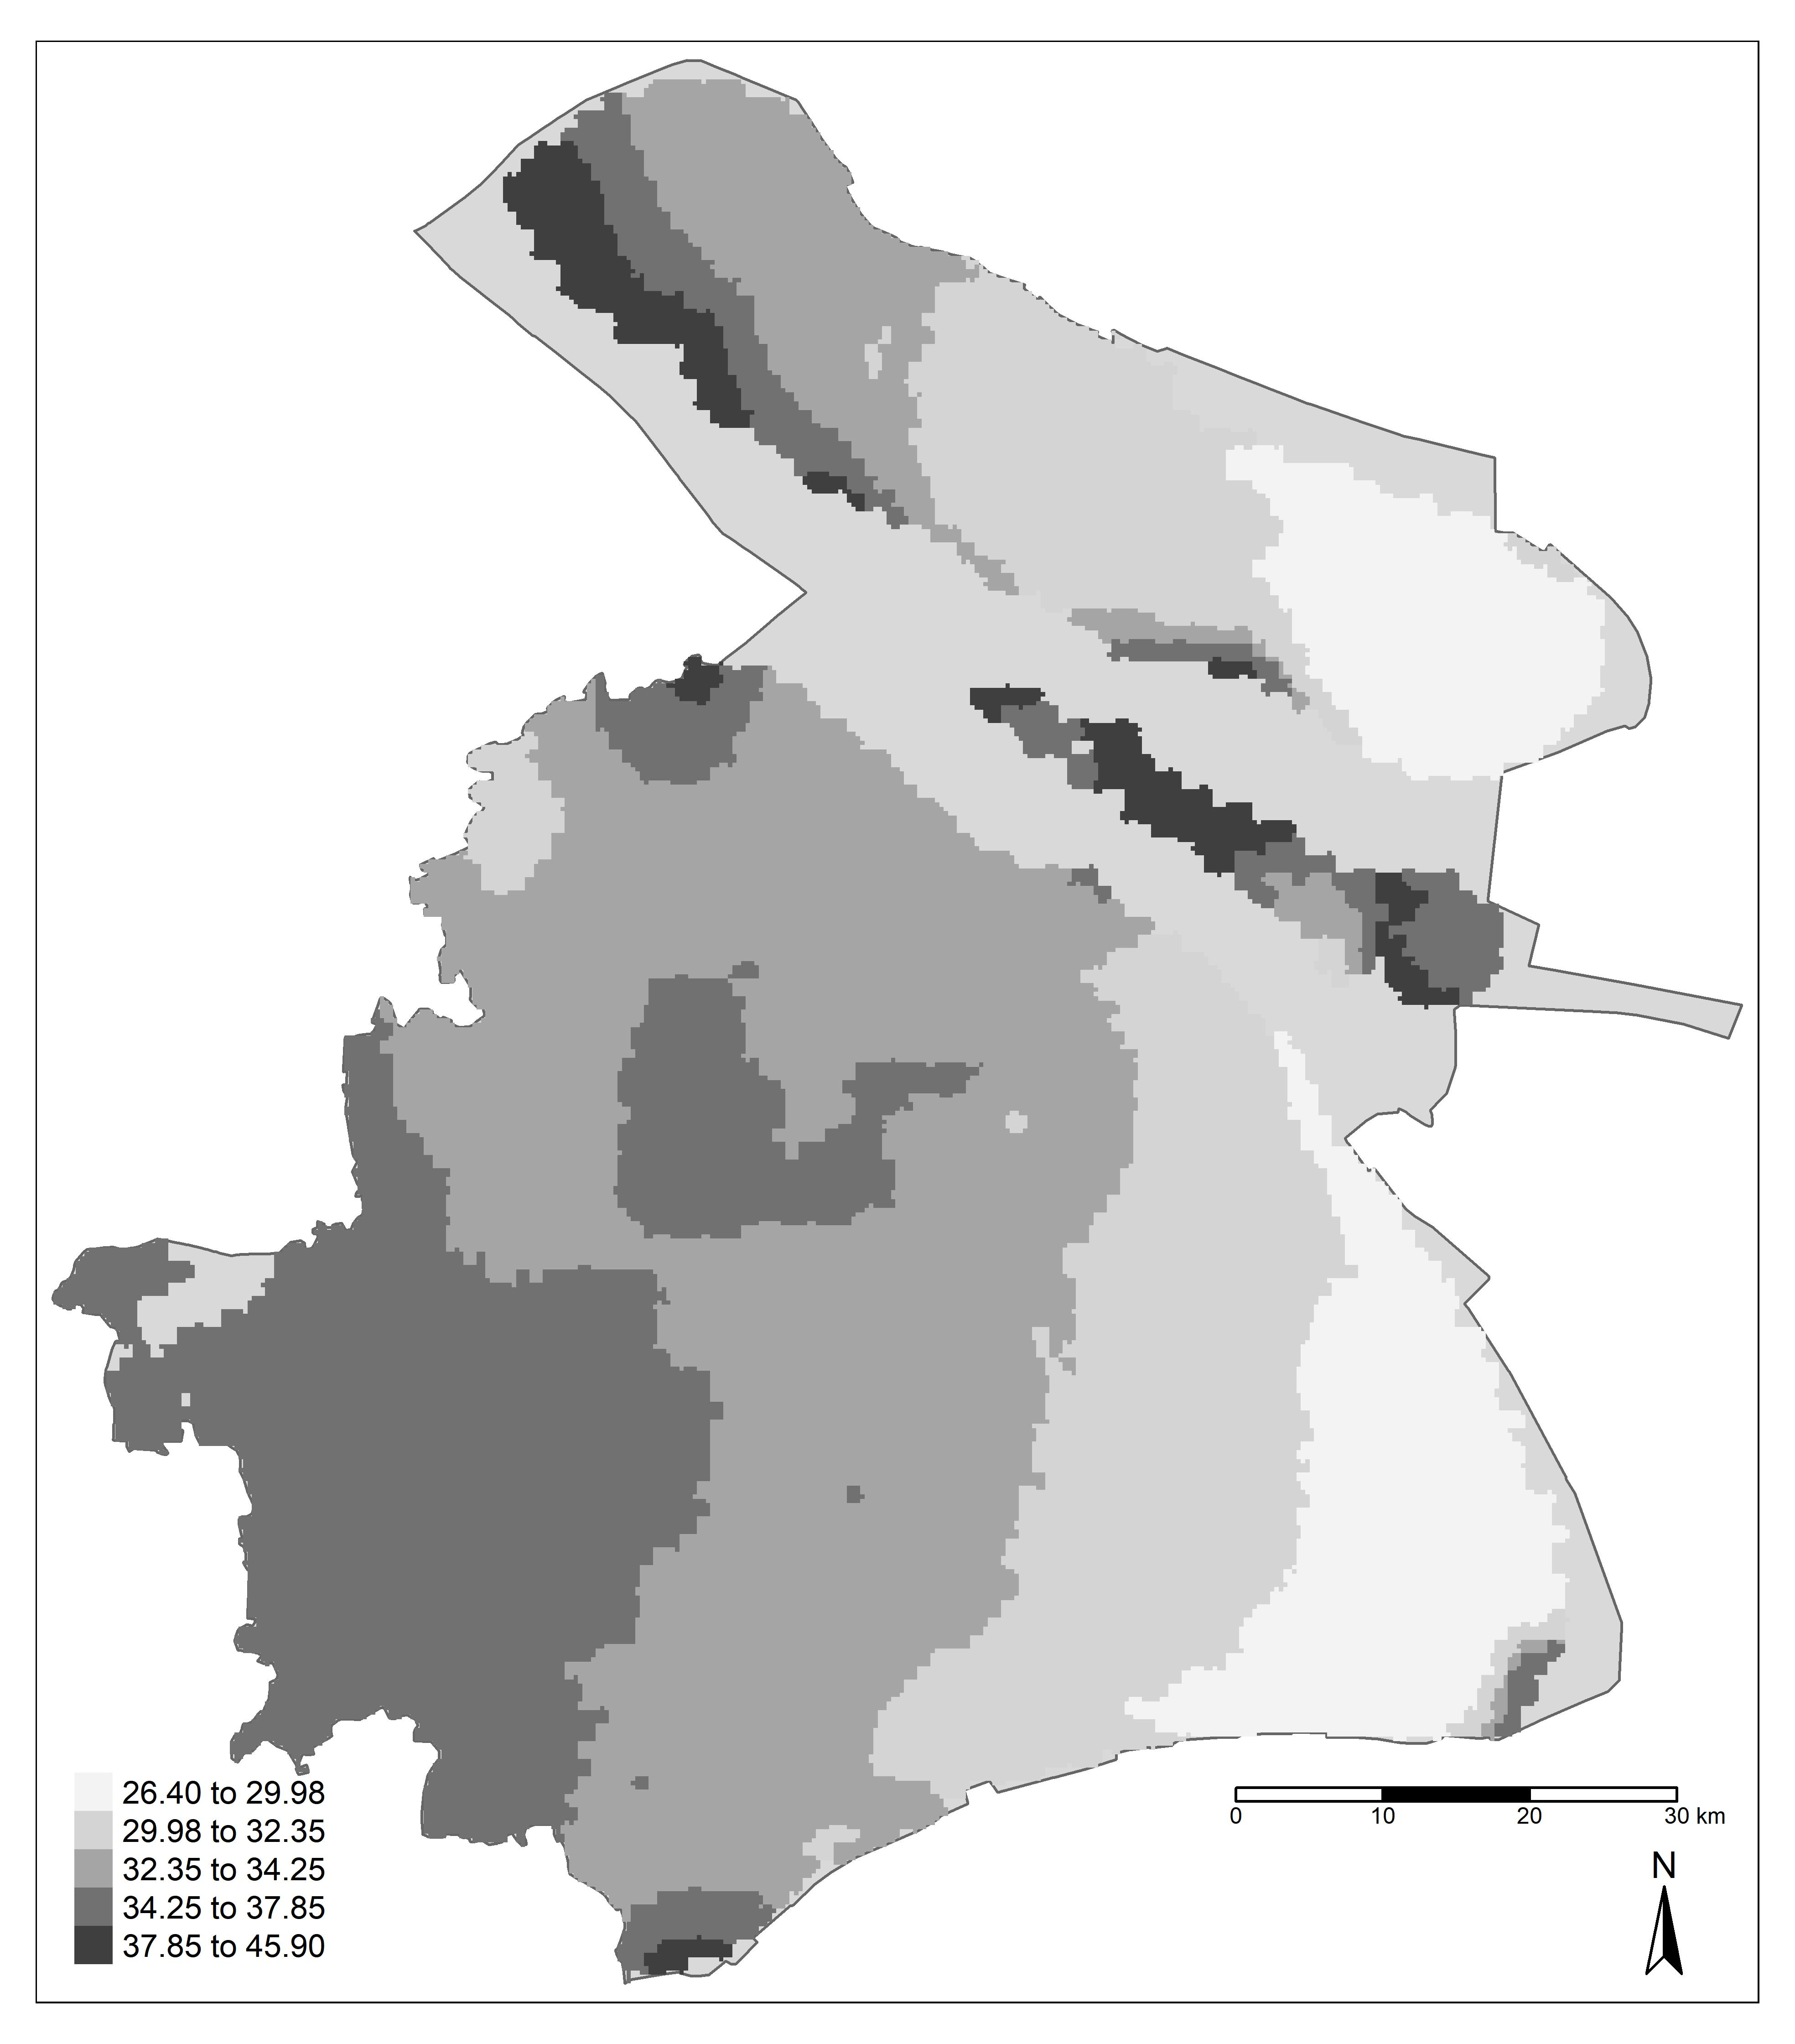
\includegraphics[width=6cm]{Figure/pm_sh.jpg}
}
\caption{Indicators of environmental system in Shanghai}
\label{esh}
\end{figure}
%%%%%%%%%%%%%%%%%%%%%%%%%%%%%%%%%%%%

\subsubsection{Environmental system indicators}
There were similarities in the spatial distribution of NPP and NDVI. The spatial layout of NDVI in Guangzhou showed a “moderately dense-sparse-dense” pattern from south to north area of the city. Shanghai city, on the other hand, showed a “dense-sparse-dense” pattern. By observing the two case cities, it can be seen that the high-value areas were concentrated around the central part of the cities. Different from NDVI, NPP was generally low or even zero in the construction land, which was due to the fact that impermeable surfaces could not perform the function of carbon fixation and oxygen emission.\\

When it comes to air quality indicator, PM25 has a significant difference from the other two environmental indicators. The high concentration areas in Guangzhou were distributed in the eastern and western parts of the city. The concentration of particulates gradually increased from the south to the central part of the city and decreased from the central part to the northern part of the city and finally dropped to the lowest value. By observation, it can be found that the PM25 concentration was the lowest in the northern woodland area, and the coastal area was also relatively low.\\

While in Shanghai, PM25 concentrations gradually show a trend from high to low from southwest to northeast. The PM25 concentration also becomes gradually lower in the area near the East China Sea.\\


\subsection{Comparation of urban fringe area in time series}
As shown in Figure \ref{totaldevelop}, the figure shows the changes of urban development index and environmental index in two cities from Guangzhou and Shanghai from 2013 to 2019 in the total area. The overall growth trend showed that both cities have been growing year by year in terms of urban development and environmental index.\\

The urban development index of Guangzhou has increased from 0.19 to 0.21 from 2013 to 2019, with a total increase of 1.11 times in these years. And the environmental index increased from 0.54 to 0.65 from 2013 to 2019, a total increase of 1.19 times.\\

%%%%%%%%%%%%%%%%%%%%%%%%%%%%%%%%%%%%
\begin{figure}[H]
\centering
\subfigure[Urban development system]{
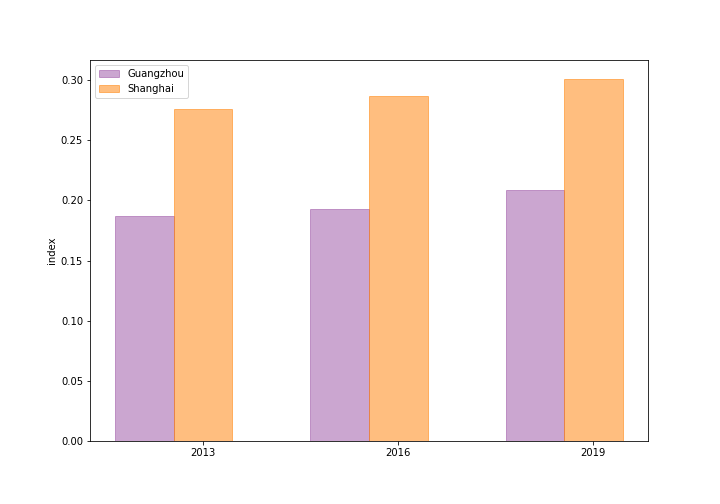
\includegraphics[width=6.5cm]{Figure/development_ur.png}
}
\quad
\subfigure[Environmental system]{
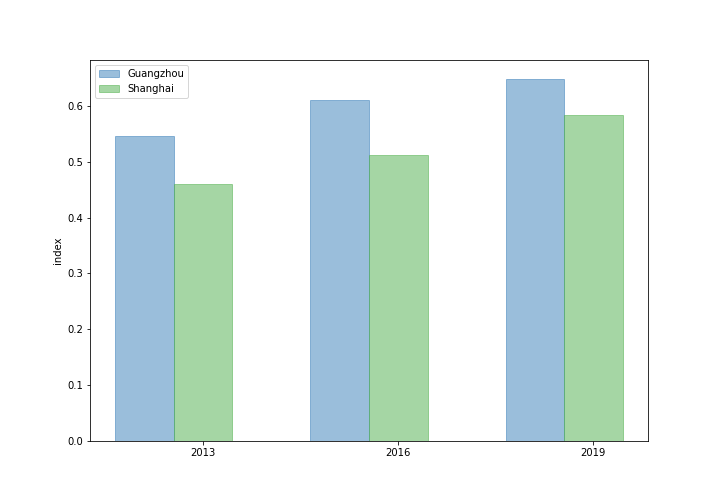
\includegraphics[width=6.5cm]{Figure/development_en.png}
}

\caption{The change of two system in total area from 2013 to 2019}
\label{totaldevelop}
\end{figure}
%%%%%%%%%%%%%%%%%%%%%%%%%%%%%%%%%%%%

On the contrary, Shanghai's urban development index increased from 0.27 to 0.30 from 2013 to 2019, a total increase of 1.09 times. And environmental index increased from 0.46 to 0.58 from 2013 to 2019, a total increase of 1.27 times.\\

It is obvious that Shanghai could have a significantly higher level of development than Guangzhou in the overall urban development index, while Guangzhou had an advantage in the environmental index compared to Shanghai. However, in terms of growth rate from 2013 to 2019, Guangzhou had a faster growth rate than Shanghai in terms of urban development, but slower than Shanghai in terms of environmental development.\\

When it comes to the change of two indicators in urban fringe area in Figure \ref{zonaldevelop}. The urban development index of Shanghai was still higher than that of Guangzhou in the urban fringe area unlike the total area, but the difference between the two cities was not significant. This would further prove that the identification of urban fringe area could effectively identify the urban fringe area. The urban development index of Guangzhou has increased from 0.33 to 0.36, with a total increase of 1.11 times. The urban development index of Shanghai increases from 0.34 to 0.36, with a total increase of 1.09 times.\\

%%%%%%%%%%%%%%%%%%%%%%%%%%%%%%%%%%%%
\begin{figure}[H]
\centering
\subfigure[Urban development system]{
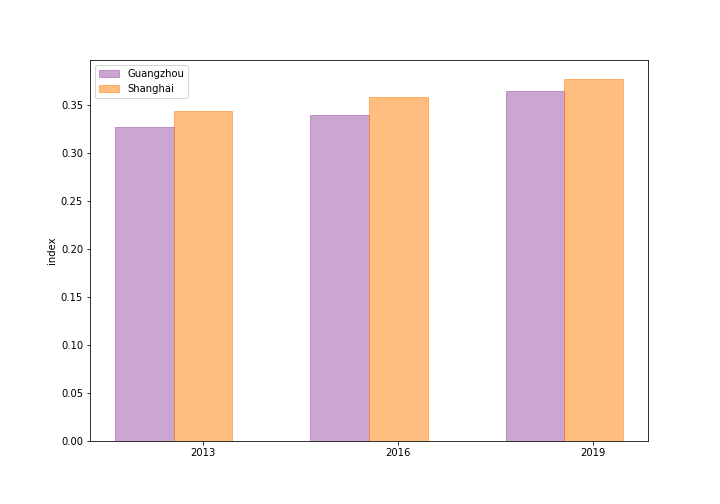
\includegraphics[width=6.5cm]{Figure/development_ur2.png}
}
\quad
\subfigure[Environmental system]{
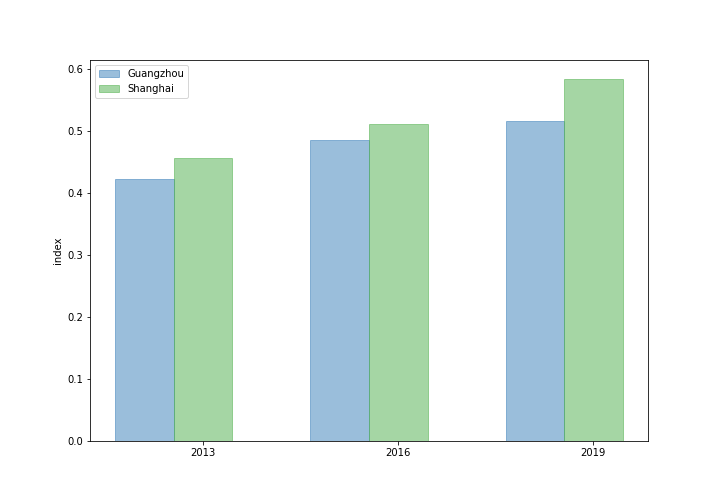
\includegraphics[width=6.5cm]{Figure/development_en2.png}
}

\caption{The change of two system in urban fringe area from 2013 to 2019}
\label{zonaldevelop}
\end{figure}
%%%%%%%%%%%%%%%%%%%%%%%%%%%%%%%%%%%%

At the same time, unlike the total area, Shanghai would have a higher environmental index than Guangzhou in the urban fringe area. The environmental index of Guangzhou increased from 0.42 to 0.51 by a total increasing ratio of 1.22. The environmental index of Shanghai increased from 0.46 to 0.58 by a total increasing ratio of 1.28. It is worth mentioning that the environmental index of Shanghai increased more from 2016 to 2019.\\

When focusing on the 3 indicators in urban development system (Figure \ref{ratiourban}), the study showed that the growth rate of the 3 indicators in both cities was always greater than 1 from 2013 to 2019. This also indicated that the level of urban construction was always in a state of development. However, the graph showed that the growth rate of AL and CL has slowed down from 2016 to 2019. This would also demonstrate that the rate of urban expansion was decreasing. In contrast to this, the growth rate of NT increased significantly from 2016 to 2019, which would also means that the overall level of urban land use was gradually increasing.\\

%%%%%%%%%%%%%%%%%%%%%%%%%%%%%%%%%%%%
\begin{figure}[H]
\centering
\subfigure[Guangzhou]{
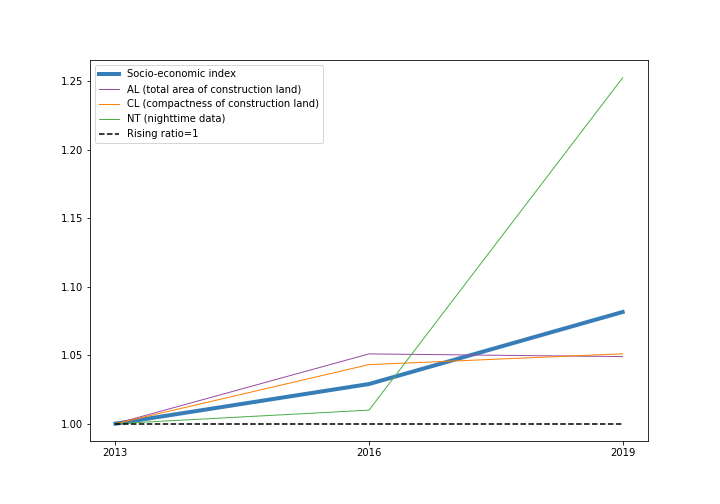
\includegraphics[width=6.5cm]{Figure/urbangz20821.png}
}
\quad
\subfigure[Shanghai]{
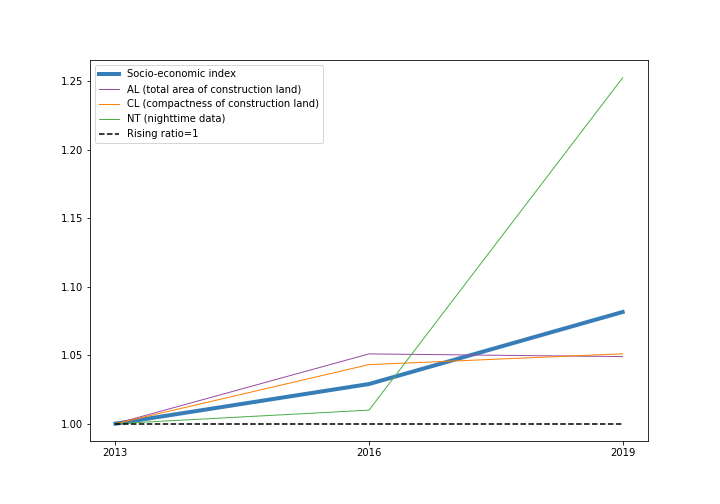
\includegraphics[width=6.5cm]{Figure/urbansh20821.png}
}

\caption{The raising ratio of urban development system from 2013 to 2019}
\label{ratiourban}
\end{figure}
%%%%%%%%%%%%%%%%%%%%%%%%%%%%%%%%%%%%

When it comes to 3 indicators in the environmental system (Figure \ref{ratioenvir}), the PM2.5 growth rate in both cities has been substantially less than 1 from 2013 to 2019, which would prove that air pollution was being gradually addressed. In Guangzhou, the NDVI value has been stable for six years, while the NPP has increased 1.13 times from 2016 to 2019. This could also prove that the level of carbon fixation and oxygen emission in Guangzhou has been improved. In contrast, the decline of NDVI and NPP in Shanghai was gradually increasing, which would be also further evidence that the ecological space was gradually being damaged while the city was developing. This is also something that needs more attention for future development.\\

%%%%%%%%%%%%%%%%%%%%%%%%%%%%%%%%%%%%
\begin{figure}[H]
\centering
\subfigure[Guangzhou]{
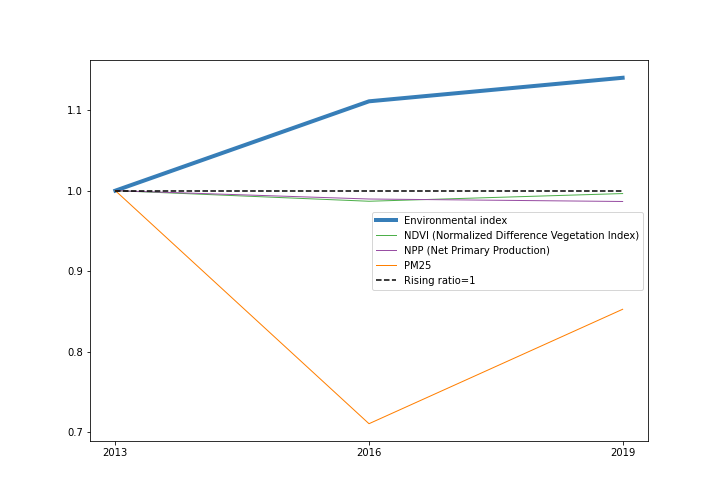
\includegraphics[width=6.5cm]{Figure/envirgz20821.png}
}
\quad
\subfigure[Shanghai]{
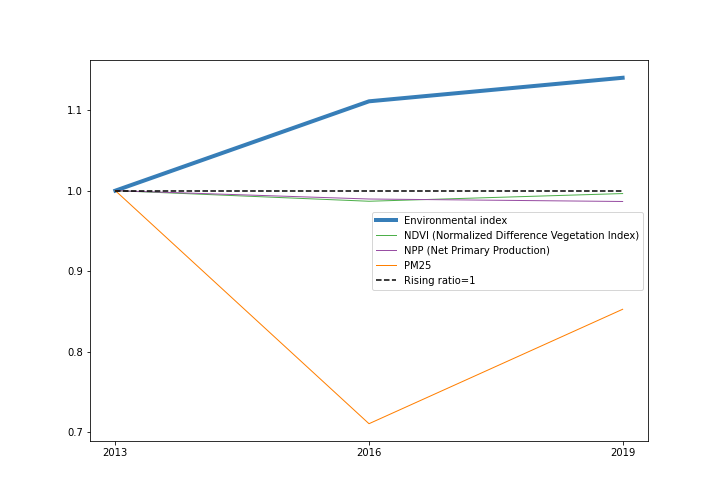
\includegraphics[width=6.5cm]{Figure/envirsh20821.png}
}

\caption{The raising ratio of environmental system from 2013 to 2019}
\label{ratioenvir}
\end{figure}
%%%%%%%%%%%%%%%%%%%%%%%%%%%%%%%%%%%%